\documentclass[10pt,twocolumn]{article}
\usepackage[margin=0.8in]{geometry}
\usepackage{graphicx}
\usepackage{booktabs}
\usepackage{amsmath}
\usepackage{amssymb}
\usepackage{hyperref}
\usepackage{natbib}
\renewcommand{\topfraction}{0.9}
\renewcommand{\dbltopfraction}{0.9}
\renewcommand{\textfraction}{0.07}
\renewcommand{\floatpagefraction}{0.7}
\renewcommand{\dblfloatpagefraction}{0.7}
% Result macros are generated with ASCII hyphens; read them with an active
% hyphen so that negative numbers print with a true minus sign.
\begingroup\lccode`\~=`\-\lowercase{\endgroup\def~}{\ensuremath{-}}
\catcode`\-=\active
% Auto-generated by autoloop/make_results_tex.py. Do not hand-edit.
% Every empirical number in paper/main.tex is accessed via \res{<key>}.

\expandafter\def\csname res@c3hc_s_each_c\endcsname{-0.173}
\expandafter\def\csname res@c3hc_s_each_c_ci\endcsname{[-0.408, +0.050]}
\expandafter\def\csname res@c3hc_s_each_dp\endcsname{+3.255}
\expandafter\def\csname res@c3hc_s_each_dp_ci\endcsname{[+2.834, +3.874]}
\expandafter\def\csname res@c3hc_s_each_f\endcsname{0.070}
\expandafter\def\csname res@c3hc_s_each_f_ci\endcsname{[NA, NA]}
\expandafter\def\csname res@c3hc_s_each_h\endcsname{0.967}
\expandafter\def\csname res@c3hc_s_each_h_ci\endcsname{[NA, NA]}
\expandafter\def\csname res@c3hc_s_each_n\endcsname{143}
\expandafter\def\csname res@c3hc_s_ei_dc\endcsname{-0.255}
\expandafter\def\csname res@c3hc_s_ei_dc_ci\endcsname{[-0.515, -0.040]}
\expandafter\def\csname res@c3hc_s_ei_ddp\endcsname{+0.294}
\expandafter\def\csname res@c3hc_s_ei_ddp_ci\endcsname{[-0.173, +0.794]}
\expandafter\def\csname res@c3hc_s_ei_df\endcsname{NA}
\expandafter\def\csname res@c3hc_s_ei_df_ci\endcsname{[NA, NA]}
\expandafter\def\csname res@c3hc_s_ei_dh\endcsname{NA}
\expandafter\def\csname res@c3hc_s_ei_dh_ci\endcsname{[NA, NA]}
\expandafter\def\csname res@c3hc_s_ei_n\endcsname{143}
\expandafter\def\csname res@c3hc_s_iso_c\endcsname{+0.082}
\expandafter\def\csname res@c3hc_s_iso_c_ci\endcsname{[-0.065, +0.262]}
\expandafter\def\csname res@c3hc_s_iso_dp\endcsname{+2.961}
\expandafter\def\csname res@c3hc_s_iso_dp_ci\endcsname{[+2.514, +3.565]}
\expandafter\def\csname res@c3hc_s_iso_f\endcsname{0.056}
\expandafter\def\csname res@c3hc_s_iso_f_ci\endcsname{[NA, NA]}
\expandafter\def\csname res@c3hc_s_iso_h\endcsname{0.922}
\expandafter\def\csname res@c3hc_s_iso_h_ci\endcsname{[NA, NA]}
\expandafter\def\csname res@c3hc_s_iso_n\endcsname{143}
\expandafter\def\csname res@c3hc_s_pe_dc\endcsname{-0.416}
\expandafter\def\csname res@c3hc_s_pe_dc_ci\endcsname{[-0.761, -0.104]}
\expandafter\def\csname res@c3hc_s_pe_ddp\endcsname{+0.190}
\expandafter\def\csname res@c3hc_s_pe_ddp_ci\endcsname{[-0.421, +0.853]}
\expandafter\def\csname res@c3hc_s_pe_df\endcsname{NA}
\expandafter\def\csname res@c3hc_s_pe_df_ci\endcsname{[NA, NA]}
\expandafter\def\csname res@c3hc_s_pe_dh\endcsname{NA}
\expandafter\def\csname res@c3hc_s_pe_dh_ci\endcsname{[NA, NA]}
\expandafter\def\csname res@c3hc_s_pe_n\endcsname{143}
\expandafter\def\csname res@c3hc_s_pi_dc\endcsname{-0.671}
\expandafter\def\csname res@c3hc_s_pi_dc_ci\endcsname{[-0.966, -0.474]}
\expandafter\def\csname res@c3hc_s_pi_ddp\endcsname{+0.483}
\expandafter\def\csname res@c3hc_s_pi_ddp_ci\endcsname{[-0.141, +1.193]}
\expandafter\def\csname res@c3hc_s_pi_df\endcsname{NA}
\expandafter\def\csname res@c3hc_s_pi_df_ci\endcsname{[NA, NA]}
\expandafter\def\csname res@c3hc_s_pi_dh\endcsname{NA}
\expandafter\def\csname res@c3hc_s_pi_dh_ci\endcsname{[NA, NA]}
\expandafter\def\csname res@c3hc_s_pi_n\endcsname{143}
\expandafter\def\csname res@c3hc_s_pick_c\endcsname{-0.589}
\expandafter\def\csname res@c3hc_s_pick_c_ci\endcsname{[-0.859, -0.385]}
\expandafter\def\csname res@c3hc_s_pick_dp\endcsname{+3.445}
\expandafter\def\csname res@c3hc_s_pick_dp_ci\endcsname{[+2.953, +4.060]}
\expandafter\def\csname res@c3hc_s_pick_f\endcsname{0.126}
\expandafter\def\csname res@c3hc_s_pick_f_ci\endcsname{[NA, NA]}
\expandafter\def\csname res@c3hc_s_pick_h\endcsname{0.993}
\expandafter\def\csname res@c3hc_s_pick_h_ci\endcsname{[NA, NA]}
\expandafter\def\csname res@c3hc_s_pick_n\endcsname{143}
\expandafter\def\csname res@c3hc_u_each_c\endcsname{-0.045}
\expandafter\def\csname res@c3hc_u_each_c_ci\endcsname{[-0.304, +0.206]}
\expandafter\def\csname res@c3hc_u_each_dp\endcsname{-0.045}
\expandafter\def\csname res@c3hc_u_each_dp_ci\endcsname{[-0.452, +0.365]}
\expandafter\def\csname res@c3hc_u_each_f\endcsname{0.527}
\expandafter\def\csname res@c3hc_u_each_f_ci\endcsname{[NA, NA]}
\expandafter\def\csname res@c3hc_u_each_h\endcsname{0.509}
\expandafter\def\csname res@c3hc_u_each_h_ci\endcsname{[NA, NA]}
\expandafter\def\csname res@c3hc_u_each_n\endcsname{55}
\expandafter\def\csname res@c3hc_u_ei_dc\endcsname{-0.353}
\expandafter\def\csname res@c3hc_u_ei_dc_ci\endcsname{[-0.608, -0.103]}
\expandafter\def\csname res@c3hc_u_ei_ddp\endcsname{-0.406}
\expandafter\def\csname res@c3hc_u_ei_ddp_ci\endcsname{[-0.954, +0.112]}
\expandafter\def\csname res@c3hc_u_ei_df\endcsname{NA}
\expandafter\def\csname res@c3hc_u_ei_df_ci\endcsname{[NA, NA]}
\expandafter\def\csname res@c3hc_u_ei_dh\endcsname{NA}
\expandafter\def\csname res@c3hc_u_ei_dh_ci\endcsname{[NA, NA]}
\expandafter\def\csname res@c3hc_u_ei_n\endcsname{55}
\expandafter\def\csname res@c3hc_u_iso_c\endcsname{+0.326}
\expandafter\def\csname res@c3hc_u_iso_c_ci\endcsname{[+0.140, +0.536]}
\expandafter\def\csname res@c3hc_u_iso_dp\endcsname{+0.357}
\expandafter\def\csname res@c3hc_u_iso_dp_ci\endcsname{[-0.130, +0.877]}
\expandafter\def\csname res@c3hc_u_iso_f\endcsname{0.304}
\expandafter\def\csname res@c3hc_u_iso_f_ci\endcsname{[NA, NA]}
\expandafter\def\csname res@c3hc_u_iso_h\endcsname{0.440}
\expandafter\def\csname res@c3hc_u_iso_h_ci\endcsname{[NA, NA]}
\expandafter\def\csname res@c3hc_u_iso_n\endcsname{56}
\expandafter\def\csname res@c3hc_u_pe_dc\endcsname{-0.159}
\expandafter\def\csname res@c3hc_u_pe_dc_ci\endcsname{[-0.416, +0.094]}
\expandafter\def\csname res@c3hc_u_pe_ddp\endcsname{-0.138}
\expandafter\def\csname res@c3hc_u_pe_ddp_ci\endcsname{[-0.669, +0.363]}
\expandafter\def\csname res@c3hc_u_pe_df\endcsname{NA}
\expandafter\def\csname res@c3hc_u_pe_df_ci\endcsname{[NA, NA]}
\expandafter\def\csname res@c3hc_u_pe_dh\endcsname{NA}
\expandafter\def\csname res@c3hc_u_pe_dh_ci\endcsname{[NA, NA]}
\expandafter\def\csname res@c3hc_u_pe_n\endcsname{55}
\expandafter\def\csname res@c3hc_u_pi_dc\endcsname{-0.526}
\expandafter\def\csname res@c3hc_u_pi_dc_ci\endcsname{[-0.756, -0.315]}
\expandafter\def\csname res@c3hc_u_pi_ddp\endcsname{-0.582}
\expandafter\def\csname res@c3hc_u_pi_ddp_ci\endcsname{[-1.095, -0.106]}
\expandafter\def\csname res@c3hc_u_pi_df\endcsname{NA}
\expandafter\def\csname res@c3hc_u_pi_df_ci\endcsname{[NA, NA]}
\expandafter\def\csname res@c3hc_u_pi_dh\endcsname{NA}
\expandafter\def\csname res@c3hc_u_pi_dh_ci\endcsname{[NA, NA]}
\expandafter\def\csname res@c3hc_u_pi_n\endcsname{56}
\expandafter\def\csname res@c3hc_u_pick_c\endcsname{-0.200}
\expandafter\def\csname res@c3hc_u_pick_c_ci\endcsname{[-0.437, +0.023]}
\expandafter\def\csname res@c3hc_u_pick_dp\endcsname{-0.225}
\expandafter\def\csname res@c3hc_u_pick_dp_ci\endcsname{[-0.716, +0.227]}
\expandafter\def\csname res@c3hc_u_pick_f\endcsname{0.625}
\expandafter\def\csname res@c3hc_u_pick_f_ci\endcsname{[NA, NA]}
\expandafter\def\csname res@c3hc_u_pick_h\endcsname{0.536}
\expandafter\def\csname res@c3hc_u_pick_h_ci\endcsname{[NA, NA]}
\expandafter\def\csname res@c3hc_u_pick_n\endcsname{56}
\expandafter\def\csname res@c3hp_s_each_c\endcsname{-0.182}
\expandafter\def\csname res@c3hp_s_each_c_ci\endcsname{[-0.424, +0.046]}
\expandafter\def\csname res@c3hp_s_each_dp\endcsname{+3.221}
\expandafter\def\csname res@c3hp_s_each_dp_ci\endcsname{[+2.787, +3.851]}
\expandafter\def\csname res@c3hp_s_each_f\endcsname{0.074}
\expandafter\def\csname res@c3hp_s_each_f_ci\endcsname{[NA, NA]}
\expandafter\def\csname res@c3hp_s_each_h\endcsname{0.967}
\expandafter\def\csname res@c3hp_s_each_h_ci\endcsname{[NA, NA]}
\expandafter\def\csname res@c3hp_s_each_n\endcsname{136}
\expandafter\def\csname res@c3hp_s_ei_dc\endcsname{-0.262}
\expandafter\def\csname res@c3hp_s_ei_dc_ci\endcsname{[-0.524, -0.045]}
\expandafter\def\csname res@c3hp_s_ei_ddp\endcsname{+0.304}
\expandafter\def\csname res@c3hp_s_ei_ddp_ci\endcsname{[-0.178, +0.825]}
\expandafter\def\csname res@c3hp_s_ei_df\endcsname{NA}
\expandafter\def\csname res@c3hp_s_ei_df_ci\endcsname{[NA, NA]}
\expandafter\def\csname res@c3hp_s_ei_dh\endcsname{NA}
\expandafter\def\csname res@c3hp_s_ei_dh_ci\endcsname{[NA, NA]}
\expandafter\def\csname res@c3hp_s_ei_n\endcsname{136}
\expandafter\def\csname res@c3hp_s_iso_c\endcsname{+0.079}
\expandafter\def\csname res@c3hp_s_iso_c_ci\endcsname{[-0.072, +0.266]}
\expandafter\def\csname res@c3hp_s_iso_dp\endcsname{+2.917}
\expandafter\def\csname res@c3hp_s_iso_dp_ci\endcsname{[+2.463, +3.519]}
\expandafter\def\csname res@c3hp_s_iso_f\endcsname{0.059}
\expandafter\def\csname res@c3hp_s_iso_f_ci\endcsname{[NA, NA]}
\expandafter\def\csname res@c3hp_s_iso_h\endcsname{0.919}
\expandafter\def\csname res@c3hp_s_iso_h_ci\endcsname{[NA, NA]}
\expandafter\def\csname res@c3hp_s_iso_n\endcsname{136}
\expandafter\def\csname res@c3hp_s_pe_dc\endcsname{-0.377}
\expandafter\def\csname res@c3hp_s_pe_dc_ci\endcsname{[-0.734, -0.057]}
\expandafter\def\csname res@c3hp_s_pe_ddp\endcsname{+0.244}
\expandafter\def\csname res@c3hp_s_pe_ddp_ci\endcsname{[-0.370, +0.897]}
\expandafter\def\csname res@c3hp_s_pe_df\endcsname{NA}
\expandafter\def\csname res@c3hp_s_pe_df_ci\endcsname{[NA, NA]}
\expandafter\def\csname res@c3hp_s_pe_dh\endcsname{NA}
\expandafter\def\csname res@c3hp_s_pe_dh_ci\endcsname{[NA, NA]}
\expandafter\def\csname res@c3hp_s_pe_n\endcsname{136}
\expandafter\def\csname res@c3hp_s_pi_dc\endcsname{-0.639}
\expandafter\def\csname res@c3hp_s_pi_dc_ci\endcsname{[-0.928, -0.445]}
\expandafter\def\csname res@c3hp_s_pi_ddp\endcsname{+0.548}
\expandafter\def\csname res@c3hp_s_pi_ddp_ci\endcsname{[-0.090, +1.277]}
\expandafter\def\csname res@c3hp_s_pi_df\endcsname{NA}
\expandafter\def\csname res@c3hp_s_pi_df_ci\endcsname{[NA, NA]}
\expandafter\def\csname res@c3hp_s_pi_dh\endcsname{NA}
\expandafter\def\csname res@c3hp_s_pi_dh_ci\endcsname{[NA, NA]}
\expandafter\def\csname res@c3hp_s_pi_n\endcsname{136}
\expandafter\def\csname res@c3hp_s_pick_c\endcsname{-0.560}
\expandafter\def\csname res@c3hp_s_pick_c_ci\endcsname{[-0.838, -0.356]}
\expandafter\def\csname res@c3hp_s_pick_dp\endcsname{+3.465}
\expandafter\def\csname res@c3hp_s_pick_dp_ci\endcsname{[+2.957, +4.111]}
\expandafter\def\csname res@c3hp_s_pick_f\endcsname{0.118}
\expandafter\def\csname res@c3hp_s_pick_f_ci\endcsname{[NA, NA]}
\expandafter\def\csname res@c3hp_s_pick_h\endcsname{0.993}
\expandafter\def\csname res@c3hp_s_pick_h_ci\endcsname{[NA, NA]}
\expandafter\def\csname res@c3hp_s_pick_n\endcsname{136}
\expandafter\def\csname res@c3hp_u_each_c\endcsname{-0.060}
\expandafter\def\csname res@c3hp_u_each_c_ci\endcsname{[-0.254, +0.134]}
\expandafter\def\csname res@c3hp_u_each_dp\endcsname{+0.345}
\expandafter\def\csname res@c3hp_u_each_dp_ci\endcsname{[-0.032, +0.753]}
\expandafter\def\csname res@c3hp_u_each_f\endcsname{0.455}
\expandafter\def\csname res@c3hp_u_each_f_ci\endcsname{[NA, NA]}
\expandafter\def\csname res@c3hp_u_each_h\endcsname{0.593}
\expandafter\def\csname res@c3hp_u_each_h_ci\endcsname{[NA, NA]}
\expandafter\def\csname res@c3hp_u_each_n\endcsname{77}
\expandafter\def\csname res@c3hp_u_ei_dc\endcsname{-0.247}
\expandafter\def\csname res@c3hp_u_ei_dc_ci\endcsname{[-0.445, -0.057]}
\expandafter\def\csname res@c3hp_u_ei_ddp\endcsname{-0.178}
\expandafter\def\csname res@c3hp_u_ei_ddp_ci\endcsname{[-0.591, +0.225]}
\expandafter\def\csname res@c3hp_u_ei_df\endcsname{NA}
\expandafter\def\csname res@c3hp_u_ei_df_ci\endcsname{[NA, NA]}
\expandafter\def\csname res@c3hp_u_ei_dh\endcsname{NA}
\expandafter\def\csname res@c3hp_u_ei_dh_ci\endcsname{[NA, NA]}
\expandafter\def\csname res@c3hp_u_ei_n\endcsname{77}
\expandafter\def\csname res@c3hp_u_iso_c\endcsname{+0.201}
\expandafter\def\csname res@c3hp_u_iso_c_ci\endcsname{[+0.045, +0.369]}
\expandafter\def\csname res@c3hp_u_iso_dp\endcsname{+0.518}
\expandafter\def\csname res@c3hp_u_iso_dp_ci\endcsname{[+0.091, +0.979]}
\expandafter\def\csname res@c3hp_u_iso_f\endcsname{0.321}
\expandafter\def\csname res@c3hp_u_iso_f_ci\endcsname{[NA, NA]}
\expandafter\def\csname res@c3hp_u_iso_h\endcsname{0.524}
\expandafter\def\csname res@c3hp_u_iso_h_ci\endcsname{[NA, NA]}
\expandafter\def\csname res@c3hp_u_iso_n\endcsname{78}
\expandafter\def\csname res@c3hp_u_pe_dc\endcsname{-0.200}
\expandafter\def\csname res@c3hp_u_pe_dc_ci\endcsname{[-0.403, +0.005]}
\expandafter\def\csname res@c3hp_u_pe_ddp\endcsname{-0.245}
\expandafter\def\csname res@c3hp_u_pe_ddp_ci\endcsname{[-0.658, +0.162]}
\expandafter\def\csname res@c3hp_u_pe_df\endcsname{NA}
\expandafter\def\csname res@c3hp_u_pe_df_ci\endcsname{[NA, NA]}
\expandafter\def\csname res@c3hp_u_pe_dh\endcsname{NA}
\expandafter\def\csname res@c3hp_u_pe_dh_ci\endcsname{[NA, NA]}
\expandafter\def\csname res@c3hp_u_pe_n\endcsname{77}
\expandafter\def\csname res@c3hp_u_pi_dc\endcsname{-0.458}
\expandafter\def\csname res@c3hp_u_pi_dc_ci\endcsname{[-0.643, -0.288]}
\expandafter\def\csname res@c3hp_u_pi_ddp\endcsname{-0.453}
\expandafter\def\csname res@c3hp_u_pi_ddp_ci\endcsname{[-0.851, -0.062]}
\expandafter\def\csname res@c3hp_u_pi_df\endcsname{NA}
\expandafter\def\csname res@c3hp_u_pi_df_ci\endcsname{[NA, NA]}
\expandafter\def\csname res@c3hp_u_pi_dh\endcsname{NA}
\expandafter\def\csname res@c3hp_u_pi_dh_ci\endcsname{[NA, NA]}
\expandafter\def\csname res@c3hp_u_pi_n\endcsname{78}
\expandafter\def\csname res@c3hp_u_pick_c\endcsname{-0.257}
\expandafter\def\csname res@c3hp_u_pick_c_ci\endcsname{[-0.454, -0.065]}
\expandafter\def\csname res@c3hp_u_pick_dp\endcsname{+0.066}
\expandafter\def\csname res@c3hp_u_pick_dp_ci\endcsname{[-0.336, +0.473]}
\expandafter\def\csname res@c3hp_u_pick_f\endcsname{0.590}
\expandafter\def\csname res@c3hp_u_pick_f_ci\endcsname{[NA, NA]}
\expandafter\def\csname res@c3hp_u_pick_h\endcsname{0.615}
\expandafter\def\csname res@c3hp_u_pick_h_ci\endcsname{[NA, NA]}
\expandafter\def\csname res@c3hp_u_pick_n\endcsname{78}
\expandafter\def\csname res@c3sc_s_each_c\endcsname{-0.132}
\expandafter\def\csname res@c3sc_s_each_c_ci\endcsname{[-0.336, +0.054]}
\expandafter\def\csname res@c3sc_s_each_dp\endcsname{+2.978}
\expandafter\def\csname res@c3sc_s_each_dp_ci\endcsname{[+2.565, +3.555]}
\expandafter\def\csname res@c3sc_s_each_f\endcsname{0.085}
\expandafter\def\csname res@c3sc_s_each_f_ci\endcsname{[NA, NA]}
\expandafter\def\csname res@c3sc_s_each_h\endcsname{0.951}
\expandafter\def\csname res@c3sc_s_each_h_ci\endcsname{[NA, NA]}
\expandafter\def\csname res@c3sc_s_each_n\endcsname{142}
\expandafter\def\csname res@c3sc_s_ei_dc\endcsname{-0.061}
\expandafter\def\csname res@c3sc_s_ei_dc_ci\endcsname{[-0.262, +0.137]}
\expandafter\def\csname res@c3sc_s_ei_ddp\endcsname{+0.122}
\expandafter\def\csname res@c3sc_s_ei_ddp_ci\endcsname{[-0.379, +0.660]}
\expandafter\def\csname res@c3sc_s_ei_df\endcsname{NA}
\expandafter\def\csname res@c3sc_s_ei_df_ci\endcsname{[NA, NA]}
\expandafter\def\csname res@c3sc_s_ei_dh\endcsname{NA}
\expandafter\def\csname res@c3sc_s_ei_dh_ci\endcsname{[NA, NA]}
\expandafter\def\csname res@c3sc_s_ei_n\endcsname{140}
\expandafter\def\csname res@c3sc_s_iso_c\endcsname{-0.106}
\expandafter\def\csname res@c3sc_s_iso_c_ci\endcsname{[-0.240, +0.042]}
\expandafter\def\csname res@c3sc_s_iso_dp\endcsname{+2.919}
\expandafter\def\csname res@c3sc_s_iso_dp_ci\endcsname{[+2.477, +3.496]}
\expandafter\def\csname res@c3sc_s_iso_f\endcsname{0.085}
\expandafter\def\csname res@c3sc_s_iso_f_ci\endcsname{[NA, NA]}
\expandafter\def\csname res@c3sc_s_iso_h\endcsname{0.944}
\expandafter\def\csname res@c3sc_s_iso_h_ci\endcsname{[NA, NA]}
\expandafter\def\csname res@c3sc_s_iso_n\endcsname{141}
\expandafter\def\csname res@c3sc_s_pe_dc\endcsname{-0.389}
\expandafter\def\csname res@c3sc_s_pe_dc_ci\endcsname{[-0.737, -0.163]}
\expandafter\def\csname res@c3sc_s_pe_ddp\endcsname{+0.196}
\expandafter\def\csname res@c3sc_s_pe_ddp_ci\endcsname{[-0.372, +0.899]}
\expandafter\def\csname res@c3sc_s_pe_df\endcsname{NA}
\expandafter\def\csname res@c3sc_s_pe_df_ci\endcsname{[NA, NA]}
\expandafter\def\csname res@c3sc_s_pe_dh\endcsname{NA}
\expandafter\def\csname res@c3sc_s_pe_dh_ci\endcsname{[NA, NA]}
\expandafter\def\csname res@c3sc_s_pe_n\endcsname{142}
\expandafter\def\csname res@c3sc_s_pi_dc\endcsname{-0.416}
\expandafter\def\csname res@c3sc_s_pi_dc_ci\endcsname{[-0.726, -0.225]}
\expandafter\def\csname res@c3sc_s_pi_ddp\endcsname{+0.248}
\expandafter\def\csname res@c3sc_s_pi_ddp_ci\endcsname{[-0.350, +1.025]}
\expandafter\def\csname res@c3sc_s_pi_df\endcsname{NA}
\expandafter\def\csname res@c3sc_s_pi_df_ci\endcsname{[NA, NA]}
\expandafter\def\csname res@c3sc_s_pi_dh\endcsname{NA}
\expandafter\def\csname res@c3sc_s_pi_dh_ci\endcsname{[NA, NA]}
\expandafter\def\csname res@c3sc_s_pi_n\endcsname{141}
\expandafter\def\csname res@c3sc_s_pick_c\endcsname{-0.521}
\expandafter\def\csname res@c3sc_s_pick_c_ci\endcsname{[-0.845, -0.335]}
\expandafter\def\csname res@c3sc_s_pick_dp\endcsname{+3.181}
\expandafter\def\csname res@c3sc_s_pick_dp_ci\endcsname{[+2.687, +3.939]}
\expandafter\def\csname res@c3sc_s_pick_f\endcsname{0.140}
\expandafter\def\csname res@c3sc_s_pick_f_ci\endcsname{[NA, NA]}
\expandafter\def\csname res@c3sc_s_pick_h\endcsname{0.986}
\expandafter\def\csname res@c3sc_s_pick_h_ci\endcsname{[NA, NA]}
\expandafter\def\csname res@c3sc_s_pick_n\endcsname{143}
\expandafter\def\csname res@c3sc_u_each_c\endcsname{-0.267}
\expandafter\def\csname res@c3sc_u_each_c_ci\endcsname{[-0.483, -0.066]}
\expandafter\def\csname res@c3sc_u_each_dp\endcsname{-0.091}
\expandafter\def\csname res@c3sc_u_each_dp_ci\endcsname{[-0.598, +0.403]}
\expandafter\def\csname res@c3sc_u_each_f\endcsname{0.625}
\expandafter\def\csname res@c3sc_u_each_f_ci\endcsname{[NA, NA]}
\expandafter\def\csname res@c3sc_u_each_h\endcsname{0.589}
\expandafter\def\csname res@c3sc_u_each_h_ci\endcsname{[NA, NA]}
\expandafter\def\csname res@c3sc_u_each_n\endcsname{56}
\expandafter\def\csname res@c3sc_u_ei_dc\endcsname{-0.364}
\expandafter\def\csname res@c3sc_u_ei_dc_ci\endcsname{[-0.595, -0.151]}
\expandafter\def\csname res@c3sc_u_ei_ddp\endcsname{+0.190}
\expandafter\def\csname res@c3sc_u_ei_ddp_ci\endcsname{[-0.246, +0.645]}
\expandafter\def\csname res@c3sc_u_ei_df\endcsname{NA}
\expandafter\def\csname res@c3sc_u_ei_df_ci\endcsname{[NA, NA]}
\expandafter\def\csname res@c3sc_u_ei_dh\endcsname{NA}
\expandafter\def\csname res@c3sc_u_ei_dh_ci\endcsname{[NA, NA]}
\expandafter\def\csname res@c3sc_u_ei_n\endcsname{56}
\expandafter\def\csname res@c3sc_u_iso_c\endcsname{+0.096}
\expandafter\def\csname res@c3sc_u_iso_c_ci\endcsname{[-0.085, +0.292]}
\expandafter\def\csname res@c3sc_u_iso_dp\endcsname{-0.281}
\expandafter\def\csname res@c3sc_u_iso_dp_ci\endcsname{[-0.790, +0.198]}
\expandafter\def\csname res@c3sc_u_iso_f\endcsname{0.518}
\expandafter\def\csname res@c3sc_u_iso_f_ci\endcsname{[NA, NA]}
\expandafter\def\csname res@c3sc_u_iso_h\endcsname{0.405}
\expandafter\def\csname res@c3sc_u_iso_h_ci\endcsname{[NA, NA]}
\expandafter\def\csname res@c3sc_u_iso_n\endcsname{56}
\expandafter\def\csname res@c3sc_u_pe_dc\endcsname{-0.070}
\expandafter\def\csname res@c3sc_u_pe_dc_ci\endcsname{[-0.264, +0.119]}
\expandafter\def\csname res@c3sc_u_pe_ddp\endcsname{-0.049}
\expandafter\def\csname res@c3sc_u_pe_ddp_ci\endcsname{[-0.424, +0.339]}
\expandafter\def\csname res@c3sc_u_pe_df\endcsname{NA}
\expandafter\def\csname res@c3sc_u_pe_df_ci\endcsname{[NA, NA]}
\expandafter\def\csname res@c3sc_u_pe_dh\endcsname{NA}
\expandafter\def\csname res@c3sc_u_pe_dh_ci\endcsname{[NA, NA]}
\expandafter\def\csname res@c3sc_u_pe_n\endcsname{56}
\expandafter\def\csname res@c3sc_u_pi_dc\endcsname{-0.433}
\expandafter\def\csname res@c3sc_u_pi_dc_ci\endcsname{[-0.689, -0.202]}
\expandafter\def\csname res@c3sc_u_pi_ddp\endcsname{+0.141}
\expandafter\def\csname res@c3sc_u_pi_ddp_ci\endcsname{[-0.284, +0.567]}
\expandafter\def\csname res@c3sc_u_pi_df\endcsname{NA}
\expandafter\def\csname res@c3sc_u_pi_df_ci\endcsname{[NA, NA]}
\expandafter\def\csname res@c3sc_u_pi_dh\endcsname{NA}
\expandafter\def\csname res@c3sc_u_pi_dh_ci\endcsname{[NA, NA]}
\expandafter\def\csname res@c3sc_u_pi_n\endcsname{56}
\expandafter\def\csname res@c3sc_u_pick_c\endcsname{-0.337}
\expandafter\def\csname res@c3sc_u_pick_c_ci\endcsname{[-0.572, -0.132]}
\expandafter\def\csname res@c3sc_u_pick_dp\endcsname{-0.140}
\expandafter\def\csname res@c3sc_u_pick_dp_ci\endcsname{[-0.637, +0.367]}
\expandafter\def\csname res@c3sc_u_pick_f\endcsname{0.661}
\expandafter\def\csname res@c3sc_u_pick_f_ci\endcsname{[NA, NA]}
\expandafter\def\csname res@c3sc_u_pick_h\endcsname{0.607}
\expandafter\def\csname res@c3sc_u_pick_h_ci\endcsname{[NA, NA]}
\expandafter\def\csname res@c3sc_u_pick_n\endcsname{56}
\expandafter\def\csname res@c3sp_s_each_c\endcsname{-0.134}
\expandafter\def\csname res@c3sp_s_each_c_ci\endcsname{[-0.334, +0.048]}
\expandafter\def\csname res@c3sp_s_each_dp\endcsname{+2.926}
\expandafter\def\csname res@c3sp_s_each_dp_ci\endcsname{[+2.489, +3.504]}
\expandafter\def\csname res@c3sp_s_each_f\endcsname{0.089}
\expandafter\def\csname res@c3sp_s_each_f_ci\endcsname{[NA, NA]}
\expandafter\def\csname res@c3sp_s_each_h\endcsname{0.948}
\expandafter\def\csname res@c3sp_s_each_h_ci\endcsname{[NA, NA]}
\expandafter\def\csname res@c3sp_s_each_n\endcsname{135}
\expandafter\def\csname res@c3sp_s_ei_dc\endcsname{-0.069}
\expandafter\def\csname res@c3sp_s_ei_dc_ci\endcsname{[-0.272, +0.135]}
\expandafter\def\csname res@c3sp_s_ei_ddp\endcsname{+0.046}
\expandafter\def\csname res@c3sp_s_ei_ddp_ci\endcsname{[-0.451, +0.591]}
\expandafter\def\csname res@c3sp_s_ei_df\endcsname{NA}
\expandafter\def\csname res@c3sp_s_ei_df_ci\endcsname{[NA, NA]}
\expandafter\def\csname res@c3sp_s_ei_dh\endcsname{NA}
\expandafter\def\csname res@c3sp_s_ei_dh_ci\endcsname{[NA, NA]}
\expandafter\def\csname res@c3sp_s_ei_n\endcsname{133}
\expandafter\def\csname res@c3sp_s_iso_c\endcsname{-0.100}
\expandafter\def\csname res@c3sp_s_iso_c_ci\endcsname{[-0.243, +0.047]}
\expandafter\def\csname res@c3sp_s_iso_dp\endcsname{+2.943}
\expandafter\def\csname res@c3sp_s_iso_dp_ci\endcsname{[+2.491, +3.544]}
\expandafter\def\csname res@c3sp_s_iso_f\endcsname{0.082}
\expandafter\def\csname res@c3sp_s_iso_f_ci\endcsname{[NA, NA]}
\expandafter\def\csname res@c3sp_s_iso_h\endcsname{0.945}
\expandafter\def\csname res@c3sp_s_iso_h_ci\endcsname{[NA, NA]}
\expandafter\def\csname res@c3sp_s_iso_n\endcsname{134}
\expandafter\def\csname res@c3sp_s_pe_dc\endcsname{-0.307}
\expandafter\def\csname res@c3sp_s_pe_dc_ci\endcsname{[-0.639, -0.093]}
\expandafter\def\csname res@c3sp_s_pe_ddp\endcsname{+0.087}
\expandafter\def\csname res@c3sp_s_pe_ddp_ci\endcsname{[-0.436, +0.771]}
\expandafter\def\csname res@c3sp_s_pe_df\endcsname{NA}
\expandafter\def\csname res@c3sp_s_pe_df_ci\endcsname{[NA, NA]}
\expandafter\def\csname res@c3sp_s_pe_dh\endcsname{NA}
\expandafter\def\csname res@c3sp_s_pe_dh_ci\endcsname{[NA, NA]}
\expandafter\def\csname res@c3sp_s_pe_n\endcsname{135}
\expandafter\def\csname res@c3sp_s_pi_dc\endcsname{-0.342}
\expandafter\def\csname res@c3sp_s_pi_dc_ci\endcsname{[-0.655, -0.142]}
\expandafter\def\csname res@c3sp_s_pi_ddp\endcsname{+0.062}
\expandafter\def\csname res@c3sp_s_pi_ddp_ci\endcsname{[-0.456, +0.802]}
\expandafter\def\csname res@c3sp_s_pi_df\endcsname{NA}
\expandafter\def\csname res@c3sp_s_pi_df_ci\endcsname{[NA, NA]}
\expandafter\def\csname res@c3sp_s_pi_dh\endcsname{NA}
\expandafter\def\csname res@c3sp_s_pi_dh_ci\endcsname{[NA, NA]}
\expandafter\def\csname res@c3sp_s_pi_n\endcsname{134}
\expandafter\def\csname res@c3sp_s_pick_c\endcsname{-0.440}
\expandafter\def\csname res@c3sp_s_pick_c_ci\endcsname{[-0.755, -0.275]}
\expandafter\def\csname res@c3sp_s_pick_dp\endcsname{+3.021}
\expandafter\def\csname res@c3sp_s_pick_dp_ci\endcsname{[+2.549, +3.856]}
\expandafter\def\csname res@c3sp_s_pick_f\endcsname{0.140}
\expandafter\def\csname res@c3sp_s_pick_f_ci\endcsname{[NA, NA]}
\expandafter\def\csname res@c3sp_s_pick_h\endcsname{0.978}
\expandafter\def\csname res@c3sp_s_pick_h_ci\endcsname{[NA, NA]}
\expandafter\def\csname res@c3sp_s_pick_n\endcsname{136}
\expandafter\def\csname res@c3sp_u_each_c\endcsname{-0.266}
\expandafter\def\csname res@c3sp_u_each_c_ci\endcsname{[-0.442, -0.108]}
\expandafter\def\csname res@c3sp_u_each_dp\endcsname{+0.341}
\expandafter\def\csname res@c3sp_u_each_dp_ci\endcsname{[-0.093, +0.810]}
\expandafter\def\csname res@c3sp_u_each_f\endcsname{0.538}
\expandafter\def\csname res@c3sp_u_each_f_ci\endcsname{[NA, NA]}
\expandafter\def\csname res@c3sp_u_each_h\endcsname{0.671}
\expandafter\def\csname res@c3sp_u_each_h_ci\endcsname{[NA, NA]}
\expandafter\def\csname res@c3sp_u_each_n\endcsname{78}
\expandafter\def\csname res@c3sp_u_ei_dc\endcsname{-0.284}
\expandafter\def\csname res@c3sp_u_ei_dc_ci\endcsname{[-0.459, -0.124]}
\expandafter\def\csname res@c3sp_u_ei_ddp\endcsname{+0.251}
\expandafter\def\csname res@c3sp_u_ei_ddp_ci\endcsname{[-0.092, +0.596]}
\expandafter\def\csname res@c3sp_u_ei_df\endcsname{NA}
\expandafter\def\csname res@c3sp_u_ei_df_ci\endcsname{[NA, NA]}
\expandafter\def\csname res@c3sp_u_ei_dh\endcsname{NA}
\expandafter\def\csname res@c3sp_u_ei_dh_ci\endcsname{[NA, NA]}
\expandafter\def\csname res@c3sp_u_ei_n\endcsname{78}
\expandafter\def\csname res@c3sp_u_iso_c\endcsname{+0.019}
\expandafter\def\csname res@c3sp_u_iso_c_ci\endcsname{[-0.122, +0.172]}
\expandafter\def\csname res@c3sp_u_iso_dp\endcsname{+0.090}
\expandafter\def\csname res@c3sp_u_iso_dp_ci\endcsname{[-0.336, +0.535]}
\expandafter\def\csname res@c3sp_u_iso_f\endcsname{0.474}
\expandafter\def\csname res@c3sp_u_iso_f_ci\endcsname{[NA, NA]}
\expandafter\def\csname res@c3sp_u_iso_h\endcsname{0.511}
\expandafter\def\csname res@c3sp_u_iso_h_ci\endcsname{[NA, NA]}
\expandafter\def\csname res@c3sp_u_iso_n\endcsname{78}
\expandafter\def\csname res@c3sp_u_pe_dc\endcsname{-0.110}
\expandafter\def\csname res@c3sp_u_pe_dc_ci\endcsname{[-0.263, +0.040]}
\expandafter\def\csname res@c3sp_u_pe_ddp\endcsname{-0.102}
\expandafter\def\csname res@c3sp_u_pe_ddp_ci\endcsname{[-0.420, +0.195]}
\expandafter\def\csname res@c3sp_u_pe_df\endcsname{NA}
\expandafter\def\csname res@c3sp_u_pe_df_ci\endcsname{[NA, NA]}
\expandafter\def\csname res@c3sp_u_pe_dh\endcsname{NA}
\expandafter\def\csname res@c3sp_u_pe_dh_ci\endcsname{[NA, NA]}
\expandafter\def\csname res@c3sp_u_pe_n\endcsname{78}
\expandafter\def\csname res@c3sp_u_pi_dc\endcsname{-0.395}
\expandafter\def\csname res@c3sp_u_pi_dc_ci\endcsname{[-0.599, -0.214]}
\expandafter\def\csname res@c3sp_u_pi_ddp\endcsname{+0.149}
\expandafter\def\csname res@c3sp_u_pi_ddp_ci\endcsname{[-0.194, +0.523]}
\expandafter\def\csname res@c3sp_u_pi_df\endcsname{NA}
\expandafter\def\csname res@c3sp_u_pi_df_ci\endcsname{[NA, NA]}
\expandafter\def\csname res@c3sp_u_pi_dh\endcsname{NA}
\expandafter\def\csname res@c3sp_u_pi_dh_ci\endcsname{[NA, NA]}
\expandafter\def\csname res@c3sp_u_pi_n\endcsname{78}
\expandafter\def\csname res@c3sp_u_pick_c\endcsname{-0.376}
\expandafter\def\csname res@c3sp_u_pick_c_ci\endcsname{[-0.558, -0.197]}
\expandafter\def\csname res@c3sp_u_pick_dp\endcsname{+0.239}
\expandafter\def\csname res@c3sp_u_pick_dp_ci\endcsname{[-0.203, +0.684]}
\expandafter\def\csname res@c3sp_u_pick_f\endcsname{0.603}
\expandafter\def\csname res@c3sp_u_pick_f_ci\endcsname{[NA, NA]}
\expandafter\def\csname res@c3sp_u_pick_h\endcsname{0.692}
\expandafter\def\csname res@c3sp_u_pick_h_ci\endcsname{[NA, NA]}
\expandafter\def\csname res@c3sp_u_pick_n\endcsname{78}
\expandafter\def\csname res@c4_calls_exp\endcsname{372}
\expandafter\def\csname res@c4_calls_ok\endcsname{372}
\expandafter\def\csname res@c4_d_any3_iso\endcsname{+0.456}
\expandafter\def\csname res@c4_d_any3_iso_ci\endcsname{[+0.338, +0.574]}
\expandafter\def\csname res@c4_d_any3_iso_p\endcsname{$<0.0002$}
\expandafter\def\csname res@c4_d_maj3_iso\endcsname{+0.279}
\expandafter\def\csname res@c4_d_maj3_iso_ci\endcsname{[+0.162, +0.397]}
\expandafter\def\csname res@c4_d_maj3_iso_p\endcsname{$<0.0002$}
\expandafter\def\csname res@c4_d_maj3_p1x\endcsname{0.000}
\expandafter\def\csname res@c4_d_maj3_p1x_ci\endcsname{[-0.118, +0.118]}
\expandafter\def\csname res@c4_d_maj3_p1x_p\endcsname{0.540}
\expandafter\def\csname res@c4_n_ta\endcsname{68}
\expandafter\def\csname res@c4_n_tp\endcsname{56}
\expandafter\def\csname res@c4_parse_pct\endcsname{100.0\%}
\expandafter\def\csname res@c4_sdt_any3_c\endcsname{-0.465}
\expandafter\def\csname res@c4_sdt_any3_c_ci\endcsname{[-0.689, -0.263]}
\expandafter\def\csname res@c4_sdt_any3_dp\endcsname{-0.502}
\expandafter\def\csname res@c4_sdt_any3_dp_ci\endcsname{[-1.026, -0.016]}
\expandafter\def\csname res@c4_sdt_any3_f\endcsname{0.768}
\expandafter\def\csname res@c4_sdt_any3_f_ci\endcsname{[0.661, 0.875]}
\expandafter\def\csname res@c4_sdt_any3_h\endcsname{0.586}
\expandafter\def\csname res@c4_sdt_any3_h_ci\endcsname{[0.470, 0.702]}
\expandafter\def\csname res@c4_sdt_any3_n\endcsname{56}
\expandafter\def\csname res@c4_sdt_iso_c\endcsname{+0.326}
\expandafter\def\csname res@c4_sdt_iso_c_ci\endcsname{[+0.140, +0.526]}
\expandafter\def\csname res@c4_sdt_iso_dp\endcsname{+0.357}
\expandafter\def\csname res@c4_sdt_iso_dp_ci\endcsname{[-0.119, +0.871]}
\expandafter\def\csname res@c4_sdt_iso_f\endcsname{0.304}
\expandafter\def\csname res@c4_sdt_iso_f_ci\endcsname{[0.196, 0.429]}
\expandafter\def\csname res@c4_sdt_iso_h\endcsname{0.440}
\expandafter\def\csname res@c4_sdt_iso_h_ci\endcsname{[0.327, 0.560]}
\expandafter\def\csname res@c4_sdt_iso_n\endcsname{56}
\expandafter\def\csname res@c4_sdt_maj3_c\endcsname{-0.178}
\expandafter\def\csname res@c4_sdt_maj3_c_ci\endcsname{[-0.409, +0.044]}
\expandafter\def\csname res@c4_sdt_maj3_dp\endcsname{-0.179}
\expandafter\def\csname res@c4_sdt_maj3_dp_ci\endcsname{[-0.672, +0.283]}
\expandafter\def\csname res@c4_sdt_maj3_f\endcsname{0.607}
\expandafter\def\csname res@c4_sdt_maj3_f_ci\endcsname{[0.482, 0.732]}
\expandafter\def\csname res@c4_sdt_maj3_h\endcsname{0.536}
\expandafter\def\csname res@c4_sdt_maj3_h_ci\endcsname{[0.411, 0.661]}
\expandafter\def\csname res@c4_sdt_maj3_n\endcsname{56}
\expandafter\def\csname res@c4_sdt_pick1x_c\endcsname{-0.200}
\expandafter\def\csname res@c4_sdt_pick1x_c_ci\endcsname{[-0.441, +0.044]}
\expandafter\def\csname res@c4_sdt_pick1x_dp\endcsname{-0.225}
\expandafter\def\csname res@c4_sdt_pick1x_dp_ci\endcsname{[-0.687, +0.230]}
\expandafter\def\csname res@c4_sdt_pick1x_f\endcsname{0.625}
\expandafter\def\csname res@c4_sdt_pick1x_f_ci\endcsname{[0.500, 0.750]}
\expandafter\def\csname res@c4_sdt_pick1x_h\endcsname{0.536}
\expandafter\def\csname res@c4_sdt_pick1x_h_ci\endcsname{[0.393, 0.661]}
\expandafter\def\csname res@c4_sdt_pick1x_n\endcsname{56}
\expandafter\def\csname res@c4_sdtd_any3_iso_dc\endcsname{-0.791}
\expandafter\def\csname res@c4_sdtd_any3_iso_dc_ci\endcsname{[-1.023, -0.598]}
\expandafter\def\csname res@c4_sdtd_any3_iso_dc_pgt\endcsname{1.000}
\expandafter\def\csname res@c4_sdtd_any3_iso_dc_plt\endcsname{$<0.0002$}
\expandafter\def\csname res@c4_sdtd_any3_iso_ddp\endcsname{-0.860}
\expandafter\def\csname res@c4_sdtd_any3_iso_ddp_ci\endcsname{[-1.436, -0.347]}
\expandafter\def\csname res@c4_sdtd_any3_iso_df\endcsname{+0.464}
\expandafter\def\csname res@c4_sdtd_any3_iso_df_ci\endcsname{[+0.339, +0.589]}
\expandafter\def\csname res@c4_sdtd_any3_iso_df_plt\endcsname{1.000}
\expandafter\def\csname res@c4_sdtd_any3_iso_dh\endcsname{+0.146}
\expandafter\def\csname res@c4_sdtd_any3_iso_dh_ci\endcsname{[+0.039, +0.259]}
\expandafter\def\csname res@c4_sdtd_any3_iso_n\endcsname{56}
\expandafter\def\csname res@c4_sdtd_maj3_iso_dc\endcsname{-0.503}
\expandafter\def\csname res@c4_sdtd_maj3_iso_dc_ci\endcsname{[-0.717, -0.311]}
\expandafter\def\csname res@c4_sdtd_maj3_iso_dc_pgt\endcsname{1.000}
\expandafter\def\csname res@c4_sdtd_maj3_iso_dc_plt\endcsname{$<0.0002$}
\expandafter\def\csname res@c4_sdtd_maj3_iso_ddp\endcsname{-0.536}
\expandafter\def\csname res@c4_sdtd_maj3_iso_ddp_ci\endcsname{[-1.090, -0.025]}
\expandafter\def\csname res@c4_sdtd_maj3_iso_df\endcsname{+0.304}
\expandafter\def\csname res@c4_sdtd_maj3_iso_df_ci\endcsname{[+0.179, +0.429]}
\expandafter\def\csname res@c4_sdtd_maj3_iso_df_plt\endcsname{1.000}
\expandafter\def\csname res@c4_sdtd_maj3_iso_dh\endcsname{+0.095}
\expandafter\def\csname res@c4_sdtd_maj3_iso_dh_ci\endcsname{[-0.027, +0.223]}
\expandafter\def\csname res@c4_sdtd_maj3_iso_n\endcsname{56}
\expandafter\def\csname res@c4_ta_any3\endcsname{0.809}
\expandafter\def\csname res@c4_ta_any3_ci\endcsname{[0.706, 0.897]}
\expandafter\def\csname res@c4_ta_iso\endcsname{0.353}
\expandafter\def\csname res@c4_ta_iso_ci\endcsname{[0.235, 0.471]}
\expandafter\def\csname res@c4_ta_maj3\endcsname{0.632}
\expandafter\def\csname res@c4_ta_maj3_ci\endcsname{[0.515, 0.750]}
\expandafter\def\csname res@c4_ta_maj3u\endcsname{0.667}
\expandafter\def\csname res@c4_ta_maj3u_ci\endcsname{[0.554, 0.775]}
\expandafter\def\csname res@c4_ta_pick1x\endcsname{0.632}
\expandafter\def\csname res@c4_ta_pick1x_ci\endcsname{[0.515, 0.735]}
\expandafter\def\csname res@c4_tok_iso\endcsname{17500.5}
\expandafter\def\csname res@c4_tok_n\endcsname{124}
\expandafter\def\csname res@c4_tok_pick\endcsname{16622.0}
\expandafter\def\csname res@c4_tok_ratio\endcsname{0.950}
\expandafter\def\csname res@c4_tok_ratio_ta\endcsname{0.928}
\expandafter\def\csname res@c5o_all_cl0_dc5\endcsname{+0.200}
\expandafter\def\csname res@c5o_all_cl0_dc5_ci\endcsname{[0.000, +0.500]}
\expandafter\def\csname res@c5o_all_cl0_dc5_p\endcsname{0.105}
\expandafter\def\csname res@c5o_all_cl0_iso2\endcsname{0.100}
\expandafter\def\csname res@c5o_all_cl0_n\endcsname{10}
\expandafter\def\csname res@c5o_all_cl0_pick2\endcsname{0.300}
\expandafter\def\csname res@c5o_all_cl1_dc5\endcsname{+0.286}
\expandafter\def\csname res@c5o_all_cl1_dc5_ci\endcsname{[+0.143, +0.464]}
\expandafter\def\csname res@c5o_all_cl1_dc5_p\endcsname{$<0.0002$}
\expandafter\def\csname res@c5o_all_cl1_iso2\endcsname{0.214}
\expandafter\def\csname res@c5o_all_cl1_n\endcsname{28}
\expandafter\def\csname res@c5o_all_cl1_pick2\endcsname{0.500}
\expandafter\def\csname res@c5o_all_dc3\endcsname{+0.342}
\expandafter\def\csname res@c5o_all_dc5\endcsname{+0.263}
\expandafter\def\csname res@c5o_all_dc5_ci\endcsname{[+0.132, +0.395]}
\expandafter\def\csname res@c5o_all_dc5_p\endcsname{$<0.0002$}
\expandafter\def\csname res@c5o_all_iso2\endcsname{0.184}
\expandafter\def\csname res@c5o_all_iso2_ci\endcsname{[0.079, 0.316]}
\expandafter\def\csname res@c5o_all_n\endcsname{38}
\expandafter\def\csname res@c5o_all_pick2\endcsname{0.447}
\expandafter\def\csname res@c5o_all_pick2_ci\endcsname{[0.289, 0.605]}
\expandafter\def\csname res@c5o_all_red\endcsname{+0.079}
\expandafter\def\csname res@c5o_all_red_ci\endcsname{[-0.132, +0.289]}
\expandafter\def\csname res@c5o_corr_cl0_dc5\endcsname{+0.222}
\expandafter\def\csname res@c5o_corr_cl0_dc5_ci\endcsname{[0.000, +0.556]}
\expandafter\def\csname res@c5o_corr_cl0_dc5_p\endcsname{0.105}
\expandafter\def\csname res@c5o_corr_cl0_iso2\endcsname{0.111}
\expandafter\def\csname res@c5o_corr_cl0_n\endcsname{9}
\expandafter\def\csname res@c5o_corr_cl0_pick2\endcsname{0.333}
\expandafter\def\csname res@c5o_corr_cl1_dc5\endcsname{+0.333}
\expandafter\def\csname res@c5o_corr_cl1_dc5_ci\endcsname{[+0.167, +0.542]}
\expandafter\def\csname res@c5o_corr_cl1_dc5_p\endcsname{$<0.0002$}
\expandafter\def\csname res@c5o_corr_cl1_iso2\endcsname{0.208}
\expandafter\def\csname res@c5o_corr_cl1_n\endcsname{24}
\expandafter\def\csname res@c5o_corr_cl1_pick2\endcsname{0.542}
\expandafter\def\csname res@c5o_corr_dc3\endcsname{+0.364}
\expandafter\def\csname res@c5o_corr_dc5\endcsname{+0.303}
\expandafter\def\csname res@c5o_corr_dc5_ci\endcsname{[+0.152, +0.455]}
\expandafter\def\csname res@c5o_corr_dc5_p\endcsname{$<0.0002$}
\expandafter\def\csname res@c5o_corr_iso2\endcsname{0.182}
\expandafter\def\csname res@c5o_corr_iso2_ci\endcsname{[0.061, 0.333]}
\expandafter\def\csname res@c5o_corr_n\endcsname{33}
\expandafter\def\csname res@c5o_corr_pick2\endcsname{0.485}
\expandafter\def\csname res@c5o_corr_pick2_ci\endcsname{[0.333, 0.636]}
\expandafter\def\csname res@c5o_corr_red\endcsname{+0.061}
\expandafter\def\csname res@c5o_corr_red_ci\endcsname{[-0.182, +0.303]}
\expandafter\def\csname res@c5o_exp\endcsname{38}
\expandafter\def\csname res@c5o_ok\endcsname{38}
\expandafter\def\csname res@c5o_parse_pct\endcsname{100.0\%}
\expandafter\def\csname res@c5w_diff\endcsname{+0.302}
\expandafter\def\csname res@c5w_diff_ci\endcsname{[+0.163, +0.442]}
\expandafter\def\csname res@c5w_diff_p\endcsname{$<0.0002$}
\expandafter\def\csname res@c5w_iso2\endcsname{0.256}
\expandafter\def\csname res@c5w_iso2_ci\endcsname{[0.140, 0.395]}
\expandafter\def\csname res@c5w_n\endcsname{43}
\expandafter\def\csname res@c5w_ok\endcsname{43}
\expandafter\def\csname res@c5w_parse_pct\endcsname{100.0\%}
\expandafter\def\csname res@c5w_pick2\endcsname{0.558}
\expandafter\def\csname res@c5w_pick2_ci\endcsname{[0.419, 0.698]}
\expandafter\def\csname res@c5w_prop_base\endcsname{0.422}
\expandafter\def\csname res@c5w_vs_prop\endcsname{+0.137}
\expandafter\def\csname res@c6_gemini_all_each_c\endcsname{-0.299}
\expandafter\def\csname res@c6_gemini_all_each_c_ci\endcsname{[-0.476, -0.137]}
\expandafter\def\csname res@c6_gemini_all_each_dp\endcsname{+1.562}
\expandafter\def\csname res@c6_gemini_all_each_dp_ci\endcsname{[+1.152, +2.043]}
\expandafter\def\csname res@c6_gemini_all_each_f\endcsname{0.313}
\expandafter\def\csname res@c6_gemini_all_each_f_ci\endcsname{[0.222, 0.404]}
\expandafter\def\csname res@c6_gemini_all_each_h\endcsname{0.864}
\expandafter\def\csname res@c6_gemini_all_each_h_ci\endcsname{[0.793, 0.924]}
\expandafter\def\csname res@c6_gemini_all_each_n\endcsname{99}
\expandafter\def\csname res@c6_gemini_all_iso_c\endcsname{-0.090}
\expandafter\def\csname res@c6_gemini_all_iso_c_ci\endcsname{[-0.204, +0.031]}
\expandafter\def\csname res@c6_gemini_all_iso_dp\endcsname{+1.376}
\expandafter\def\csname res@c6_gemini_all_iso_dp_ci\endcsname{[+0.977, +1.838]}
\expandafter\def\csname res@c6_gemini_all_iso_f\endcsname{0.273}
\expandafter\def\csname res@c6_gemini_all_iso_f_ci\endcsname{[0.182, 0.364]}
\expandafter\def\csname res@c6_gemini_all_iso_h\endcsname{0.785}
\expandafter\def\csname res@c6_gemini_all_iso_h_ci\endcsname{[0.717, 0.848]}
\expandafter\def\csname res@c6_gemini_all_iso_n\endcsname{99}
\expandafter\def\csname res@c6_gemini_all_pi_dc\endcsname{-0.280}
\expandafter\def\csname res@c6_gemini_all_pi_dc_ci\endcsname{[-0.459, -0.122]}
\expandafter\def\csname res@c6_gemini_all_pi_dc_pgt\endcsname{1.000}
\expandafter\def\csname res@c6_gemini_all_pi_dc_plt\endcsname{$<0.0002$}
\expandafter\def\csname res@c6_gemini_all_pi_ddp\endcsname{+0.154}
\expandafter\def\csname res@c6_gemini_all_pi_ddp_ci\endcsname{[-0.183, +0.513]}
\expandafter\def\csname res@c6_gemini_all_pi_df\endcsname{+0.071}
\expandafter\def\csname res@c6_gemini_all_pi_df_ci\endcsname{[0.000, +0.143]}
\expandafter\def\csname res@c6_gemini_all_pi_df_plt\endcsname{0.987}
\expandafter\def\csname res@c6_gemini_all_pi_dh\endcsname{+0.090}
\expandafter\def\csname res@c6_gemini_all_pi_dh_ci\endcsname{[+0.026, +0.156]}
\expandafter\def\csname res@c6_gemini_all_pi_n\endcsname{98}
\expandafter\def\csname res@c6_gemini_all_pick_c\endcsname{-0.364}
\expandafter\def\csname res@c6_gemini_all_pick_c_ci\endcsname{[-0.549, -0.204]}
\expandafter\def\csname res@c6_gemini_all_pick_dp\endcsname{+1.561}
\expandafter\def\csname res@c6_gemini_all_pick_dp_ci\endcsname{[+1.132, +2.085]}
\expandafter\def\csname res@c6_gemini_all_pick_f\endcsname{0.337}
\expandafter\def\csname res@c6_gemini_all_pick_f_ci\endcsname{[0.245, 0.429]}
\expandafter\def\csname res@c6_gemini_all_pick_h\endcsname{0.878}
\expandafter\def\csname res@c6_gemini_all_pick_h_ci\endcsname{[0.806, 0.939]}
\expandafter\def\csname res@c6_gemini_all_pick_n\endcsname{98}
\expandafter\def\csname res@c6_gemini_all_ta_each\endcsname{0.313}
\expandafter\def\csname res@c6_gemini_all_ta_each_ci\endcsname{[0.222, 0.404]}
\expandafter\def\csname res@c6_gemini_all_ta_iso\endcsname{0.273}
\expandafter\def\csname res@c6_gemini_all_ta_iso_ci\endcsname{[0.192, 0.364]}
\expandafter\def\csname res@c6_gemini_all_ta_pick\endcsname{0.337}
\expandafter\def\csname res@c6_gemini_all_ta_pick_ci\endcsname{[0.245, 0.429]}
\expandafter\def\csname res@c6_gemini_all_tp_each\endcsname{0.864}
\expandafter\def\csname res@c6_gemini_all_tp_iso\endcsname{0.785}
\expandafter\def\csname res@c6_gemini_all_tp_pick\endcsname{0.879}
\expandafter\def\csname res@c6_gemini_cal_r\endcsname{0.900}
\expandafter\def\csname res@c6_gemini_cal_w\endcsname{0.124}
\expandafter\def\csname res@c6_gemini_h3_err\endcsname{0.083}
\expandafter\def\csname res@c6_gemini_h3_fobs\endcsname{NA}
\expandafter\def\csname res@c6_gemini_h3_fpred\endcsname{0.730}
\expandafter\def\csname res@c6_gemini_n_all\endcsname{100}
\expandafter\def\csname res@c6_gemini_n_m\endcsname{14}
\expandafter\def\csname res@c6_gemini_n_s\endcsname{68}
\expandafter\def\csname res@c6_gemini_n_u\endcsname{18}
\expandafter\def\csname res@c6_gemini_n_u_arxiv\endcsname{16}
\expandafter\def\csname res@c6_gemini_n_u_contest\endcsname{2}
\expandafter\def\csname res@c6_gemini_parse_pct\endcsname{99.4\%}
\expandafter\def\csname res@c6_gemini_s_each_c\endcsname{-0.216}
\expandafter\def\csname res@c6_gemini_s_each_c_ci\endcsname{[-0.476, 0.000]}
\expandafter\def\csname res@c6_gemini_s_each_dp\endcsname{+2.468}
\expandafter\def\csname res@c6_gemini_s_each_dp_ci\endcsname{[+1.923, +3.238]}
\expandafter\def\csname res@c6_gemini_s_each_f\endcsname{0.149}
\expandafter\def\csname res@c6_gemini_s_each_f_ci\endcsname{[0.075, 0.239]}
\expandafter\def\csname res@c6_gemini_s_each_h\endcsname{0.933}
\expandafter\def\csname res@c6_gemini_s_each_h_ci\endcsname{[0.866, 0.985]}
\expandafter\def\csname res@c6_gemini_s_each_n\endcsname{67}
\expandafter\def\csname res@c6_gemini_s_iso_c\endcsname{-0.016}
\expandafter\def\csname res@c6_gemini_s_iso_c_ci\endcsname{[-0.189, +0.185]}
\expandafter\def\csname res@c6_gemini_s_iso_dp\endcsname{+2.067}
\expandafter\def\csname res@c6_gemini_s_iso_dp_ci\endcsname{[+1.562, +2.740]}
\expandafter\def\csname res@c6_gemini_s_iso_f\endcsname{0.149}
\expandafter\def\csname res@c6_gemini_s_iso_f_ci\endcsname{[0.075, 0.239]}
\expandafter\def\csname res@c6_gemini_s_iso_h\endcsname{0.858}
\expandafter\def\csname res@c6_gemini_s_iso_h_ci\endcsname{[0.781, 0.930]}
\expandafter\def\csname res@c6_gemini_s_iso_n\endcsname{67}
\expandafter\def\csname res@c6_gemini_s_pi_dc\endcsname{-0.481}
\expandafter\def\csname res@c6_gemini_s_pi_dc_ci\endcsname{[-0.886, -0.228]}
\expandafter\def\csname res@c6_gemini_s_pi_dc_pgt\endcsname{1.000}
\expandafter\def\csname res@c6_gemini_s_pi_dc_plt\endcsname{$<0.0002$}
\expandafter\def\csname res@c6_gemini_s_pi_ddp\endcsname{+0.518}
\expandafter\def\csname res@c6_gemini_s_pi_ddp_ci\endcsname{[0.000, +1.280]}
\expandafter\def\csname res@c6_gemini_s_pi_df\endcsname{+0.060}
\expandafter\def\csname res@c6_gemini_s_pi_df_ci\endcsname{[0.000, +0.134]}
\expandafter\def\csname res@c6_gemini_s_pi_df_plt\endcsname{0.980}
\expandafter\def\csname res@c6_gemini_s_pi_dh\endcsname{+0.112}
\expandafter\def\csname res@c6_gemini_s_pi_dh_ci\endcsname{[+0.042, +0.189]}
\expandafter\def\csname res@c6_gemini_s_pi_n\endcsname{67}
\expandafter\def\csname res@c6_gemini_s_pick_c\endcsname{-0.497}
\expandafter\def\csname res@c6_gemini_s_pick_c_ci\endcsname{[-0.847, -0.281]}
\expandafter\def\csname res@c6_gemini_s_pick_dp\endcsname{+2.585}
\expandafter\def\csname res@c6_gemini_s_pick_dp_ci\endcsname{[+1.983, +3.457]}
\expandafter\def\csname res@c6_gemini_s_pick_f\endcsname{0.209}
\expandafter\def\csname res@c6_gemini_s_pick_f_ci\endcsname{[0.119, 0.313]}
\expandafter\def\csname res@c6_gemini_s_pick_h\endcsname{0.970}
\expandafter\def\csname res@c6_gemini_s_pick_h_ci\endcsname{[0.925, 1.000]}
\expandafter\def\csname res@c6_gemini_s_pick_n\endcsname{67}
\expandafter\def\csname res@c6_gemini_s_ta_each\endcsname{0.149}
\expandafter\def\csname res@c6_gemini_s_ta_each_ci\endcsname{[0.075, 0.239]}
\expandafter\def\csname res@c6_gemini_s_ta_iso\endcsname{0.149}
\expandafter\def\csname res@c6_gemini_s_ta_iso_ci\endcsname{[0.075, 0.239]}
\expandafter\def\csname res@c6_gemini_s_ta_pick\endcsname{0.209}
\expandafter\def\csname res@c6_gemini_s_ta_pick_ci\endcsname{[0.119, 0.313]}
\expandafter\def\csname res@c6_gemini_s_tp_each\endcsname{0.933}
\expandafter\def\csname res@c6_gemini_s_tp_iso\endcsname{0.858}
\expandafter\def\csname res@c6_gemini_s_tp_pick\endcsname{0.970}
\expandafter\def\csname res@c6_gemini_u_each_c\endcsname{-0.424}
\expandafter\def\csname res@c6_gemini_u_each_c_ci\endcsname{[-0.984, 0.000]}
\expandafter\def\csname res@c6_gemini_u_each_dp\endcsname{-0.584}
\expandafter\def\csname res@c6_gemini_u_each_dp_ci\endcsname{[-1.386, 0.000]}
\expandafter\def\csname res@c6_gemini_u_each_f\endcsname{0.778}
\expandafter\def\csname res@c6_gemini_u_each_f_ci\endcsname{[0.556, 0.944]}
\expandafter\def\csname res@c6_gemini_u_each_h\endcsname{0.556}
\expandafter\def\csname res@c6_gemini_u_each_h_ci\endcsname{[0.333, 0.778]}
\expandafter\def\csname res@c6_gemini_u_each_n\endcsname{18}
\expandafter\def\csname res@c6_gemini_u_iso_c\endcsname{-0.121}
\expandafter\def\csname res@c6_gemini_u_iso_c_ci\endcsname{[-0.377, +0.149]}
\expandafter\def\csname res@c6_gemini_u_iso_dp\endcsname{-0.022}
\expandafter\def\csname res@c6_gemini_u_iso_dp_ci\endcsname{[-0.871, +0.886]}
\expandafter\def\csname res@c6_gemini_u_iso_f\endcsname{0.556}
\expandafter\def\csname res@c6_gemini_u_iso_f_ci\endcsname{[0.333, 0.778]}
\expandafter\def\csname res@c6_gemini_u_iso_h\endcsname{0.546}
\expandafter\def\csname res@c6_gemini_u_iso_h_ci\endcsname{[0.380, 0.722]}
\expandafter\def\csname res@c6_gemini_u_iso_n\endcsname{18}
\expandafter\def\csname res@c6_gemini_u_pi_dc\endcsname{-0.050}
\expandafter\def\csname res@c6_gemini_u_pi_dc_ci\endcsname{[-0.405, +0.313]}
\expandafter\def\csname res@c6_gemini_u_pi_dc_pgt\endcsname{0.633}
\expandafter\def\csname res@c6_gemini_u_pi_dc_plt\endcsname{0.375}
\expandafter\def\csname res@c6_gemini_u_pi_ddp\endcsname{-0.472}
\expandafter\def\csname res@c6_gemini_u_pi_ddp_ci\endcsname{[-1.300, +0.239]}
\expandafter\def\csname res@c6_gemini_u_pi_df\endcsname{+0.118}
\expandafter\def\csname res@c6_gemini_u_pi_df_ci\endcsname{[-0.118, +0.353]}
\expandafter\def\csname res@c6_gemini_u_pi_df_plt\endcsname{0.900}
\expandafter\def\csname res@c6_gemini_u_pi_dh\endcsname{-0.078}
\expandafter\def\csname res@c6_gemini_u_pi_dh_ci\endcsname{[-0.265, +0.098]}
\expandafter\def\csname res@c6_gemini_u_pi_n\endcsname{17}
\expandafter\def\csname res@c6_gemini_u_pick_c\endcsname{-0.143}
\expandafter\def\csname res@c6_gemini_u_pick_c_ci\endcsname{[-0.578, +0.253]}
\expandafter\def\csname res@c6_gemini_u_pick_dp\endcsname{-0.425}
\expandafter\def\csname res@c6_gemini_u_pick_dp_ci\endcsname{[-1.349, +0.425]}
\expandafter\def\csname res@c6_gemini_u_pick_f\endcsname{0.647}
\expandafter\def\csname res@c6_gemini_u_pick_f_ci\endcsname{[0.412, 0.882]}
\expandafter\def\csname res@c6_gemini_u_pick_h\endcsname{0.471}
\expandafter\def\csname res@c6_gemini_u_pick_h_ci\endcsname{[0.235, 0.706]}
\expandafter\def\csname res@c6_gemini_u_pick_n\endcsname{17}
\expandafter\def\csname res@c6_gemini_u_ta_each\endcsname{0.778}
\expandafter\def\csname res@c6_gemini_u_ta_each_ci\endcsname{[0.611, 0.944]}
\expandafter\def\csname res@c6_gemini_u_ta_iso\endcsname{0.556}
\expandafter\def\csname res@c6_gemini_u_ta_iso_ci\endcsname{[0.333, 0.778]}
\expandafter\def\csname res@c6_gemini_u_ta_pick\endcsname{0.647}
\expandafter\def\csname res@c6_gemini_u_ta_pick_ci\endcsname{[0.412, 0.882]}
\expandafter\def\csname res@c6_gemini_u_tp_each\endcsname{0.556}
\expandafter\def\csname res@c6_gemini_u_tp_iso\endcsname{0.546}
\expandafter\def\csname res@c6_gemini_u_tp_pick\endcsname{0.500}
\expandafter\def\csname res@c6_gptoss_all_each_c\endcsname{-0.445}
\expandafter\def\csname res@c6_gptoss_all_each_c_ci\endcsname{[-0.616, -0.292]}
\expandafter\def\csname res@c6_gptoss_all_each_dp\endcsname{+0.305}
\expandafter\def\csname res@c6_gptoss_all_each_dp_ci\endcsname{[-0.084, +0.701]}
\expandafter\def\csname res@c6_gptoss_all_each_f\endcsname{0.616}
\expandafter\def\csname res@c6_gptoss_all_each_f_ci\endcsname{[0.525, 0.707]}
\expandafter\def\csname res@c6_gptoss_all_each_h\endcsname{0.727}
\expandafter\def\csname res@c6_gptoss_all_each_h_ci\endcsname{[0.636, 0.813]}
\expandafter\def\csname res@c6_gptoss_all_each_n\endcsname{99}
\expandafter\def\csname res@c6_gptoss_all_iso_c\endcsname{-0.284}
\expandafter\def\csname res@c6_gptoss_all_iso_c_ci\endcsname{[-0.395, -0.179]}
\expandafter\def\csname res@c6_gptoss_all_iso_dp\endcsname{-0.568}
\expandafter\def\csname res@c6_gptoss_all_iso_dp_ci\endcsname{[-0.968, -0.178]}
\expandafter\def\csname res@c6_gptoss_all_iso_f\endcsname{0.717}
\expandafter\def\csname res@c6_gptoss_all_iso_f_ci\endcsname{[0.626, 0.808]}
\expandafter\def\csname res@c6_gptoss_all_iso_h\endcsname{0.500}
\expandafter\def\csname res@c6_gptoss_all_iso_h_ci\endcsname{[0.431, 0.571]}
\expandafter\def\csname res@c6_gptoss_all_iso_n\endcsname{99}
\expandafter\def\csname res@c6_gptoss_all_pi_dc\endcsname{-0.194}
\expandafter\def\csname res@c6_gptoss_all_pi_dc_ci\endcsname{[-0.358, -0.036]}
\expandafter\def\csname res@c6_gptoss_all_pi_dc_pgt\endcsname{0.990}
\expandafter\def\csname res@c6_gptoss_all_pi_dc_plt\endcsname{0.010}
\expandafter\def\csname res@c6_gptoss_all_pi_ddp\endcsname{+0.673}
\expandafter\def\csname res@c6_gptoss_all_pi_ddp_ci\endcsname{[+0.268, +1.113]}
\expandafter\def\csname res@c6_gptoss_all_pi_df\endcsname{-0.051}
\expandafter\def\csname res@c6_gptoss_all_pi_df_ci\endcsname{[-0.143, +0.041]}
\expandafter\def\csname res@c6_gptoss_all_pi_df_plt\endcsname{0.165}
\expandafter\def\csname res@c6_gptoss_all_pi_dh\endcsname{+0.204}
\expandafter\def\csname res@c6_gptoss_all_pi_dh_ci\endcsname{[+0.109, +0.298]}
\expandafter\def\csname res@c6_gptoss_all_pi_n\endcsname{98}
\expandafter\def\csname res@c6_gptoss_all_pick_c\endcsname{-0.474}
\expandafter\def\csname res@c6_gptoss_all_pick_c_ci\endcsname{[-0.639, -0.323]}
\expandafter\def\csname res@c6_gptoss_all_pick_dp\endcsname{+0.113}
\expandafter\def\csname res@c6_gptoss_all_pick_dp_ci\endcsname{[-0.281, +0.517]}
\expandafter\def\csname res@c6_gptoss_all_pick_f\endcsname{0.663}
\expandafter\def\csname res@c6_gptoss_all_pick_f_ci\endcsname{[0.571, 0.755]}
\expandafter\def\csname res@c6_gptoss_all_pick_h\endcsname{0.704}
\expandafter\def\csname res@c6_gptoss_all_pick_h_ci\endcsname{[0.612, 0.786]}
\expandafter\def\csname res@c6_gptoss_all_pick_n\endcsname{98}
\expandafter\def\csname res@c6_gptoss_all_ta_each\endcsname{0.616}
\expandafter\def\csname res@c6_gptoss_all_ta_each_ci\endcsname{[0.515, 0.707]}
\expandafter\def\csname res@c6_gptoss_all_ta_iso\endcsname{0.717}
\expandafter\def\csname res@c6_gptoss_all_ta_iso_ci\endcsname{[0.626, 0.808]}
\expandafter\def\csname res@c6_gptoss_all_ta_pick\endcsname{0.663}
\expandafter\def\csname res@c6_gptoss_all_ta_pick_ci\endcsname{[0.571, 0.755]}
\expandafter\def\csname res@c6_gptoss_all_tp_each\endcsname{0.727}
\expandafter\def\csname res@c6_gptoss_all_tp_iso\endcsname{0.500}
\expandafter\def\csname res@c6_gptoss_all_tp_pick\endcsname{0.697}
\expandafter\def\csname res@c6_gptoss_cal_r\endcsname{0.790}
\expandafter\def\csname res@c6_gptoss_cal_w\endcsname{0.395}
\expandafter\def\csname res@c6_gptoss_h3_err\endcsname{0.116}
\expandafter\def\csname res@c6_gptoss_h3_fobs\endcsname{NA}
\expandafter\def\csname res@c6_gptoss_h3_fpred\endcsname{0.869}
\expandafter\def\csname res@c6_gptoss_n_all\endcsname{100}
\expandafter\def\csname res@c6_gptoss_n_m\endcsname{19}
\expandafter\def\csname res@c6_gptoss_n_s\endcsname{11}
\expandafter\def\csname res@c6_gptoss_n_u\endcsname{70}
\expandafter\def\csname res@c6_gptoss_n_u_arxiv\endcsname{38}
\expandafter\def\csname res@c6_gptoss_n_u_contest\endcsname{32}
\expandafter\def\csname res@c6_gptoss_parse_pct\endcsname{99.4\%}
\expandafter\def\csname res@c6_gptoss_s_each_c\endcsname{-0.592}
\expandafter\def\csname res@c6_gptoss_s_each_c_ci\endcsname{[-0.918, 0.000]}
\expandafter\def\csname res@c6_gptoss_s_each_dp\endcsname{+2.280}
\expandafter\def\csname res@c6_gptoss_s_each_dp_ci\endcsname{[+1.627, +3.463]}
\expandafter\def\csname res@c6_gptoss_s_each_f\endcsname{0.273}
\expandafter\def\csname res@c6_gptoss_s_each_f_ci\endcsname{[0.000, 0.545]}
\expandafter\def\csname res@c6_gptoss_s_each_h\endcsname{1.000}
\expandafter\def\csname res@c6_gptoss_s_each_h_ci\endcsname{[1.000, 1.000]}
\expandafter\def\csname res@c6_gptoss_s_each_n\endcsname{11}
\expandafter\def\csname res@c6_gptoss_s_iso_c\endcsname{-0.247}
\expandafter\def\csname res@c6_gptoss_s_iso_c_ci\endcsname{[-0.375, -0.116]}
\expandafter\def\csname res@c6_gptoss_s_iso_dp\endcsname{+1.131}
\expandafter\def\csname res@c6_gptoss_s_iso_dp_ci\endcsname{[+0.112, +2.533]}
\expandafter\def\csname res@c6_gptoss_s_iso_f\endcsname{0.364}
\expandafter\def\csname res@c6_gptoss_s_iso_f_ci\endcsname{[0.091, 0.636]}
\expandafter\def\csname res@c6_gptoss_s_iso_h\endcsname{0.818}
\expandafter\def\csname res@c6_gptoss_s_iso_h_ci\endcsname{[0.682, 0.955]}
\expandafter\def\csname res@c6_gptoss_s_iso_n\endcsname{11}
\expandafter\def\csname res@c6_gptoss_s_pi_dc\endcsname{-0.345}
\expandafter\def\csname res@c6_gptoss_s_pi_dc_ci\endcsname{[-0.650, +0.116]}
\expandafter\def\csname res@c6_gptoss_s_pi_dc_pgt\endcsname{0.965}
\expandafter\def\csname res@c6_gptoss_s_pi_dc_plt\endcsname{0.036}
\expandafter\def\csname res@c6_gptoss_s_pi_ddp\endcsname{+1.149}
\expandafter\def\csname res@c6_gptoss_s_pi_ddp_ci\endcsname{[0.000, +2.332]}
\expandafter\def\csname res@c6_gptoss_s_pi_df\endcsname{-0.091}
\expandafter\def\csname res@c6_gptoss_s_pi_df_ci\endcsname{[-0.364, +0.182]}
\expandafter\def\csname res@c6_gptoss_s_pi_df_plt\endcsname{0.378}
\expandafter\def\csname res@c6_gptoss_s_pi_dh\endcsname{+0.182}
\expandafter\def\csname res@c6_gptoss_s_pi_dh_ci\endcsname{[+0.045, +0.318]}
\expandafter\def\csname res@c6_gptoss_s_pi_n\endcsname{11}
\expandafter\def\csname res@c6_gptoss_s_pick_c\endcsname{-0.592}
\expandafter\def\csname res@c6_gptoss_s_pick_c_ci\endcsname{[-0.918, 0.000]}
\expandafter\def\csname res@c6_gptoss_s_pick_dp\endcsname{+2.280}
\expandafter\def\csname res@c6_gptoss_s_pick_dp_ci\endcsname{[+1.627, +3.463]}
\expandafter\def\csname res@c6_gptoss_s_pick_f\endcsname{0.273}
\expandafter\def\csname res@c6_gptoss_s_pick_f_ci\endcsname{[0.000, 0.545]}
\expandafter\def\csname res@c6_gptoss_s_pick_h\endcsname{1.000}
\expandafter\def\csname res@c6_gptoss_s_pick_h_ci\endcsname{[1.000, 1.000]}
\expandafter\def\csname res@c6_gptoss_s_pick_n\endcsname{11}
\expandafter\def\csname res@c6_gptoss_s_ta_each\endcsname{0.273}
\expandafter\def\csname res@c6_gptoss_s_ta_each_ci\endcsname{[0.000, 0.545]}
\expandafter\def\csname res@c6_gptoss_s_ta_iso\endcsname{0.364}
\expandafter\def\csname res@c6_gptoss_s_ta_iso_ci\endcsname{[0.091, 0.636]}
\expandafter\def\csname res@c6_gptoss_s_ta_pick\endcsname{0.273}
\expandafter\def\csname res@c6_gptoss_s_ta_pick_ci\endcsname{[0.000, 0.545]}
\expandafter\def\csname res@c6_gptoss_s_tp_each\endcsname{1.000}
\expandafter\def\csname res@c6_gptoss_s_tp_iso\endcsname{0.818}
\expandafter\def\csname res@c6_gptoss_s_tp_pick\endcsname{1.000}
\expandafter\def\csname res@c6_gptoss_u_each_c\endcsname{-0.530}
\expandafter\def\csname res@c6_gptoss_u_each_c_ci\endcsname{[-0.741, -0.345]}
\expandafter\def\csname res@c6_gptoss_u_each_dp\endcsname{-0.224}
\expandafter\def\csname res@c6_gptoss_u_each_dp_ci\endcsname{[-0.703, +0.265]}
\expandafter\def\csname res@c6_gptoss_u_each_f\endcsname{0.743}
\expandafter\def\csname res@c6_gptoss_u_each_f_ci\endcsname{[0.643, 0.843]}
\expandafter\def\csname res@c6_gptoss_u_each_h\endcsname{0.664}
\expandafter\def\csname res@c6_gptoss_u_each_h_ci\endcsname{[0.557, 0.771]}
\expandafter\def\csname res@c6_gptoss_u_each_n\endcsname{70}
\expandafter\def\csname res@c6_gptoss_u_iso_c\endcsname{-0.270}
\expandafter\def\csname res@c6_gptoss_u_iso_c_ci\endcsname{[-0.423, -0.134]}
\expandafter\def\csname res@c6_gptoss_u_iso_dp\endcsname{-1.015}
\expandafter\def\csname res@c6_gptoss_u_iso_dp_ci\endcsname{[-1.506, -0.575]}
\expandafter\def\csname res@c6_gptoss_u_iso_f\endcsname{0.786}
\expandafter\def\csname res@c6_gptoss_u_iso_f_ci\endcsname{[0.686, 0.871]}
\expandafter\def\csname res@c6_gptoss_u_iso_h\endcsname{0.405}
\expandafter\def\csname res@c6_gptoss_u_iso_h_ci\endcsname{[0.326, 0.486]}
\expandafter\def\csname res@c6_gptoss_u_iso_n\endcsname{70}
\expandafter\def\csname res@c6_gptoss_u_pi_dc\endcsname{-0.267}
\expandafter\def\csname res@c6_gptoss_u_pi_dc_ci\endcsname{[-0.460, -0.080]}
\expandafter\def\csname res@c6_gptoss_u_pi_dc_pgt\endcsname{0.998}
\expandafter\def\csname res@c6_gptoss_u_pi_dc_plt\endcsname{0.002}
\expandafter\def\csname res@c6_gptoss_u_pi_ddp\endcsname{+0.719}
\expandafter\def\csname res@c6_gptoss_u_pi_ddp_ci\endcsname{[+0.221, +1.260]}
\expandafter\def\csname res@c6_gptoss_u_pi_df\endcsname{-0.029}
\expandafter\def\csname res@c6_gptoss_u_pi_df_ci\endcsname{[-0.130, +0.072]}
\expandafter\def\csname res@c6_gptoss_u_pi_df_plt\endcsname{0.341}
\expandafter\def\csname res@c6_gptoss_u_pi_dh\endcsname{+0.249}
\expandafter\def\csname res@c6_gptoss_u_pi_dh_ci\endcsname{[+0.138, +0.357]}
\expandafter\def\csname res@c6_gptoss_u_pi_n\endcsname{69}
\expandafter\def\csname res@c6_gptoss_u_pick_c\endcsname{-0.530}
\expandafter\def\csname res@c6_gptoss_u_pick_c_ci\endcsname{[-0.730, -0.347]}
\expandafter\def\csname res@c6_gptoss_u_pick_dp\endcsname{-0.289}
\expandafter\def\csname res@c6_gptoss_u_pick_dp_ci\endcsname{[-0.785, +0.192]}
\expandafter\def\csname res@c6_gptoss_u_pick_f\endcsname{0.754}
\expandafter\def\csname res@c6_gptoss_u_pick_f_ci\endcsname{[0.652, 0.855]}
\expandafter\def\csname res@c6_gptoss_u_pick_h\endcsname{0.652}
\expandafter\def\csname res@c6_gptoss_u_pick_h_ci\endcsname{[0.536, 0.754]}
\expandafter\def\csname res@c6_gptoss_u_pick_n\endcsname{69}
\expandafter\def\csname res@c6_gptoss_u_ta_each\endcsname{0.743}
\expandafter\def\csname res@c6_gptoss_u_ta_each_ci\endcsname{[0.643, 0.843]}
\expandafter\def\csname res@c6_gptoss_u_ta_iso\endcsname{0.786}
\expandafter\def\csname res@c6_gptoss_u_ta_iso_ci\endcsname{[0.686, 0.871]}
\expandafter\def\csname res@c6_gptoss_u_ta_pick\endcsname{0.754}
\expandafter\def\csname res@c6_gptoss_u_ta_pick_ci\endcsname{[0.652, 0.855]}
\expandafter\def\csname res@c6_gptoss_u_tp_each\endcsname{0.664}
\expandafter\def\csname res@c6_gptoss_u_tp_iso\endcsname{0.405}
\expandafter\def\csname res@c6_gptoss_u_tp_pick\endcsname{0.643}
\expandafter\def\csname res@c6_n_problems\endcsname{100}
\expandafter\def\csname res@c7_m1_crec\endcsname{93.6\%}
\expandafter\def\csname res@c7_m1_extra_calls\endcsname{0.10}
\expandafter\def\csname res@c7_m1_iso_c\endcsname{+0.437}
\expandafter\def\csname res@c7_m1_iso_c_ci\endcsname{[+0.214, +0.716]}
\expandafter\def\csname res@c7_m1_iso_dp\endcsname{+0.935}
\expandafter\def\csname res@c7_m1_iso_dp_ci\endcsname{[+0.313, +1.638]}
\expandafter\def\csname res@c7_m1_iso_f\endcsname{0.175}
\expandafter\def\csname res@c7_m1_iso_f_ci\endcsname{[0.075, 0.300]}
\expandafter\def\csname res@c7_m1_iso_h\endcsname{0.512}
\expandafter\def\csname res@c7_m1_iso_h_ci\endcsname{[0.362, 0.650]}
\expandafter\def\csname res@c7_m1_iso_n\endcsname{40}
\expandafter\def\csname res@c7_m1_m1_c\endcsname{+0.391}
\expandafter\def\csname res@c7_m1_m1_c_ci\endcsname{[+0.117, +0.706]}
\expandafter\def\csname res@c7_m1_m1_dp\endcsname{+1.027}
\expandafter\def\csname res@c7_m1_m1_dp_ci\endcsname{[+0.459, +1.731]}
\expandafter\def\csname res@c7_m1_m1_f\endcsname{0.175}
\expandafter\def\csname res@c7_m1_m1_f_ci\endcsname{[0.075, 0.300]}
\expandafter\def\csname res@c7_m1_m1_h\endcsname{0.550}
\expandafter\def\csname res@c7_m1_m1_h_ci\endcsname{[0.400, 0.700]}
\expandafter\def\csname res@c7_m1_m1_n\endcsname{40}
\expandafter\def\csname res@c7_m1_mi_dc\endcsname{-0.046}
\expandafter\def\csname res@c7_m1_mi_dc_ci\endcsname{[-0.108, 0.000]}
\expandafter\def\csname res@c7_m1_mi_dc_pgt\endcsname{1.000}
\expandafter\def\csname res@c7_m1_mi_dc_plt\endcsname{0.045}
\expandafter\def\csname res@c7_m1_mi_ddp\endcsname{+0.092}
\expandafter\def\csname res@c7_m1_mi_ddp_ci\endcsname{[0.000, +0.216]}
\expandafter\def\csname res@c7_m1_mi_df\endcsname{0.000}
\expandafter\def\csname res@c7_m1_mi_df_ci\endcsname{[0.000, 0.000]}
\expandafter\def\csname res@c7_m1_mi_df_plt\endcsname{1.000}
\expandafter\def\csname res@c7_m1_mi_dh\endcsname{+0.038}
\expandafter\def\csname res@c7_m1_mi_dh_ci\endcsname{[0.000, +0.087]}
\expandafter\def\csname res@c7_m1_mi_n\endcsname{40}
\expandafter\def\csname res@c7_m1_mp_dc\endcsname{+0.670}
\expandafter\def\csname res@c7_m1_mp_dc_ci\endcsname{[+0.422, +0.981]}
\expandafter\def\csname res@c7_m1_mp_dc_pgt\endcsname{$<0.0002$}
\expandafter\def\csname res@c7_m1_mp_dc_plt\endcsname{1.000}
\expandafter\def\csname res@c7_m1_mp_ddp\endcsname{+1.090}
\expandafter\def\csname res@c7_m1_mp_ddp_ci\endcsname{[+0.536, +1.794]}
\expandafter\def\csname res@c7_m1_mp_df\endcsname{-0.450}
\expandafter\def\csname res@c7_m1_mp_df_ci\endcsname{[-0.625, -0.275]}
\expandafter\def\csname res@c7_m1_mp_df_plt\endcsname{$<0.0002$}
\expandafter\def\csname res@c7_m1_mp_dh\endcsname{-0.050}
\expandafter\def\csname res@c7_m1_mp_dh_ci\endcsname{[-0.150, +0.050]}
\expandafter\def\csname res@c7_m1_mp_n\endcsname{40}
\expandafter\def\csname res@c7_m1_n\endcsname{40}
\expandafter\def\csname res@c7_m1_pick_c\endcsname{-0.279}
\expandafter\def\csname res@c7_m1_pick_c_ci\endcsname{[-0.554, 0.000]}
\expandafter\def\csname res@c7_m1_pick_dp\endcsname{-0.064}
\expandafter\def\csname res@c7_m1_pick_dp_ci\endcsname{[-0.626, +0.471]}
\expandafter\def\csname res@c7_m1_pick_f\endcsname{0.625}
\expandafter\def\csname res@c7_m1_pick_f_ci\endcsname{[0.475, 0.775]}
\expandafter\def\csname res@c7_m1_pick_h\endcsname{0.600}
\expandafter\def\csname res@c7_m1_pick_h_ci\endcsname{[0.450, 0.750]}
\expandafter\def\csname res@c7_m1_pick_n\endcsname{40}
\expandafter\def\csname res@c7_m1_tb_ok\endcsname{8}
\expandafter\def\csname res@c7_m2h_crec\endcsname{241.5\%}
\expandafter\def\csname res@c7_m2h_g4_c\endcsname{+1.449}
\expandafter\def\csname res@c7_m2h_g4_c_ci\endcsname{[+1.066, +1.899]}
\expandafter\def\csname res@c7_m2h_g4_dp\endcsname{+0.685}
\expandafter\def\csname res@c7_m2h_g4_dp_ci\endcsname{[+0.177, +1.347]}
\expandafter\def\csname res@c7_m2h_g4_f\endcsname{0.025}
\expandafter\def\csname res@c7_m2h_g4_f_ci\endcsname{[0.000, 0.075]}
\expandafter\def\csname res@c7_m2h_g4_h\endcsname{0.125}
\expandafter\def\csname res@c7_m2h_g4_h_ci\endcsname{[0.025, 0.225]}
\expandafter\def\csname res@c7_m2h_g4_n\endcsname{40}
\expandafter\def\csname res@c7_m2h_mi_dc\endcsname{+1.013}
\expandafter\def\csname res@c7_m2h_mi_dc_ci\endcsname{[+0.650, +1.540]}
\expandafter\def\csname res@c7_m2h_mi_dc_pgt\endcsname{$<0.0002$}
\expandafter\def\csname res@c7_m2h_mi_dc_plt\endcsname{1.000}
\expandafter\def\csname res@c7_m2h_mi_ddp\endcsname{-0.250}
\expandafter\def\csname res@c7_m2h_mi_ddp_ci\endcsname{[-0.969, +0.503]}
\expandafter\def\csname res@c7_m2h_mi_df\endcsname{-0.150}
\expandafter\def\csname res@c7_m2h_mi_df_ci\endcsname{[-0.275, -0.050]}
\expandafter\def\csname res@c7_m2h_mi_df_plt\endcsname{0.002}
\expandafter\def\csname res@c7_m2h_mi_dh\endcsname{-0.387}
\expandafter\def\csname res@c7_m2h_mi_dh_ci\endcsname{[-0.537, -0.237]}
\expandafter\def\csname res@c7_m2h_mi_n\endcsname{40}
\expandafter\def\csname res@c7_m2h_mp_dc\endcsname{+1.728}
\expandafter\def\csname res@c7_m2h_mp_dc_ci\endcsname{[+1.353, +2.270]}
\expandafter\def\csname res@c7_m2h_mp_dc_pgt\endcsname{$<0.0002$}
\expandafter\def\csname res@c7_m2h_mp_dc_plt\endcsname{1.000}
\expandafter\def\csname res@c7_m2h_mp_ddp\endcsname{+0.748}
\expandafter\def\csname res@c7_m2h_mp_ddp_ci\endcsname{[+0.036, +1.600]}
\expandafter\def\csname res@c7_m2h_mp_df\endcsname{-0.600}
\expandafter\def\csname res@c7_m2h_mp_df_ci\endcsname{[-0.750, -0.450]}
\expandafter\def\csname res@c7_m2h_mp_df_plt\endcsname{$<0.0002$}
\expandafter\def\csname res@c7_m2h_mp_dh\endcsname{-0.475}
\expandafter\def\csname res@c7_m2h_mp_dh_ci\endcsname{[-0.625, -0.325]}
\expandafter\def\csname res@c7_m2h_mp_n\endcsname{40}
\expandafter\def\csname res@c7_m2h_n\endcsname{40}
\expandafter\def\csname res@c7_m2h_parse_pct\endcsname{100.0\%}
\expandafter\def\csname res@c7_m2h_raw_c\endcsname{+1.449}
\expandafter\def\csname res@c7_m2h_raw_c_ci\endcsname{[+1.066, +1.899]}
\expandafter\def\csname res@c7_m2h_raw_dp\endcsname{+0.685}
\expandafter\def\csname res@c7_m2h_raw_dp_ci\endcsname{[+0.177, +1.347]}
\expandafter\def\csname res@c7_m2h_raw_f\endcsname{0.025}
\expandafter\def\csname res@c7_m2h_raw_f_ci\endcsname{[0.000, 0.075]}
\expandafter\def\csname res@c7_m2h_raw_h\endcsname{0.125}
\expandafter\def\csname res@c7_m2h_raw_h_ci\endcsname{[0.025, 0.225]}
\expandafter\def\csname res@c7_m2h_raw_n\endcsname{40}
\expandafter\def\csname res@c7_m2m_gemini_g4_c\endcsname{+0.041}
\expandafter\def\csname res@c7_m2m_gemini_g4_c_ci\endcsname{[-0.206, +0.298]}
\expandafter\def\csname res@c7_m2m_gemini_g4_dp\endcsname{+1.549}
\expandafter\def\csname res@c7_m2m_gemini_g4_dp_ci\endcsname{[+0.892, +2.335]}
\expandafter\def\csname res@c7_m2m_gemini_g4_f\endcsname{0.200}
\expandafter\def\csname res@c7_m2m_gemini_g4_f_ci\endcsname{[0.075, 0.325]}
\expandafter\def\csname res@c7_m2m_gemini_g4_h\endcsname{0.775}
\expandafter\def\csname res@c7_m2m_gemini_g4_h_ci\endcsname{[0.650, 0.900]}
\expandafter\def\csname res@c7_m2m_gemini_g4_n\endcsname{40}
\expandafter\def\csname res@c7_m2m_gemini_mp_dc\endcsname{+0.369}
\expandafter\def\csname res@c7_m2m_gemini_mp_dc_ci\endcsname{[+0.135, +0.680]}
\expandafter\def\csname res@c7_m2m_gemini_mp_dc_pgt\endcsname{0.001}
\expandafter\def\csname res@c7_m2m_gemini_mp_dc_plt\endcsname{0.999}
\expandafter\def\csname res@c7_m2m_gemini_mp_ddp\endcsname{+0.198}
\expandafter\def\csname res@c7_m2m_gemini_mp_ddp_ci\endcsname{[-0.343, +0.733]}
\expandafter\def\csname res@c7_m2m_gemini_mp_df\endcsname{-0.154}
\expandafter\def\csname res@c7_m2m_gemini_mp_df_ci\endcsname{[-0.282, -0.051]}
\expandafter\def\csname res@c7_m2m_gemini_mp_df_plt\endcsname{0.001}
\expandafter\def\csname res@c7_m2m_gemini_mp_dh\endcsname{-0.077}
\expandafter\def\csname res@c7_m2m_gemini_mp_dh_ci\endcsname{[-0.179, +0.026]}
\expandafter\def\csname res@c7_m2m_gemini_mp_n\endcsname{39}
\expandafter\def\csname res@c7_m2m_gemini_n\endcsname{40}
\expandafter\def\csname res@c7_m2m_gemini_parse_pct\endcsname{100.0\%}
\expandafter\def\csname res@c7_m2m_gptoss_g4_c\endcsname{-0.500}
\expandafter\def\csname res@c7_m2m_gptoss_g4_c_ci\endcsname{[-0.802, -0.225]}
\expandafter\def\csname res@c7_m2m_gptoss_g4_dp\endcsname{+0.631}
\expandafter\def\csname res@c7_m2m_gptoss_g4_dp_ci\endcsname{[+0.065, +1.291]}
\expandafter\def\csname res@c7_m2m_gptoss_g4_f\endcsname{0.575}
\expandafter\def\csname res@c7_m2m_gptoss_g4_f_ci\endcsname{[0.425, 0.725]}
\expandafter\def\csname res@c7_m2m_gptoss_g4_h\endcsname{0.800}
\expandafter\def\csname res@c7_m2m_gptoss_g4_h_ci\endcsname{[0.675, 0.925]}
\expandafter\def\csname res@c7_m2m_gptoss_g4_n\endcsname{40}
\expandafter\def\csname res@c7_m2m_gptoss_mp_dc\endcsname{-0.057}
\expandafter\def\csname res@c7_m2m_gptoss_mp_dc_ci\endcsname{[-0.351, +0.221]}
\expandafter\def\csname res@c7_m2m_gptoss_mp_dc_pgt\endcsname{0.659}
\expandafter\def\csname res@c7_m2m_gptoss_mp_dc_plt\endcsname{0.349}
\expandafter\def\csname res@c7_m2m_gptoss_mp_ddp\endcsname{+0.496}
\expandafter\def\csname res@c7_m2m_gptoss_mp_ddp_ci\endcsname{[-0.031, +1.067]}
\expandafter\def\csname res@c7_m2m_gptoss_mp_df\endcsname{-0.075}
\expandafter\def\csname res@c7_m2m_gptoss_mp_df_ci\endcsname{[-0.225, +0.075]}
\expandafter\def\csname res@c7_m2m_gptoss_mp_df_plt\endcsname{0.189}
\expandafter\def\csname res@c7_m2m_gptoss_mp_dh\endcsname{+0.100}
\expandafter\def\csname res@c7_m2m_gptoss_mp_dh_ci\endcsname{[-0.025, +0.225]}
\expandafter\def\csname res@c7_m2m_gptoss_mp_n\endcsname{40}
\expandafter\def\csname res@c7_m2m_gptoss_n\endcsname{40}
\expandafter\def\csname res@c7_m2m_gptoss_parse_pct\endcsname{100.0\%}
\expandafter\def\csname res@c7_m2s_gemini_g4_c\endcsname{0.000}
\expandafter\def\csname res@c7_m2s_gemini_g4_c_ci\endcsname{[0.000, 0.000]}
\expandafter\def\csname res@c7_m2s_gemini_g4_dp\endcsname{+4.282}
\expandafter\def\csname res@c7_m2s_gemini_g4_dp_ci\endcsname{[+4.282, +4.282]}
\expandafter\def\csname res@c7_m2s_gemini_g4_f\endcsname{0.000}
\expandafter\def\csname res@c7_m2s_gemini_g4_f_ci\endcsname{[0.000, 0.000]}
\expandafter\def\csname res@c7_m2s_gemini_g4_h\endcsname{1.000}
\expandafter\def\csname res@c7_m2s_gemini_g4_h_ci\endcsname{[1.000, 1.000]}
\expandafter\def\csname res@c7_m2s_gemini_g4_n\endcsname{30}
\expandafter\def\csname res@c7_m2s_gemini_mp_dc\endcsname{+0.240}
\expandafter\def\csname res@c7_m2s_gemini_mp_dc_ci\endcsname{[0.000, +0.465]}
\expandafter\def\csname res@c7_m2s_gemini_mp_dc_pgt\endcsname{0.356}
\expandafter\def\csname res@c7_m2s_gemini_mp_dc_plt\endcsname{1.000}
\expandafter\def\csname res@c7_m2s_gemini_mp_ddp\endcsname{+0.481}
\expandafter\def\csname res@c7_m2s_gemini_mp_ddp_ci\endcsname{[0.000, +0.930]}
\expandafter\def\csname res@c7_m2s_gemini_mp_df\endcsname{-0.033}
\expandafter\def\csname res@c7_m2s_gemini_mp_df_ci\endcsname{[-0.100, 0.000]}
\expandafter\def\csname res@c7_m2s_gemini_mp_df_plt\endcsname{0.356}
\expandafter\def\csname res@c7_m2s_gemini_mp_dh\endcsname{0.000}
\expandafter\def\csname res@c7_m2s_gemini_mp_dh_ci\endcsname{[0.000, 0.000]}
\expandafter\def\csname res@c7_m2s_gemini_mp_n\endcsname{30}
\expandafter\def\csname res@c7_m2s_gemini_parse_pct\endcsname{100.0\%}
\expandafter\def\csname res@c7_m2s_gemlow_g4_c\endcsname{0.000}
\expandafter\def\csname res@c7_m2s_gemlow_g4_c_ci\endcsname{[0.000, 0.000]}
\expandafter\def\csname res@c7_m2s_gemlow_g4_dp\endcsname{+4.282}
\expandafter\def\csname res@c7_m2s_gemlow_g4_dp_ci\endcsname{[+4.282, +4.282]}
\expandafter\def\csname res@c7_m2s_gemlow_g4_f\endcsname{0.000}
\expandafter\def\csname res@c7_m2s_gemlow_g4_f_ci\endcsname{[0.000, 0.000]}
\expandafter\def\csname res@c7_m2s_gemlow_g4_h\endcsname{1.000}
\expandafter\def\csname res@c7_m2s_gemlow_g4_h_ci\endcsname{[1.000, 1.000]}
\expandafter\def\csname res@c7_m2s_gemlow_g4_n\endcsname{30}
\expandafter\def\csname res@c7_m2s_gemlow_mp_dc\endcsname{+0.240}
\expandafter\def\csname res@c7_m2s_gemlow_mp_dc_ci\endcsname{[0.000, +0.465]}
\expandafter\def\csname res@c7_m2s_gemlow_mp_dc_pgt\endcsname{0.361}
\expandafter\def\csname res@c7_m2s_gemlow_mp_dc_plt\endcsname{1.000}
\expandafter\def\csname res@c7_m2s_gemlow_mp_ddp\endcsname{+0.481}
\expandafter\def\csname res@c7_m2s_gemlow_mp_ddp_ci\endcsname{[0.000, +0.930]}
\expandafter\def\csname res@c7_m2s_gemlow_mp_df\endcsname{-0.033}
\expandafter\def\csname res@c7_m2s_gemlow_mp_df_ci\endcsname{[-0.100, 0.000]}
\expandafter\def\csname res@c7_m2s_gemlow_mp_df_plt\endcsname{0.361}
\expandafter\def\csname res@c7_m2s_gemlow_mp_dh\endcsname{0.000}
\expandafter\def\csname res@c7_m2s_gemlow_mp_dh_ci\endcsname{[0.000, 0.000]}
\expandafter\def\csname res@c7_m2s_gemlow_mp_n\endcsname{30}
\expandafter\def\csname res@c7_m2s_gemlow_parse_pct\endcsname{100.0\%}
\expandafter\def\csname res@c7_m2s_gptoss_g4_c\endcsname{+0.202}
\expandafter\def\csname res@c7_m2s_gptoss_g4_c_ci\endcsname{[-0.196, +0.667]}
\expandafter\def\csname res@c7_m2s_gptoss_g4_dp\endcsname{+2.019}
\expandafter\def\csname res@c7_m2s_gptoss_g4_dp_ci\endcsname{[+1.431, +2.949]}
\expandafter\def\csname res@c7_m2s_gptoss_g4_f\endcsname{0.100}
\expandafter\def\csname res@c7_m2s_gptoss_g4_f_ci\endcsname{[0.000, 0.200]}
\expandafter\def\csname res@c7_m2s_gptoss_g4_h\endcsname{0.800}
\expandafter\def\csname res@c7_m2s_gptoss_g4_h_ci\endcsname{[0.633, 0.933]}
\expandafter\def\csname res@c7_m2s_gptoss_g4_n\endcsname{30}
\expandafter\def\csname res@c7_m2s_gptoss_mp_dc\endcsname{+0.504}
\expandafter\def\csname res@c7_m2s_gptoss_mp_dc_ci\endcsname{[+0.083, +1.045]}
\expandafter\def\csname res@c7_m2s_gptoss_mp_dc_pgt\endcsname{0.011}
\expandafter\def\csname res@c7_m2s_gptoss_mp_dc_plt\endcsname{0.991}
\expandafter\def\csname res@c7_m2s_gptoss_mp_ddp\endcsname{-0.191}
\expandafter\def\csname res@c7_m2s_gptoss_mp_ddp_ci\endcsname{[-1.191, +0.745]}
\expandafter\def\csname res@c7_m2s_gptoss_mp_df\endcsname{-0.103}
\expandafter\def\csname res@c7_m2s_gptoss_mp_df_ci\endcsname{[-0.276, +0.069]}
\expandafter\def\csname res@c7_m2s_gptoss_mp_df_plt\endcsname{0.160}
\expandafter\def\csname res@c7_m2s_gptoss_mp_dh\endcsname{-0.138}
\expandafter\def\csname res@c7_m2s_gptoss_mp_dh_ci\endcsname{[-0.276, -0.034]}
\expandafter\def\csname res@c7_m2s_gptoss_mp_n\endcsname{29}
\expandafter\def\csname res@c7_m2s_gptoss_parse_pct\endcsname{100.0\%}
\expandafter\def\csname res@c7_m2s_haiku_g4_c\endcsname{+1.152}
\expandafter\def\csname res@c7_m2s_haiku_g4_c_ci\endcsname{[+0.948, +1.371]}
\expandafter\def\csname res@c7_m2s_haiku_g4_dp\endcsname{+1.979}
\expandafter\def\csname res@c7_m2s_haiku_g4_dp_ci\endcsname{[+1.541, +2.386]}
\expandafter\def\csname res@c7_m2s_haiku_g4_f\endcsname{0.000}
\expandafter\def\csname res@c7_m2s_haiku_g4_f_ci\endcsname{[0.000, 0.000]}
\expandafter\def\csname res@c7_m2s_haiku_g4_h\endcsname{0.433}
\expandafter\def\csname res@c7_m2s_haiku_g4_h_ci\endcsname{[0.267, 0.600]}
\expandafter\def\csname res@c7_m2s_haiku_g4_n\endcsname{30}
\expandafter\def\csname res@c7_m2s_haiku_mp_dc\endcsname{+1.380}
\expandafter\def\csname res@c7_m2s_haiku_mp_dc_ci\endcsname{[+1.071, +1.766]}
\expandafter\def\csname res@c7_m2s_haiku_mp_dc_pgt\endcsname{$<0.0002$}
\expandafter\def\csname res@c7_m2s_haiku_mp_dc_plt\endcsname{1.000}
\expandafter\def\csname res@c7_m2s_haiku_mp_ddp\endcsname{+0.321}
\expandafter\def\csname res@c7_m2s_haiku_mp_ddp_ci\endcsname{[-0.646, +1.084]}
\expandafter\def\csname res@c7_m2s_haiku_mp_df\endcsname{-0.267}
\expandafter\def\csname res@c7_m2s_haiku_mp_df_ci\endcsname{[-0.433, -0.133]}
\expandafter\def\csname res@c7_m2s_haiku_mp_df_plt\endcsname{$<0.0002$}
\expandafter\def\csname res@c7_m2s_haiku_mp_dh\endcsname{-0.433}
\expandafter\def\csname res@c7_m2s_haiku_mp_dh_ci\endcsname{[-0.600, -0.267]}
\expandafter\def\csname res@c7_m2s_haiku_mp_n\endcsname{30}
\expandafter\def\csname res@c7_m2s_haiku_parse_pct\endcsname{100.0\%}
\expandafter\def\csname res@c7_m2s_hydro_g4_c\endcsname{+0.608}
\expandafter\def\csname res@c7_m2s_hydro_g4_c_ci\endcsname{[+0.240, +0.818]}
\expandafter\def\csname res@c7_m2s_hydro_g4_dp\endcsname{+3.066}
\expandafter\def\csname res@c7_m2s_hydro_g4_dp_ci\endcsname{[+2.647, +3.802]}
\expandafter\def\csname res@c7_m2s_hydro_g4_f\endcsname{0.000}
\expandafter\def\csname res@c7_m2s_hydro_g4_f_ci\endcsname{[0.000, 0.000]}
\expandafter\def\csname res@c7_m2s_hydro_g4_h\endcsname{0.833}
\expandafter\def\csname res@c7_m2s_hydro_g4_h_ci\endcsname{[0.700, 0.967]}
\expandafter\def\csname res@c7_m2s_hydro_g4_n\endcsname{30}
\expandafter\def\csname res@c7_m2s_hydro_mp_dc\endcsname{+0.608}
\expandafter\def\csname res@c7_m2s_hydro_mp_dc_ci\endcsname{[+0.240, +0.818]}
\expandafter\def\csname res@c7_m2s_hydro_mp_dc_pgt\endcsname{0.005}
\expandafter\def\csname res@c7_m2s_hydro_mp_dc_plt\endcsname{1.000}
\expandafter\def\csname res@c7_m2s_hydro_mp_ddp\endcsname{-1.216}
\expandafter\def\csname res@c7_m2s_hydro_mp_ddp_ci\endcsname{[-1.635, -0.481]}
\expandafter\def\csname res@c7_m2s_hydro_mp_df\endcsname{0.000}
\expandafter\def\csname res@c7_m2s_hydro_mp_df_ci\endcsname{[0.000, 0.000]}
\expandafter\def\csname res@c7_m2s_hydro_mp_df_plt\endcsname{1.000}
\expandafter\def\csname res@c7_m2s_hydro_mp_dh\endcsname{-0.167}
\expandafter\def\csname res@c7_m2s_hydro_mp_dh_ci\endcsname{[-0.300, -0.033]}
\expandafter\def\csname res@c7_m2s_hydro_mp_n\endcsname{30}
\expandafter\def\csname res@c7_m2s_hydro_parse_pct\endcsname{100.0\%}
\expandafter\def\csname res@c7_m3_c\endcsname{-0.092}
\expandafter\def\csname res@c7_m3_c_ci\endcsname{[-0.376, +0.185]}
\expandafter\def\csname res@c7_m3_dp\endcsname{+0.061}
\expandafter\def\csname res@c7_m3_dp_ci\endcsname{[-0.449, +0.611]}
\expandafter\def\csname res@c7_m3_f\endcsname{0.525}
\expandafter\def\csname res@c7_m3_f_ci\endcsname{[0.375, 0.675]}
\expandafter\def\csname res@c7_m3_foil_all\endcsname{0.000}
\expandafter\def\csname res@c7_m3_h\endcsname{0.550}
\expandafter\def\csname res@c7_m3_h_ci\endcsname{[0.400, 0.700]}
\expandafter\def\csname res@c7_m3_mi_dc\endcsname{-0.529}
\expandafter\def\csname res@c7_m3_mi_dc_ci\endcsname{[-0.780, -0.314]}
\expandafter\def\csname res@c7_m3_mi_dc_pgt\endcsname{1.000}
\expandafter\def\csname res@c7_m3_mi_dc_plt\endcsname{$<0.0002$}
\expandafter\def\csname res@c7_m3_mi_ddp\endcsname{-0.873}
\expandafter\def\csname res@c7_m3_mi_ddp_ci\endcsname{[-1.450, -0.367]}
\expandafter\def\csname res@c7_m3_mi_df\endcsname{+0.350}
\expandafter\def\csname res@c7_m3_mi_df_ci\endcsname{[+0.200, +0.500]}
\expandafter\def\csname res@c7_m3_mi_df_plt\endcsname{1.000}
\expandafter\def\csname res@c7_m3_mi_dh\endcsname{+0.038}
\expandafter\def\csname res@c7_m3_mi_dh_ci\endcsname{[-0.050, +0.138]}
\expandafter\def\csname res@c7_m3_mi_n\endcsname{40}
\expandafter\def\csname res@c7_m3_mp_dc\endcsname{+0.187}
\expandafter\def\csname res@c7_m3_mp_dc_ci\endcsname{[-0.062, +0.440]}
\expandafter\def\csname res@c7_m3_mp_dc_pgt\endcsname{0.079}
\expandafter\def\csname res@c7_m3_mp_dc_plt\endcsname{0.930}
\expandafter\def\csname res@c7_m3_mp_ddp\endcsname{+0.125}
\expandafter\def\csname res@c7_m3_mp_ddp_ci\endcsname{[-0.431, +0.643]}
\expandafter\def\csname res@c7_m3_mp_df\endcsname{-0.100}
\expandafter\def\csname res@c7_m3_mp_df_ci\endcsname{[-0.275, +0.075]}
\expandafter\def\csname res@c7_m3_mp_df_plt\endcsname{0.156}
\expandafter\def\csname res@c7_m3_mp_dh\endcsname{-0.050}
\expandafter\def\csname res@c7_m3_mp_dh_ci\endcsname{[-0.175, +0.050]}
\expandafter\def\csname res@c7_m3_mp_n\endcsname{40}
\expandafter\def\csname res@c7_m3_n\endcsname{40}
\expandafter\def\csname res@c7_m3_parse_pct\endcsname{100.0\%}
\expandafter\def\csname res@c9_gemini_cal_r\endcsname{0.600}
\expandafter\def\csname res@c9_gemini_cal_w\endcsname{0.000}
\expandafter\def\csname res@c9_gemini_clip_mac_dc\endcsname{-1.084}
\expandafter\def\csname res@c9_gemini_clip_qtr_dc\endcsname{-1.350}
\expandafter\def\csname res@c9_gemini_each_ta_k\endcsname{0}
\expandafter\def\csname res@c9_gemini_each_ta_n\endcsname{30}
\expandafter\def\csname res@c9_gemini_each_tp_k\endcsname{30}
\expandafter\def\csname res@c9_gemini_each_tp_n\endcsname{30}
\expandafter\def\csname res@c9_gemini_ei_dc\endcsname{-0.948}
\expandafter\def\csname res@c9_gemini_ei_dc_ci\endcsname{[-1.152, -0.721]}
\expandafter\def\csname res@c9_gemini_ei_dc_pgt\endcsname{1.000}
\expandafter\def\csname res@c9_gemini_ei_dc_plt\endcsname{$<0.0002$}
\expandafter\def\csname res@c9_gemini_ei_ddp\endcsname{+1.896}
\expandafter\def\csname res@c9_gemini_ei_ddp_ci\endcsname{[+1.441, +2.304]}
\expandafter\def\csname res@c9_gemini_ei_df\endcsname{0.000}
\expandafter\def\csname res@c9_gemini_ei_df_ci\endcsname{[0.000, 0.000]}
\expandafter\def\csname res@c9_gemini_ei_df_plt\endcsname{1.000}
\expandafter\def\csname res@c9_gemini_ei_dh\endcsname{+0.400}
\expandafter\def\csname res@c9_gemini_ei_dh_ci\endcsname{[+0.233, +0.567]}
\expandafter\def\csname res@c9_gemini_ei_n\endcsname{30}
\expandafter\def\csname res@c9_gemini_iso_ta_k\endcsname{0}
\expandafter\def\csname res@c9_gemini_iso_ta_n\endcsname{30}
\expandafter\def\csname res@c9_gemini_iso_tp_k\endcsname{18}
\expandafter\def\csname res@c9_gemini_iso_tp_n\endcsname{30}
\expandafter\def\csname res@c9_gemini_mcn_ta_p\endcsname{1.000}
\expandafter\def\csname res@c9_gemini_mcn_tp_p\endcsname{0.0005}
\expandafter\def\csname res@c9_gemini_parse_pct\endcsname{100.0\%}
\expandafter\def\csname res@c9_gemini_pi_dc\endcsname{-1.188}
\expandafter\def\csname res@c9_gemini_pi_dc_ci\endcsname{[-1.490, -0.771]}
\expandafter\def\csname res@c9_gemini_pi_dc_pgt\endcsname{1.000}
\expandafter\def\csname res@c9_gemini_pi_dc_plt\endcsname{$<0.0002$}
\expandafter\def\csname res@c9_gemini_pi_ddp\endcsname{+1.416}
\expandafter\def\csname res@c9_gemini_pi_ddp_ci\endcsname{[+0.701, +2.222]}
\expandafter\def\csname res@c9_gemini_pi_df\endcsname{+0.033}
\expandafter\def\csname res@c9_gemini_pi_df_ci\endcsname{[0.000, +0.100]}
\expandafter\def\csname res@c9_gemini_pi_df_plt\endcsname{1.000}
\expandafter\def\csname res@c9_gemini_pi_dh\endcsname{+0.400}
\expandafter\def\csname res@c9_gemini_pi_dh_ci\endcsname{[+0.233, +0.567]}
\expandafter\def\csname res@c9_gemini_pi_n\endcsname{30}
\expandafter\def\csname res@c9_gemini_pick_ta_k\endcsname{1}
\expandafter\def\csname res@c9_gemini_pick_ta_n\endcsname{30}
\expandafter\def\csname res@c9_gemini_pick_tp_k\endcsname{30}
\expandafter\def\csname res@c9_gemini_pick_tp_n\endcsname{30}
\expandafter\def\csname res@c9_gemini_sdt_each_c\endcsname{0.000}
\expandafter\def\csname res@c9_gemini_sdt_each_c_ci\endcsname{[0.000, 0.000]}
\expandafter\def\csname res@c9_gemini_sdt_each_dp\endcsname{+4.282}
\expandafter\def\csname res@c9_gemini_sdt_each_dp_ci\endcsname{[+4.282, +4.282]}
\expandafter\def\csname res@c9_gemini_sdt_each_f\endcsname{0.000}
\expandafter\def\csname res@c9_gemini_sdt_each_f_ci\endcsname{[0.000, 0.000]}
\expandafter\def\csname res@c9_gemini_sdt_each_h\endcsname{1.000}
\expandafter\def\csname res@c9_gemini_sdt_each_h_ci\endcsname{[1.000, 1.000]}
\expandafter\def\csname res@c9_gemini_sdt_each_n\endcsname{30}
\expandafter\def\csname res@c9_gemini_sdt_iso_c\endcsname{+0.948}
\expandafter\def\csname res@c9_gemini_sdt_iso_c_ci\endcsname{[+0.721, +1.152]}
\expandafter\def\csname res@c9_gemini_sdt_iso_dp\endcsname{+2.386}
\expandafter\def\csname res@c9_gemini_sdt_iso_dp_ci\endcsname{[+1.979, +2.841]}
\expandafter\def\csname res@c9_gemini_sdt_iso_f\endcsname{0.000}
\expandafter\def\csname res@c9_gemini_sdt_iso_f_ci\endcsname{[0.000, 0.000]}
\expandafter\def\csname res@c9_gemini_sdt_iso_h\endcsname{0.600}
\expandafter\def\csname res@c9_gemini_sdt_iso_h_ci\endcsname{[0.433, 0.767]}
\expandafter\def\csname res@c9_gemini_sdt_iso_n\endcsname{30}
\expandafter\def\csname res@c9_gemini_sdt_pick_c\endcsname{-0.240}
\expandafter\def\csname res@c9_gemini_sdt_pick_c_ci\endcsname{[-0.465, 0.000]}
\expandafter\def\csname res@c9_gemini_sdt_pick_dp\endcsname{+3.802}
\expandafter\def\csname res@c9_gemini_sdt_pick_dp_ci\endcsname{[+3.352, +4.282]}
\expandafter\def\csname res@c9_gemini_sdt_pick_f\endcsname{0.033}
\expandafter\def\csname res@c9_gemini_sdt_pick_f_ci\endcsname{[0.000, 0.100]}
\expandafter\def\csname res@c9_gemini_sdt_pick_h\endcsname{1.000}
\expandafter\def\csname res@c9_gemini_sdt_pick_h_ci\endcsname{[1.000, 1.000]}
\expandafter\def\csname res@c9_gemini_sdt_pick_n\endcsname{30}
\expandafter\def\csname res@c9_gemini_ta_each\endcsname{0.000}
\expandafter\def\csname res@c9_gemini_ta_each_ci\endcsname{[0.000, 0.000]}
\expandafter\def\csname res@c9_gemini_ta_iso\endcsname{0.000}
\expandafter\def\csname res@c9_gemini_ta_iso_ci\endcsname{[0.000, 0.000]}
\expandafter\def\csname res@c9_gemini_ta_pick\endcsname{0.033}
\expandafter\def\csname res@c9_gemini_ta_pick_ci\endcsname{[0.000, 0.100]}
\expandafter\def\csname res@c9_gemini_tp_each\endcsname{1.000}
\expandafter\def\csname res@c9_gemini_tp_each_ci\endcsname{[1.000, 1.000]}
\expandafter\def\csname res@c9_gemini_tp_iso\endcsname{0.600}
\expandafter\def\csname res@c9_gemini_tp_iso_ci\endcsname{[0.433, 0.767]}
\expandafter\def\csname res@c9_gemini_tp_pick\endcsname{1.000}
\expandafter\def\csname res@c9_gemini_tp_pick_ci\endcsname{[1.000, 1.000]}
\expandafter\def\csname res@c9_gemlow_cal_r\endcsname{0.500}
\expandafter\def\csname res@c9_gemlow_cal_w\endcsname{0.000}
\expandafter\def\csname res@c9_gemlow_clip_mac_dc\endcsname{-1.211}
\expandafter\def\csname res@c9_gemlow_clip_qtr_dc\endcsname{-1.477}
\expandafter\def\csname res@c9_gemlow_each_ta_k\endcsname{1}
\expandafter\def\csname res@c9_gemlow_each_ta_n\endcsname{30}
\expandafter\def\csname res@c9_gemlow_each_tp_k\endcsname{30}
\expandafter\def\csname res@c9_gemlow_each_tp_n\endcsname{30}
\expandafter\def\csname res@c9_gemlow_ei_dc\endcsname{-1.311}
\expandafter\def\csname res@c9_gemlow_ei_dc_ci\endcsname{[-1.605, -0.906]}
\expandafter\def\csname res@c9_gemlow_ei_dc_pgt\endcsname{1.000}
\expandafter\def\csname res@c9_gemlow_ei_dc_plt\endcsname{$<0.0002$}
\expandafter\def\csname res@c9_gemlow_ei_ddp\endcsname{+1.661}
\expandafter\def\csname res@c9_gemlow_ei_ddp_ci\endcsname{[+0.966, +2.557]}
\expandafter\def\csname res@c9_gemlow_ei_df\endcsname{+0.033}
\expandafter\def\csname res@c9_gemlow_ei_df_ci\endcsname{[0.000, +0.100]}
\expandafter\def\csname res@c9_gemlow_ei_df_plt\endcsname{1.000}
\expandafter\def\csname res@c9_gemlow_ei_dh\endcsname{+0.500}
\expandafter\def\csname res@c9_gemlow_ei_dh_ci\endcsname{[+0.333, +0.667]}
\expandafter\def\csname res@c9_gemlow_ei_n\endcsname{30}
\expandafter\def\csname res@c9_gemlow_iso_ta_k\endcsname{0}
\expandafter\def\csname res@c9_gemlow_iso_ta_n\endcsname{30}
\expandafter\def\csname res@c9_gemlow_iso_tp_k\endcsname{15}
\expandafter\def\csname res@c9_gemlow_iso_tp_n\endcsname{30}
\expandafter\def\csname res@c9_gemlow_mcn_ta_p\endcsname{1.000}
\expandafter\def\csname res@c9_gemlow_mcn_tp_p\endcsname{$<0.0002$}
\expandafter\def\csname res@c9_gemlow_parse_pct\endcsname{100.0\%}
\expandafter\def\csname res@c9_gemlow_pi_dc\endcsname{-1.311}
\expandafter\def\csname res@c9_gemlow_pi_dc_ci\endcsname{[-1.605, -0.948]}
\expandafter\def\csname res@c9_gemlow_pi_dc_pgt\endcsname{1.000}
\expandafter\def\csname res@c9_gemlow_pi_dc_plt\endcsname{$<0.0002$}
\expandafter\def\csname res@c9_gemlow_pi_ddp\endcsname{+1.661}
\expandafter\def\csname res@c9_gemlow_pi_ddp_ci\endcsname{[+0.895, +2.470]}
\expandafter\def\csname res@c9_gemlow_pi_df\endcsname{+0.033}
\expandafter\def\csname res@c9_gemlow_pi_df_ci\endcsname{[0.000, +0.100]}
\expandafter\def\csname res@c9_gemlow_pi_df_plt\endcsname{1.000}
\expandafter\def\csname res@c9_gemlow_pi_dh\endcsname{+0.500}
\expandafter\def\csname res@c9_gemlow_pi_dh_ci\endcsname{[+0.333, +0.667]}
\expandafter\def\csname res@c9_gemlow_pi_n\endcsname{30}
\expandafter\def\csname res@c9_gemlow_pick_ta_k\endcsname{1}
\expandafter\def\csname res@c9_gemlow_pick_ta_n\endcsname{30}
\expandafter\def\csname res@c9_gemlow_pick_tp_k\endcsname{30}
\expandafter\def\csname res@c9_gemlow_pick_tp_n\endcsname{30}
\expandafter\def\csname res@c9_gemlow_sdt_each_c\endcsname{-0.240}
\expandafter\def\csname res@c9_gemlow_sdt_each_c_ci\endcsname{[-0.465, 0.000]}
\expandafter\def\csname res@c9_gemlow_sdt_each_dp\endcsname{+3.802}
\expandafter\def\csname res@c9_gemlow_sdt_each_dp_ci\endcsname{[+3.352, +4.282]}
\expandafter\def\csname res@c9_gemlow_sdt_each_f\endcsname{0.033}
\expandafter\def\csname res@c9_gemlow_sdt_each_f_ci\endcsname{[0.000, 0.100]}
\expandafter\def\csname res@c9_gemlow_sdt_each_h\endcsname{1.000}
\expandafter\def\csname res@c9_gemlow_sdt_each_h_ci\endcsname{[1.000, 1.000]}
\expandafter\def\csname res@c9_gemlow_sdt_each_n\endcsname{30}
\expandafter\def\csname res@c9_gemlow_sdt_iso_c\endcsname{+1.071}
\expandafter\def\csname res@c9_gemlow_sdt_iso_c_ci\endcsname{[+0.863, +1.279]}
\expandafter\def\csname res@c9_gemlow_sdt_iso_dp\endcsname{+2.141}
\expandafter\def\csname res@c9_gemlow_sdt_iso_dp_ci\endcsname{[+1.725, +2.557]}
\expandafter\def\csname res@c9_gemlow_sdt_iso_f\endcsname{0.000}
\expandafter\def\csname res@c9_gemlow_sdt_iso_f_ci\endcsname{[0.000, 0.000]}
\expandafter\def\csname res@c9_gemlow_sdt_iso_h\endcsname{0.500}
\expandafter\def\csname res@c9_gemlow_sdt_iso_h_ci\endcsname{[0.333, 0.667]}
\expandafter\def\csname res@c9_gemlow_sdt_iso_n\endcsname{30}
\expandafter\def\csname res@c9_gemlow_sdt_pick_c\endcsname{-0.240}
\expandafter\def\csname res@c9_gemlow_sdt_pick_c_ci\endcsname{[-0.465, 0.000]}
\expandafter\def\csname res@c9_gemlow_sdt_pick_dp\endcsname{+3.802}
\expandafter\def\csname res@c9_gemlow_sdt_pick_dp_ci\endcsname{[+3.352, +4.282]}
\expandafter\def\csname res@c9_gemlow_sdt_pick_f\endcsname{0.033}
\expandafter\def\csname res@c9_gemlow_sdt_pick_f_ci\endcsname{[0.000, 0.100]}
\expandafter\def\csname res@c9_gemlow_sdt_pick_h\endcsname{1.000}
\expandafter\def\csname res@c9_gemlow_sdt_pick_h_ci\endcsname{[1.000, 1.000]}
\expandafter\def\csname res@c9_gemlow_sdt_pick_n\endcsname{30}
\expandafter\def\csname res@c9_gemlow_ta_each\endcsname{0.033}
\expandafter\def\csname res@c9_gemlow_ta_each_ci\endcsname{[0.000, 0.100]}
\expandafter\def\csname res@c9_gemlow_ta_iso\endcsname{0.000}
\expandafter\def\csname res@c9_gemlow_ta_iso_ci\endcsname{[0.000, 0.000]}
\expandafter\def\csname res@c9_gemlow_ta_pick\endcsname{0.033}
\expandafter\def\csname res@c9_gemlow_ta_pick_ci\endcsname{[0.000, 0.100]}
\expandafter\def\csname res@c9_gemlow_tp_each\endcsname{1.000}
\expandafter\def\csname res@c9_gemlow_tp_each_ci\endcsname{[1.000, 1.000]}
\expandafter\def\csname res@c9_gemlow_tp_iso\endcsname{0.500}
\expandafter\def\csname res@c9_gemlow_tp_iso_ci\endcsname{[0.333, 0.667]}
\expandafter\def\csname res@c9_gemlow_tp_pick\endcsname{1.000}
\expandafter\def\csname res@c9_gemlow_tp_pick_ci\endcsname{[1.000, 1.000]}
\expandafter\def\csname res@c9_gptoss_cal_r\endcsname{0.600}
\expandafter\def\csname res@c9_gptoss_cal_w\endcsname{0.008}
\expandafter\def\csname res@c9_gptoss_clip_mac_dc\endcsname{-1.142}
\expandafter\def\csname res@c9_gptoss_clip_qtr_dc\endcsname{-1.142}
\expandafter\def\csname res@c9_gptoss_each_ta_k\endcsname{6}
\expandafter\def\csname res@c9_gptoss_each_ta_n\endcsname{30}
\expandafter\def\csname res@c9_gptoss_each_tp_k\endcsname{28}
\expandafter\def\csname res@c9_gptoss_each_tp_n\endcsname{30}
\expandafter\def\csname res@c9_gptoss_ei_dc\endcsname{-1.038}
\expandafter\def\csname res@c9_gptoss_ei_dc_ci\endcsname{[-1.598, -0.649]}
\expandafter\def\csname res@c9_gptoss_ei_dc_pgt\endcsname{1.000}
\expandafter\def\csname res@c9_gptoss_ei_dc_plt\endcsname{$<0.0002$}
\expandafter\def\csname res@c9_gptoss_ei_ddp\endcsname{+0.354}
\expandafter\def\csname res@c9_gptoss_ei_ddp_ci\endcsname{[-0.714, +1.509]}
\expandafter\def\csname res@c9_gptoss_ei_df\endcsname{+0.172}
\expandafter\def\csname res@c9_gptoss_ei_df_ci\endcsname{[+0.034, +0.310]}
\expandafter\def\csname res@c9_gptoss_ei_df_plt\endcsname{1.000}
\expandafter\def\csname res@c9_gptoss_ei_dh\endcsname{+0.362}
\expandafter\def\csname res@c9_gptoss_ei_dh_ci\endcsname{[+0.155, +0.552]}
\expandafter\def\csname res@c9_gptoss_ei_n\endcsname{29}
\expandafter\def\csname res@c9_gptoss_iso_ta_k\endcsname{1}
\expandafter\def\csname res@c9_gptoss_iso_ta_n\endcsname{29}
\expandafter\def\csname res@c9_gptoss_iso_tp_k\endcsname{17}
\expandafter\def\csname res@c9_gptoss_iso_tp_n\endcsname{29}
\expandafter\def\csname res@c9_gptoss_mcn_ta_p\endcsname{0.062}
\expandafter\def\csname res@c9_gptoss_mcn_tp_p\endcsname{0.002}
\expandafter\def\csname res@c9_gptoss_parse_pct\endcsname{99.2\%}
\expandafter\def\csname res@c9_gptoss_pi_dc\endcsname{-1.052}
\expandafter\def\csname res@c9_gptoss_pi_dc_ci\endcsname{[-1.643, -0.668]}
\expandafter\def\csname res@c9_gptoss_pi_dc_pgt\endcsname{1.000}
\expandafter\def\csname res@c9_gptoss_pi_dc_plt\endcsname{$<0.0002$}
\expandafter\def\csname res@c9_gptoss_pi_ddp\endcsname{+0.364}
\expandafter\def\csname res@c9_gptoss_pi_ddp_ci\endcsname{[-0.537, +1.322]}
\expandafter\def\csname res@c9_gptoss_pi_df\endcsname{+0.179}
\expandafter\def\csname res@c9_gptoss_pi_df_ci\endcsname{[+0.036, +0.321]}
\expandafter\def\csname res@c9_gptoss_pi_df_plt\endcsname{1.000}
\expandafter\def\csname res@c9_gptoss_pi_dh\endcsname{+0.375}
\expandafter\def\csname res@c9_gptoss_pi_dh_ci\endcsname{[+0.214, +0.554]}
\expandafter\def\csname res@c9_gptoss_pi_n\endcsname{28}
\expandafter\def\csname res@c9_gptoss_pick_ta_k\endcsname{6}
\expandafter\def\csname res@c9_gptoss_pick_ta_n\endcsname{29}
\expandafter\def\csname res@c9_gptoss_pick_tp_k\endcsname{28}
\expandafter\def\csname res@c9_gptoss_pick_tp_n\endcsname{30}
\expandafter\def\csname res@c9_gptoss_sdt_each_c\endcsname{-0.297}
\expandafter\def\csname res@c9_gptoss_sdt_each_c_ci\endcsname{[-0.721, +0.050]}
\expandafter\def\csname res@c9_gptoss_sdt_each_dp\endcsname{+2.208}
\expandafter\def\csname res@c9_gptoss_sdt_each_dp_ci\endcsname{[+1.473, +3.352]}
\expandafter\def\csname res@c9_gptoss_sdt_each_f\endcsname{0.200}
\expandafter\def\csname res@c9_gptoss_sdt_each_f_ci\endcsname{[0.067, 0.367]}
\expandafter\def\csname res@c9_gptoss_sdt_each_h\endcsname{0.933}
\expandafter\def\csname res@c9_gptoss_sdt_each_h_ci\endcsname{[0.833, 1.000]}
\expandafter\def\csname res@c9_gptoss_sdt_each_n\endcsname{30}
\expandafter\def\csname res@c9_gptoss_sdt_iso_c\endcsname{+0.738}
\expandafter\def\csname res@c9_gptoss_sdt_iso_c_ci\endcsname{[+0.405, +1.169]}
\expandafter\def\csname res@c9_gptoss_sdt_iso_dp\endcsname{+1.813}
\expandafter\def\csname res@c9_gptoss_sdt_iso_dp_ci\endcsname{[+1.162, +2.701]}
\expandafter\def\csname res@c9_gptoss_sdt_iso_f\endcsname{0.034}
\expandafter\def\csname res@c9_gptoss_sdt_iso_f_ci\endcsname{[0.000, 0.103]}
\expandafter\def\csname res@c9_gptoss_sdt_iso_h\endcsname{0.569}
\expandafter\def\csname res@c9_gptoss_sdt_iso_h_ci\endcsname{[0.379, 0.741]}
\expandafter\def\csname res@c9_gptoss_sdt_iso_n\endcsname{29}
\expandafter\def\csname res@c9_gptoss_sdt_pick_c\endcsname{-0.300}
\expandafter\def\csname res@c9_gptoss_sdt_pick_c_ci\endcsname{[-0.778, +0.096]}
\expandafter\def\csname res@c9_gptoss_sdt_pick_dp\endcsname{+2.166}
\expandafter\def\csname res@c9_gptoss_sdt_pick_dp_ci\endcsname{[+1.577, +3.164]}
\expandafter\def\csname res@c9_gptoss_sdt_pick_f\endcsname{0.207}
\expandafter\def\csname res@c9_gptoss_sdt_pick_f_ci\endcsname{[0.069, 0.379]}
\expandafter\def\csname res@c9_gptoss_sdt_pick_h\endcsname{0.931}
\expandafter\def\csname res@c9_gptoss_sdt_pick_h_ci\endcsname{[0.828, 1.000]}
\expandafter\def\csname res@c9_gptoss_sdt_pick_n\endcsname{29}
\expandafter\def\csname res@c9_gptoss_ta_each\endcsname{0.200}
\expandafter\def\csname res@c9_gptoss_ta_each_ci\endcsname{[0.067, 0.367]}
\expandafter\def\csname res@c9_gptoss_ta_iso\endcsname{0.034}
\expandafter\def\csname res@c9_gptoss_ta_iso_ci\endcsname{[0.000, 0.103]}
\expandafter\def\csname res@c9_gptoss_ta_pick\endcsname{0.207}
\expandafter\def\csname res@c9_gptoss_ta_pick_ci\endcsname{[0.069, 0.379]}
\expandafter\def\csname res@c9_gptoss_tp_each\endcsname{0.933}
\expandafter\def\csname res@c9_gptoss_tp_each_ci\endcsname{[0.833, 1.000]}
\expandafter\def\csname res@c9_gptoss_tp_iso\endcsname{0.569}
\expandafter\def\csname res@c9_gptoss_tp_iso_ci\endcsname{[0.379, 0.741]}
\expandafter\def\csname res@c9_gptoss_tp_pick\endcsname{0.933}
\expandafter\def\csname res@c9_gptoss_tp_pick_ci\endcsname{[0.833, 1.000]}
\expandafter\def\csname res@c9_haiku_cal_r\endcsname{0.500}
\expandafter\def\csname res@c9_haiku_cal_w\endcsname{0.000}
\expandafter\def\csname res@c9_haiku_clip_mac_dc\endcsname{-1.308}
\expandafter\def\csname res@c9_haiku_clip_qtr_dc\endcsname{-1.441}
\expandafter\def\csname res@c9_haiku_each_ta_k\endcsname{6}
\expandafter\def\csname res@c9_haiku_each_ta_n\endcsname{30}
\expandafter\def\csname res@c9_haiku_each_tp_k\endcsname{28}
\expandafter\def\csname res@c9_haiku_each_tp_n\endcsname{30}
\expandafter\def\csname res@c9_haiku_ei_dc\endcsname{-1.367}
\expandafter\def\csname res@c9_haiku_ei_dc_ci\endcsname{[-1.841, -1.005]}
\expandafter\def\csname res@c9_haiku_ei_dc_pgt\endcsname{1.000}
\expandafter\def\csname res@c9_haiku_ei_dc_plt\endcsname{$<0.0002$}
\expandafter\def\csname res@c9_haiku_ei_ddp\endcsname{+0.067}
\expandafter\def\csname res@c9_haiku_ei_ddp_ci\endcsname{[-0.664, +1.083]}
\expandafter\def\csname res@c9_haiku_ei_df\endcsname{+0.200}
\expandafter\def\csname res@c9_haiku_ei_df_ci\endcsname{[+0.067, +0.367]}
\expandafter\def\csname res@c9_haiku_ei_df_plt\endcsname{1.000}
\expandafter\def\csname res@c9_haiku_ei_dh\endcsname{+0.433}
\expandafter\def\csname res@c9_haiku_ei_dh_ci\endcsname{[+0.267, +0.600]}
\expandafter\def\csname res@c9_haiku_ei_n\endcsname{30}
\expandafter\def\csname res@c9_haiku_iso_ta_k\endcsname{0}
\expandafter\def\csname res@c9_haiku_iso_ta_n\endcsname{30}
\expandafter\def\csname res@c9_haiku_iso_tp_k\endcsname{15}
\expandafter\def\csname res@c9_haiku_iso_tp_n\endcsname{30}
\expandafter\def\csname res@c9_haiku_mcn_ta_p\endcsname{0.008}
\expandafter\def\csname res@c9_haiku_mcn_tp_p\endcsname{0.0010}
\expandafter\def\csname res@c9_haiku_parse_pct\endcsname{100.0\%}
\expandafter\def\csname res@c9_haiku_pi_dc\endcsname{-1.299}
\expandafter\def\csname res@c9_haiku_pi_dc_ci\endcsname{[-1.688, -0.989]}
\expandafter\def\csname res@c9_haiku_pi_dc_pgt\endcsname{1.000}
\expandafter\def\csname res@c9_haiku_pi_dc_plt\endcsname{$<0.0002$}
\expandafter\def\csname res@c9_haiku_pi_ddp\endcsname{-0.484}
\expandafter\def\csname res@c9_haiku_pi_ddp_ci\endcsname{[-1.168, +0.442]}
\expandafter\def\csname res@c9_haiku_pi_df\endcsname{+0.267}
\expandafter\def\csname res@c9_haiku_pi_df_ci\endcsname{[+0.133, +0.433]}
\expandafter\def\csname res@c9_haiku_pi_df_plt\endcsname{1.000}
\expandafter\def\csname res@c9_haiku_pi_dh\endcsname{+0.367}
\expandafter\def\csname res@c9_haiku_pi_dh_ci\endcsname{[+0.200, +0.533]}
\expandafter\def\csname res@c9_haiku_pi_n\endcsname{30}
\expandafter\def\csname res@c9_haiku_pick_ta_k\endcsname{8}
\expandafter\def\csname res@c9_haiku_pick_ta_n\endcsname{30}
\expandafter\def\csname res@c9_haiku_pick_tp_k\endcsname{26}
\expandafter\def\csname res@c9_haiku_pick_tp_n\endcsname{30}
\expandafter\def\csname res@c9_haiku_sdt_each_c\endcsname{-0.297}
\expandafter\def\csname res@c9_haiku_sdt_each_c_ci\endcsname{[-0.771, +0.095]}
\expandafter\def\csname res@c9_haiku_sdt_each_dp\endcsname{+2.208}
\expandafter\def\csname res@c9_haiku_sdt_each_dp_ci\endcsname{[+1.625, +3.199]}
\expandafter\def\csname res@c9_haiku_sdt_each_f\endcsname{0.200}
\expandafter\def\csname res@c9_haiku_sdt_each_f_ci\endcsname{[0.067, 0.333]}
\expandafter\def\csname res@c9_haiku_sdt_each_h\endcsname{0.933}
\expandafter\def\csname res@c9_haiku_sdt_each_h_ci\endcsname{[0.833, 1.000]}
\expandafter\def\csname res@c9_haiku_sdt_each_n\endcsname{30}
\expandafter\def\csname res@c9_haiku_sdt_iso_c\endcsname{+1.071}
\expandafter\def\csname res@c9_haiku_sdt_iso_c_ci\endcsname{[+0.863, +1.279]}
\expandafter\def\csname res@c9_haiku_sdt_iso_dp\endcsname{+2.141}
\expandafter\def\csname res@c9_haiku_sdt_iso_dp_ci\endcsname{[+1.725, +2.557]}
\expandafter\def\csname res@c9_haiku_sdt_iso_f\endcsname{0.000}
\expandafter\def\csname res@c9_haiku_sdt_iso_f_ci\endcsname{[0.000, 0.000]}
\expandafter\def\csname res@c9_haiku_sdt_iso_h\endcsname{0.500}
\expandafter\def\csname res@c9_haiku_sdt_iso_h_ci\endcsname{[0.333, 0.667]}
\expandafter\def\csname res@c9_haiku_sdt_iso_n\endcsname{30}
\expandafter\def\csname res@c9_haiku_sdt_pick_c\endcsname{-0.229}
\expandafter\def\csname res@c9_haiku_sdt_pick_c_ci\endcsname{[-0.666, +0.163]}
\expandafter\def\csname res@c9_haiku_sdt_pick_dp\endcsname{+1.658}
\expandafter\def\csname res@c9_haiku_sdt_pick_dp_ci\endcsname{[+1.116, +2.468]}
\expandafter\def\csname res@c9_haiku_sdt_pick_f\endcsname{0.267}
\expandafter\def\csname res@c9_haiku_sdt_pick_f_ci\endcsname{[0.100, 0.433]}
\expandafter\def\csname res@c9_haiku_sdt_pick_h\endcsname{0.867}
\expandafter\def\csname res@c9_haiku_sdt_pick_h_ci\endcsname{[0.733, 0.967]}
\expandafter\def\csname res@c9_haiku_sdt_pick_n\endcsname{30}
\expandafter\def\csname res@c9_haiku_ta_each\endcsname{0.200}
\expandafter\def\csname res@c9_haiku_ta_each_ci\endcsname{[0.067, 0.333]}
\expandafter\def\csname res@c9_haiku_ta_iso\endcsname{0.000}
\expandafter\def\csname res@c9_haiku_ta_iso_ci\endcsname{[0.000, 0.000]}
\expandafter\def\csname res@c9_haiku_ta_pick\endcsname{0.267}
\expandafter\def\csname res@c9_haiku_ta_pick_ci\endcsname{[0.133, 0.433]}
\expandafter\def\csname res@c9_haiku_tp_each\endcsname{0.933}
\expandafter\def\csname res@c9_haiku_tp_each_ci\endcsname{[0.833, 1.000]}
\expandafter\def\csname res@c9_haiku_tp_iso\endcsname{0.500}
\expandafter\def\csname res@c9_haiku_tp_iso_ci\endcsname{[0.333, 0.667]}
\expandafter\def\csname res@c9_haiku_tp_pick\endcsname{0.867}
\expandafter\def\csname res@c9_haiku_tp_pick_ci\endcsname{[0.733, 0.967]}
\expandafter\def\csname res@c9_hydro_cal_r\endcsname{0.500}
\expandafter\def\csname res@c9_hydro_cal_w\endcsname{0.000}
\expandafter\def\csname res@c9_hydro_clip_mac_dc\endcsname{-1.064}
\expandafter\def\csname res@c9_hydro_clip_qtr_dc\endcsname{-1.197}
\expandafter\def\csname res@c9_hydro_each_ta_k\endcsname{0}
\expandafter\def\csname res@c9_hydro_each_ta_n\endcsname{30}
\expandafter\def\csname res@c9_hydro_each_tp_k\endcsname{30}
\expandafter\def\csname res@c9_hydro_each_tp_n\endcsname{30}
\expandafter\def\csname res@c9_hydro_ei_dc\endcsname{-1.071}
\expandafter\def\csname res@c9_hydro_ei_dc_ci\endcsname{[-1.279, -0.863]}
\expandafter\def\csname res@c9_hydro_ei_dc_pgt\endcsname{1.000}
\expandafter\def\csname res@c9_hydro_ei_dc_plt\endcsname{$<0.0002$}
\expandafter\def\csname res@c9_hydro_ei_ddp\endcsname{+2.141}
\expandafter\def\csname res@c9_hydro_ei_ddp_ci\endcsname{[+1.725, +2.557]}
\expandafter\def\csname res@c9_hydro_ei_df\endcsname{0.000}
\expandafter\def\csname res@c9_hydro_ei_df_ci\endcsname{[0.000, 0.000]}
\expandafter\def\csname res@c9_hydro_ei_df_plt\endcsname{1.000}
\expandafter\def\csname res@c9_hydro_ei_dh\endcsname{+0.500}
\expandafter\def\csname res@c9_hydro_ei_dh_ci\endcsname{[+0.333, +0.667]}
\expandafter\def\csname res@c9_hydro_ei_n\endcsname{30}
\expandafter\def\csname res@c9_hydro_iso_ta_k\endcsname{0}
\expandafter\def\csname res@c9_hydro_iso_ta_n\endcsname{30}
\expandafter\def\csname res@c9_hydro_iso_tp_k\endcsname{15}
\expandafter\def\csname res@c9_hydro_iso_tp_n\endcsname{30}
\expandafter\def\csname res@c9_hydro_mcn_ta_p\endcsname{1.000}
\expandafter\def\csname res@c9_hydro_mcn_tp_p\endcsname{$<0.0002$}
\expandafter\def\csname res@c9_hydro_parse_pct\endcsname{100.0\%}
\expandafter\def\csname res@c9_hydro_pi_dc\endcsname{-1.071}
\expandafter\def\csname res@c9_hydro_pi_dc_ci\endcsname{[-1.279, -0.863]}
\expandafter\def\csname res@c9_hydro_pi_dc_pgt\endcsname{1.000}
\expandafter\def\csname res@c9_hydro_pi_dc_plt\endcsname{$<0.0002$}
\expandafter\def\csname res@c9_hydro_pi_ddp\endcsname{+2.141}
\expandafter\def\csname res@c9_hydro_pi_ddp_ci\endcsname{[+1.725, +2.557]}
\expandafter\def\csname res@c9_hydro_pi_df\endcsname{0.000}
\expandafter\def\csname res@c9_hydro_pi_df_ci\endcsname{[0.000, 0.000]}
\expandafter\def\csname res@c9_hydro_pi_df_plt\endcsname{1.000}
\expandafter\def\csname res@c9_hydro_pi_dh\endcsname{+0.500}
\expandafter\def\csname res@c9_hydro_pi_dh_ci\endcsname{[+0.333, +0.667]}
\expandafter\def\csname res@c9_hydro_pi_n\endcsname{30}
\expandafter\def\csname res@c9_hydro_pick_ta_k\endcsname{0}
\expandafter\def\csname res@c9_hydro_pick_ta_n\endcsname{30}
\expandafter\def\csname res@c9_hydro_pick_tp_k\endcsname{30}
\expandafter\def\csname res@c9_hydro_pick_tp_n\endcsname{30}
\expandafter\def\csname res@c9_hydro_sdt_each_c\endcsname{0.000}
\expandafter\def\csname res@c9_hydro_sdt_each_c_ci\endcsname{[0.000, 0.000]}
\expandafter\def\csname res@c9_hydro_sdt_each_dp\endcsname{+4.282}
\expandafter\def\csname res@c9_hydro_sdt_each_dp_ci\endcsname{[+4.282, +4.282]}
\expandafter\def\csname res@c9_hydro_sdt_each_f\endcsname{0.000}
\expandafter\def\csname res@c9_hydro_sdt_each_f_ci\endcsname{[0.000, 0.000]}
\expandafter\def\csname res@c9_hydro_sdt_each_h\endcsname{1.000}
\expandafter\def\csname res@c9_hydro_sdt_each_h_ci\endcsname{[1.000, 1.000]}
\expandafter\def\csname res@c9_hydro_sdt_each_n\endcsname{30}
\expandafter\def\csname res@c9_hydro_sdt_iso_c\endcsname{+1.071}
\expandafter\def\csname res@c9_hydro_sdt_iso_c_ci\endcsname{[+0.863, +1.279]}
\expandafter\def\csname res@c9_hydro_sdt_iso_dp\endcsname{+2.141}
\expandafter\def\csname res@c9_hydro_sdt_iso_dp_ci\endcsname{[+1.725, +2.557]}
\expandafter\def\csname res@c9_hydro_sdt_iso_f\endcsname{0.000}
\expandafter\def\csname res@c9_hydro_sdt_iso_f_ci\endcsname{[0.000, 0.000]}
\expandafter\def\csname res@c9_hydro_sdt_iso_h\endcsname{0.500}
\expandafter\def\csname res@c9_hydro_sdt_iso_h_ci\endcsname{[0.333, 0.667]}
\expandafter\def\csname res@c9_hydro_sdt_iso_n\endcsname{30}
\expandafter\def\csname res@c9_hydro_sdt_pick_c\endcsname{0.000}
\expandafter\def\csname res@c9_hydro_sdt_pick_c_ci\endcsname{[0.000, 0.000]}
\expandafter\def\csname res@c9_hydro_sdt_pick_dp\endcsname{+4.282}
\expandafter\def\csname res@c9_hydro_sdt_pick_dp_ci\endcsname{[+4.282, +4.282]}
\expandafter\def\csname res@c9_hydro_sdt_pick_f\endcsname{0.000}
\expandafter\def\csname res@c9_hydro_sdt_pick_f_ci\endcsname{[0.000, 0.000]}
\expandafter\def\csname res@c9_hydro_sdt_pick_h\endcsname{1.000}
\expandafter\def\csname res@c9_hydro_sdt_pick_h_ci\endcsname{[1.000, 1.000]}
\expandafter\def\csname res@c9_hydro_sdt_pick_n\endcsname{30}
\expandafter\def\csname res@c9_hydro_ta_each\endcsname{0.000}
\expandafter\def\csname res@c9_hydro_ta_each_ci\endcsname{[0.000, 0.000]}
\expandafter\def\csname res@c9_hydro_ta_iso\endcsname{0.000}
\expandafter\def\csname res@c9_hydro_ta_iso_ci\endcsname{[0.000, 0.000]}
\expandafter\def\csname res@c9_hydro_ta_pick\endcsname{0.000}
\expandafter\def\csname res@c9_hydro_ta_pick_ci\endcsname{[0.000, 0.000]}
\expandafter\def\csname res@c9_hydro_tp_each\endcsname{1.000}
\expandafter\def\csname res@c9_hydro_tp_each_ci\endcsname{[1.000, 1.000]}
\expandafter\def\csname res@c9_hydro_tp_iso\endcsname{0.500}
\expandafter\def\csname res@c9_hydro_tp_iso_ci\endcsname{[0.333, 0.667]}
\expandafter\def\csname res@c9_hydro_tp_pick\endcsname{1.000}
\expandafter\def\csname res@c9_hydro_tp_pick_ci\endcsname{[1.000, 1.000]}
\expandafter\def\csname res@c9_n_items\endcsname{30}
\expandafter\def\csname res@lvl95\endcsname{95\%}

% Auto-generated by scripts/final_sensitivity.py. Do not hand-edit.
\expandafter\def\csname res@x_a5_s_fa_base\endcsname{0.110}
\expandafter\def\csname res@x_a5_s_fa_pick\endcsname{0.118}
\expandafter\def\csname res@x_a5_s_n\endcsname{135}
\expandafter\def\csname res@x_a5_s_pauc\endcsname{-0.006}
\expandafter\def\csname res@x_a5_s_pauc_ci\endcsname{[-0.017, +0.011]}
\expandafter\def\csname res@x_a5_u_fa_base\endcsname{0.603}
\expandafter\def\csname res@x_a5_u_fa_pick\endcsname{0.590}
\expandafter\def\csname res@x_a5_u_n\endcsname{78}
\expandafter\def\csname res@x_a5_u_pauc\endcsname{+0.002}
\expandafter\def\csname res@x_a5_u_pauc_ci\endcsname{[-0.030, +0.045]}
\expandafter\def\csname res@x_c4_tok_ratio_tp\endcsname{0.869}
\expandafter\def\csname res@x_c7_full_f\endcsname{0.304}
\expandafter\def\csname res@x_c7_full_k\endcsname{17}
\expandafter\def\csname res@x_c7_full_n\endcsname{56}
\expandafter\def\csname res@x_c7_rest_k\endcsname{10}
\expandafter\def\csname res@x_c7_rest_n\endcsname{16}
\expandafter\def\csname res@x_c7_sub_k\endcsname{7}
\expandafter\def\csname res@x_c7_tail\endcsname{0.0017}
\expandafter\def\csname res@x_c9_gemini_dc\endcsname{-1.188}
\expandafter\def\csname res@x_c9_gemini_dc_ci\endcsname{[-1.563, -0.667]}
\expandafter\def\csname res@x_c9_gemini_gold\endcsname{6}
\expandafter\def\csname res@x_c9_gemini_pfa_iso\endcsname{0}
\expandafter\def\csname res@x_c9_gemini_pfa_pick\endcsname{1}
\expandafter\def\csname res@x_c9_gemlow_dc\endcsname{-1.311}
\expandafter\def\csname res@x_c9_gemlow_dc_ci\endcsname{[-1.694, -0.818]}
\expandafter\def\csname res@x_c9_gemlow_gold\endcsname{5}
\expandafter\def\csname res@x_c9_gemlow_pfa_iso\endcsname{0}
\expandafter\def\csname res@x_c9_gemlow_pfa_pick\endcsname{1}
\expandafter\def\csname res@x_c9_gptoss_dc\endcsname{-1.052}
\expandafter\def\csname res@x_c9_gptoss_dc_ci\endcsname{[-1.830, -0.496]}
\expandafter\def\csname res@x_c9_gptoss_gold\endcsname{6}
\expandafter\def\csname res@x_c9_gptoss_pfa_iso\endcsname{1}
\expandafter\def\csname res@x_c9_gptoss_pfa_pick\endcsname{4}
\expandafter\def\csname res@x_c9_haiku_dc\endcsname{-1.299}
\expandafter\def\csname res@x_c9_haiku_dc_ci\endcsname{[-1.902, -0.815]}
\expandafter\def\csname res@x_c9_haiku_gold\endcsname{5}
\expandafter\def\csname res@x_c9_haiku_pfa_iso\endcsname{0}
\expandafter\def\csname res@x_c9_haiku_pfa_pick\endcsname{4}
\expandafter\def\csname res@x_c9_hydro_dc\endcsname{-1.071}
\expandafter\def\csname res@x_c9_hydro_dc_ci\endcsname{[-1.474, -0.667]}
\expandafter\def\csname res@x_c9_hydro_gold\endcsname{5}
\expandafter\def\csname res@x_c9_hydro_pfa_iso\endcsname{0}
\expandafter\def\csname res@x_c9_hydro_pfa_pick\endcsname{0}
\expandafter\def\csname res@x_fal_c4_all_ci\endcsname{[+0.162, +0.397]}
\expandafter\def\csname res@x_fal_c4_all_diff\endcsname{+0.279}
\expandafter\def\csname res@x_fal_c4_all_iso\endcsname{0.353}
\expandafter\def\csname res@x_fal_c4_all_n\endcsname{68}
\expandafter\def\csname res@x_fal_c4_all_pick\endcsname{0.632}
\expandafter\def\csname res@x_fal_c4_clean_ci\endcsname{[+0.175, +0.413]}
\expandafter\def\csname res@x_fal_c4_clean_diff\endcsname{+0.286}
\expandafter\def\csname res@x_fal_c4_clean_iso\endcsname{0.349}
\expandafter\def\csname res@x_fal_c4_clean_n\endcsname{63}
\expandafter\def\csname res@x_fal_c4_clean_pick\endcsname{0.635}
\expandafter\def\csname res@x_fal_c4_naff\endcsname{5}
\expandafter\def\csname res@x_fal_c5_first_all_ci\endcsname{[+0.163, +0.442]}
\expandafter\def\csname res@x_fal_c5_first_all_diff\endcsname{+0.302}
\expandafter\def\csname res@x_fal_c5_first_all_iso\endcsname{0.256}
\expandafter\def\csname res@x_fal_c5_first_all_n\endcsname{43}
\expandafter\def\csname res@x_fal_c5_first_all_pick\endcsname{0.558}
\expandafter\def\csname res@x_fal_c5_first_clean_ci\endcsname{[+0.150, +0.450]}
\expandafter\def\csname res@x_fal_c5_first_clean_diff\endcsname{+0.300}
\expandafter\def\csname res@x_fal_c5_first_clean_iso\endcsname{0.275}
\expandafter\def\csname res@x_fal_c5_first_clean_n\endcsname{40}
\expandafter\def\csname res@x_fal_c5_first_clean_pick\endcsname{0.575}
\expandafter\def\csname res@x_fal_c5_first_naff\endcsname{3}
\expandafter\def\csname res@x_fal_c5_own_all_ci\endcsname{[+0.132, +0.421]}
\expandafter\def\csname res@x_fal_c5_own_all_diff\endcsname{+0.263}
\expandafter\def\csname res@x_fal_c5_own_all_iso\endcsname{0.184}
\expandafter\def\csname res@x_fal_c5_own_all_n\endcsname{38}
\expandafter\def\csname res@x_fal_c5_own_all_pick\endcsname{0.447}
\expandafter\def\csname res@x_fal_c5_own_clean_ci\endcsname{[+0.156, +0.469]}
\expandafter\def\csname res@x_fal_c5_own_clean_diff\endcsname{+0.312}
\expandafter\def\csname res@x_fal_c5_own_clean_iso\endcsname{0.219}
\expandafter\def\csname res@x_fal_c5_own_clean_n\endcsname{32}
\expandafter\def\csname res@x_fal_c5_own_clean_pick\endcsname{0.531}
\expandafter\def\csname res@x_fal_c5_own_naff\endcsname{6}
\expandafter\def\csname res@x_h3_gemini_pred\endcsname{0.730}
\expandafter\def\csname res@x_h3_gptoss_pred\endcsname{0.869}
\expandafter\def\csname res@x_h3_haiku_v1_pred\endcsname{0.566}
\expandafter\def\csname res@x_h3_sonnet_v1_pred\endcsname{0.677}
\expandafter\def\csname res@x_holm_c4a\endcsname{$<0.001$}
\expandafter\def\csname res@x_holm_c4b\endcsname{$<0.001$}
\expandafter\def\csname res@x_holm_c4c\endcsname{0.020}

\catcode`\-=12
\newcommand{\res}[1]{\csname res@#1\endcsname}

\title{Lineups Without a Culprit: A Criterion-Shift Account of LLM Selection Among Candidates, and What Fixes It}
\author{Chaitanya Sharma\\Independent Researcher}
\date{November 2026}

\begin{document}
\sloppy
\maketitle

\begin{abstract}
Pipelines that generate several candidate answers and ask an LLM judge to pick the best one face a hidden case: sometimes every candidate is wrong and the judge should abstain. Borrowing the target-absent lineup from eyewitness research, we compare pooled selection with an explicit \texttt{NONE} option (\texttt{PICK}) against isolated verification of each candidate (\texttt{ISO}) on matched all-wrong and one-right pools, using signal detection theory. Our account is that pooling makes the judge's criterion more liberal, so false choices rise most where sensitivity is near zero. For \texttt{claude-haiku-5-5} on hard math pools, the excess survives three locally preregistered controls: matching compute with three repeated \texttt{PICK} calls (\res{c4_ta_maj3} vs \res{c4_ta_iso} false choices), removing the judge's own earlier answer (gap \res{c5o_all_dc5}), and removing the candidate it first chose (\res{c5w_pick2} vs \res{c5w_iso2}). Evidence beyond that judge is mixed. On \res{c6_n_problems} judge-family-excluded math problems the criterion shift is negative overall for \texttt{gpt-oss-120b-medium} and \texttt{gemini-3.8-flash-medium}, but raw false choices do not rise for the former, whose isolated verification is already credulous, and both judges miss our stratum-size gate. On hypothesis pools from 10 ResearchBench papers, pooling raises false choices for Haiku and \texttt{gpt-oss-120b-medium} but mainly raises correct selections for three Gemini configurations. Of three mitigations, a known decoy and a falsification-first confidence gate fail on hard math, while filtering by isolated verification before picking matches \texttt{ISO}'s false-choice rate (\res{c7_m1_m1_f} vs \res{c7_m1_pick_f} for \texttt{PICK}) at about three times the calls. Deviations from the preregistration are listed.
\end{abstract}

\section{Introduction}
Multi-agent reasoning systems and AI co-scientist pipelines commonly separate generation from selection: multiple candidate solutions or scientific hypotheses are sampled, and a verifier, reward model or LLM judge selects the winner \citep{cobbe2021training,brown2024large,gottweis2025towards}, with LLM judges increasingly filling that role \citep{zheng2023judging}. Standard benchmarks evaluate selection on \emph{target-present} (TP) pools containing a correct answer. Yet early in open-ended research or frontier problem solving, every candidate in the pool is frequently wrong. In such \emph{target-absent} (TA) pools, picking the ``best'' candidate produces a false discovery rather than progress.

Eyewitness identification research provides a direct structural analogue \citep{wells1984psychology,malpass1981eyewitness,steblay2001eyewitness,steblay2011seventytwo}. When witnesses view a simultaneous lineup that does not contain the culprit, relative judgments pull them toward whichever face looks closest to memory even when told the culprit may be absent. Showing lineup members sequentially forces an absolute criterion and lowers false identifications. We adopt the target-absent lineup design and the signal detection theory (SDT) framework \citep{wixted2012field} as a measurement protocol for LLM judges, without claiming that language models share human cognitive mechanisms.

Our earlier study \citep[v1;][]{sharma2026nocandidate} documented that pooled selection (\texttt{PICK}) raised false choices over isolated verification (\texttt{ISO}) on all-wrong MathArena \citep{balunovic2025matharena} pools for \texttt{claude-haiku-5-5} and \texttt{claude-sonnet-5-5}, but left five core questions open: (i) why raw false-choice spikes appeared concentrated on unsolved items despite an inconclusive interaction test; (ii) whether the penalty was merely a 1x vs 3x compute mismatch; (iii) whether own-answer self-recognition or same-vendor Claude candidates drove the gap; (iv) whether the effect generalizes across model vendors, thinking budgets, and scientific hypotheses; and (v) which structural protocol fixes the failure without destroying recall.

\paragraph{Contributions and their status.}
\begin{enumerate}\setlength{\itemsep}{2pt}
\item \textbf{A criterion-shift account.} Modeling aligned hit and false-alarm rates with equal-variance Gaussian SDT ($F = 1 - \Phi(d'/2 + c)$), a criterion shift $\Delta c < 0$ of similar size across strata produces a small raw false-choice rise on solvable items (flat tail, high $d'$) and a large one on unsolved items (steep center, $d' \approx 0$). Our plan documents call this the SDT Criterion-Shift Law; we say ``account'' here because it was found post hoc on v1 data, and the v2 evidence supports its sign more firmly than its constancy (Section~\ref{sec:c6}).
\item \textbf{Mechanism controls (C4, C5).} On \texttt{claude-haiku-5-5}, 3x compute-matched repeat-\texttt{PICK}, own-answer removal without replacement and removal of the chosen candidate each leave the excess in place, so token budget and own-answer recognition are not sole explanations.
\item \textbf{Other vendors and a second domain (C6, C8, C9).} We test \texttt{gpt-oss-120b-medium}, \texttt{gemini-3.8-flash-medium}, \texttt{gemini-3.8-flash-low} and \texttt{gemini-4-hydrogen-medium} alongside \texttt{claude-haiku-5-5} on ResearchBench hypothesis pools, and the first two on judge-family-excluded MathArena and arXivMath pools. The results are mixed and we report them as such.
\item \textbf{Mitigations (C7).} On a 40 problem subset of hard math pools, a known-foil lineup (M3) does not reduce false choices, a single-call falsification gate (M2) reduces them only by collapsing correct selections, and \texttt{ISO}-filter-then-\texttt{PICK} (M1) equals \texttt{ISO} on false choices. The practical message is that isolated verification itself is the remedy, at its usual cost in calls.
\end{enumerate}

\section{Related Work}
Work on inference-time scaling with imperfect verifiers characterizes how resampling saturates when verifier precision is bounded \citep{stroebl2026limits}. In concurrent NeurIPS 2026 theory, \citet{zhang2026selected} formalizes selected-tail reliability for verifier-guided Best-of-$N$ inference and proposes Tail-Certified Compute Caps; that analysis takes scalar verifier scores as given and does not compare pooled selection against isolated verification on target-absent pools.

In evaluation and abstention research, \citet{wang2025llms} argue that LLMs answer multiple-choice questions by selecting the least incorrect option, including on questions with no correct option, \citet{kim2026penalty} study no-valid-option questions, \citet{tam2025none} examine none-of-the-above answering, \citet{wen2025know} survey LLM abstention, and \citet{kadavath2022language} study model self-evaluation. \citet{jeong2025comparative} show pairwise comparisons amplify preference bias over pointwise ratings, \citet{ji2026candidate} analyze candidate supply in multi-agent judging (excluding all-wrong pools from stratified rankings), \citet{rho2025best} introduce outside options in reward models, \citet{ma2026selecting} contrast selecting and solving in video reasoning, and \citet{chen2026beyond} show procedural traces shift LLM overseer criteria. Scientific discovery benchmarks such as ResearchBench \citep{liu2025researchbench} evaluate hypothesis ranking on pools that contain the ground-truth hypothesis, and AI co-scientist systems \citep{gottweis2025towards} rank generated hypotheses by tournament; our C9 experiment converts ResearchBench items into paired target-absent and target-present hypothesis lineups.

\section{The Criterion-Shift Account}
Let $H$ denote the aligned hit rate on TP pools (probability of selecting the unique correct candidate) and $F$ denote the false-alarm rate on TA pools (probability of selecting any wrong candidate rather than abstaining). To place all procedures in one output space, \texttt{ISO} and \texttt{EACH} select uniformly at random among the candidates they accept (scored in expectation) and abstain when they accept none. Using \citet{hautus1995corrections} log-linear smoothing over $n$ paired pools,
\begin{equation}
H_{\mathrm{adj}} = \frac{\sum_{i=1}^n H_i + 0.5}{n + 1}, \qquad F_{\mathrm{adj}} = \frac{\sum_{i=1}^n F_i + 0.5}{n + 1},
\end{equation}
sensitivity $d'$ and decision criterion $c$ are defined as
\begin{align}
d' &= \Phi^{-1}(H_{\mathrm{adj}}) - \Phi^{-1}(F_{\mathrm{adj}}), \nonumber \\
c  &= -\tfrac{1}{2}\bigl[\Phi^{-1}(H_{\mathrm{adj}}) + \Phi^{-1}(F_{\mathrm{adj}})\bigr],
\end{align}
so that $F = 1 - \Phi(d'/2 + c)$. Negative $c$ denotes a liberal threshold (willingness to choose), and negative $\Delta c = c_{\mathrm{PICK}} - c_{\mathrm{ISO}}$ denotes a pooled shift toward choosing.

\begin{figure*}[t]
\centering
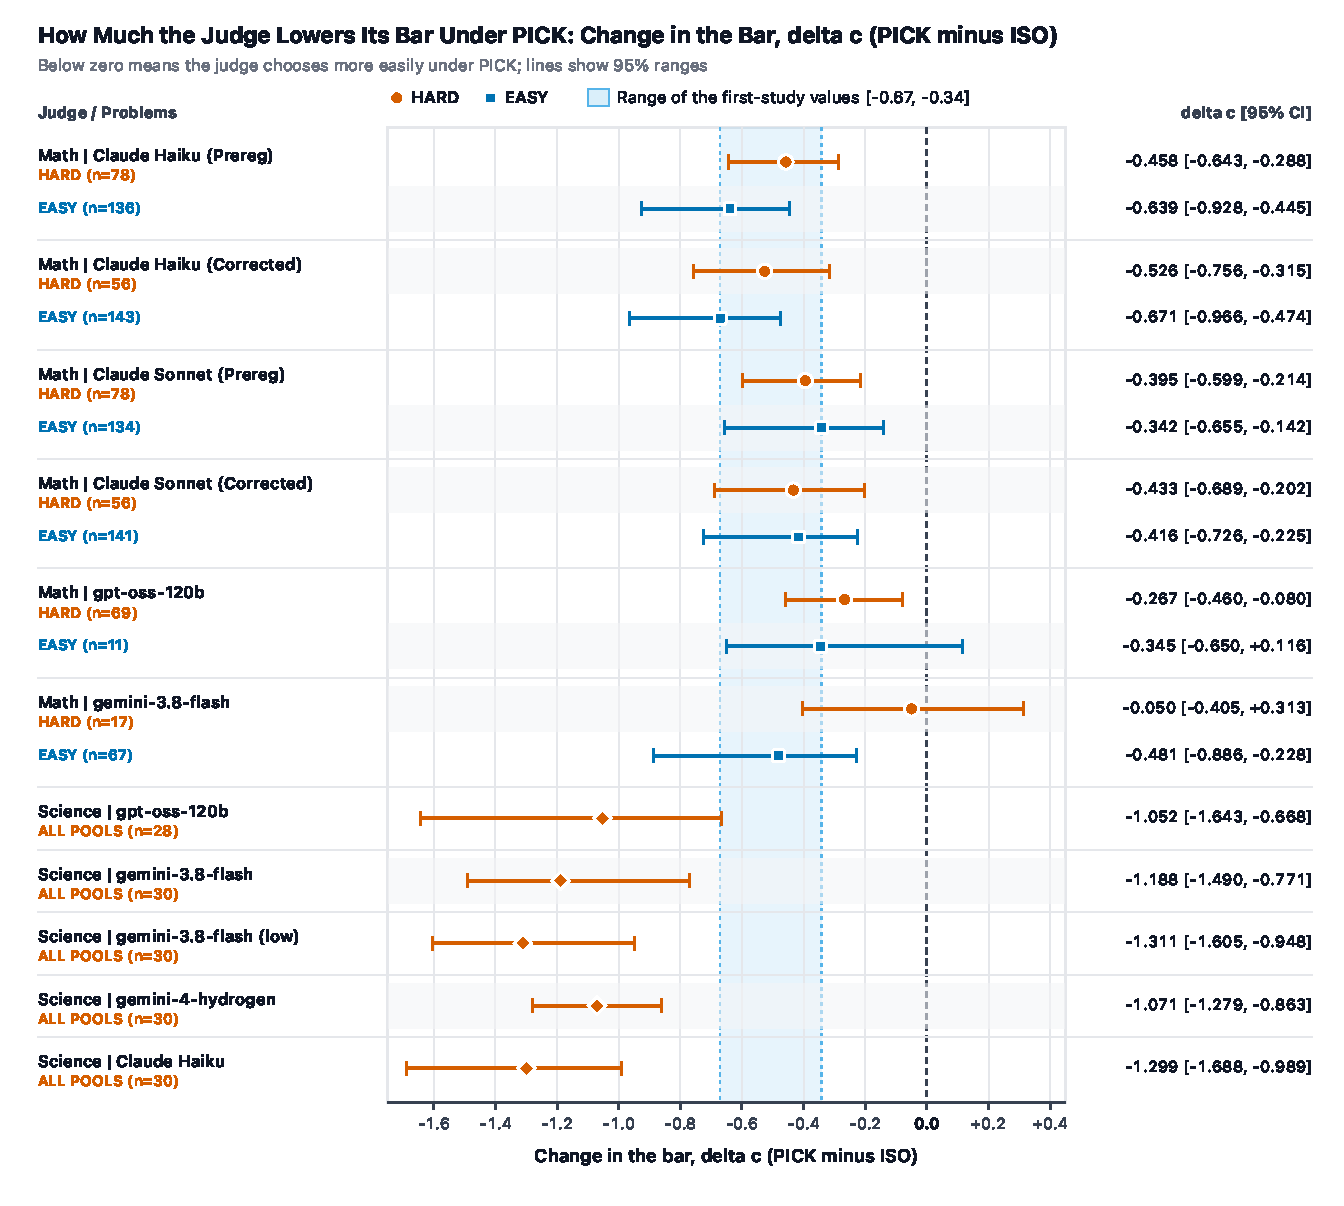
\includegraphics[width=0.92\textwidth]{figures/fig1_criterion_shift}
\caption{Paired criterion shift $\Delta c$ (\texttt{PICK} minus \texttt{ISO}) with \res{lvl95} item-bootstrap intervals across v1 MathArena strata (\texttt{claude-haiku-5-5}, \texttt{claude-sonnet-5-5}), v2 judge-family-excluded math (C6), and v2 ResearchBench hypotheses (C9). Negative $\Delta c$ means a more liberal threshold under \texttt{PICK}. The shaded band spans the eight v1 point estimates; it is a visual reference, not a prediction interval. ResearchBench rows are not stratified by solvability, and their intervals ignore clustering within 10 papers (Table~\ref{tab:science} gives paper-clustered intervals).}
\label{fig:criterion}
\end{figure*}

\begin{figure*}[t]
\centering
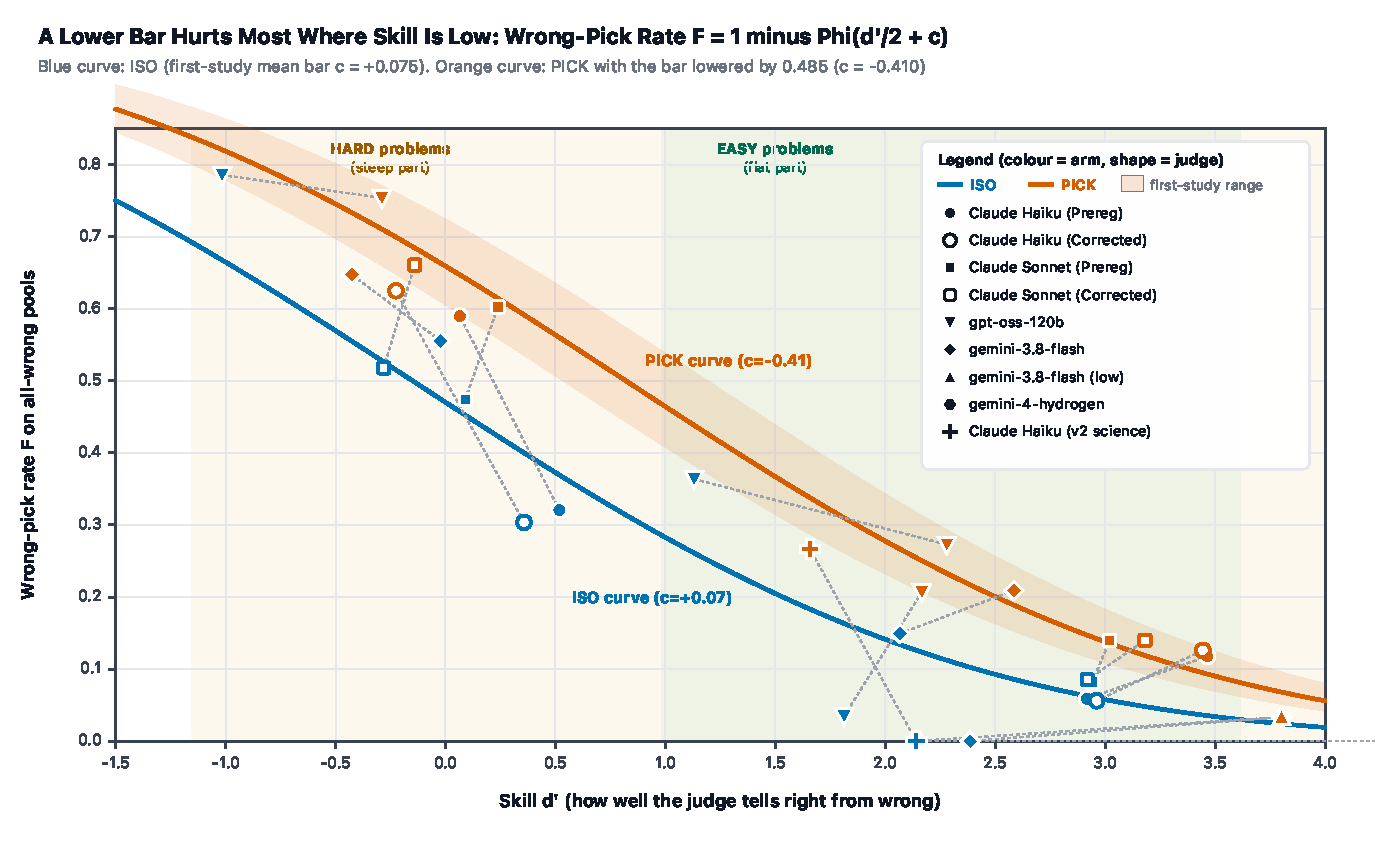
\includegraphics[width=0.92\textwidth]{figures/fig2_sdt_law_curve}
\caption{The criterion-shift account: $F = 1 - \Phi(d'/2 + c)$ for baseline \texttt{ISO} and shifted \texttt{PICK}. On high-sensitivity SOLVED pools (flat right tail), a constant $\Delta c$ produces a small raw rise in $F$. On low-sensitivity UNSOLVED pools ($d' \approx 0$, steep central slope), the identical shift produces a large rise. Curves use the mean \texttt{ISO} criterion and mean $\Delta c$ of the eight v1 cells, and the shaded band spans the range of the v1 $\Delta c$ estimates; dotted connectors join the \texttt{ISO} and \texttt{PICK} points of one judge and stratum. Several v2 points sit far from both curves, which is the visual form of the mixed C6 and C9 results.}
\label{fig:sdtlaw}
\end{figure*}

\paragraph{Exploratory v1 anchor.}
Table~\ref{tab:v1sdt} summarizes the v1 C3 aligned SDT results across \texttt{claude-haiku-5-5} and \texttt{claude-sonnet-5-5}. Across all eight judge-by-stratum cells (pre-registered and audited/corrected), $\Delta c$ lies strictly below zero (between \res{c3sp_s_pi_dc} and \res{c3hc_s_pi_dc}). Sensitivity loss ($\Delta d' < 0$) is specific to \texttt{claude-haiku-5-5} UNSOLVED (corrected \res{c3hc_u_pi_ddp}, \res{c3hc_u_pi_ddp_ci}), whereas \texttt{claude-sonnet-5-5} UNSOLVED (\res{c3sc_u_pi_ddp}, \res{c3sc_u_pi_ddp_ci}) and both SOLVED strata show CIs spanning zero. On this account the apparent ``unsolved specificity'' of raw false-choice gaps arises from where each stratum sits on the Gaussian tail, not because SOLVED items escape the criterion shift. Because this account was formulated after inspecting v1 C3 outcomes, v1 provides exploratory motivation and v2 provides confirmatory tests.

\begin{table*}[t]
\centering\footnotesize
\setlength{\tabcolsep}{4.5pt}
\begin{tabular}{llrrrrr}
\toprule
Judge & Stratum (cohort) & $N$ & $F_{\mathrm{ISO}}$ & $F_{\mathrm{PICK}}$ & $\Delta d'$ [\res{lvl95} CI] & $\Delta c$ [\res{lvl95} CI] \\
\midrule
\texttt{claude-haiku-5-5} & UNSOLVED (prereg) & \res{c3hp_u_pi_n} & \res{c3hp_u_iso_f} & \res{c3hp_u_pick_f} & \res{c3hp_u_pi_ddp} \res{c3hp_u_pi_ddp_ci} & \res{c3hp_u_pi_dc} \res{c3hp_u_pi_dc_ci} \\
\texttt{claude-haiku-5-5} & SOLVED (prereg) & \res{c3hp_s_pi_n} & \res{c3hp_s_iso_f} & \res{c3hp_s_pick_f} & \res{c3hp_s_pi_ddp} \res{c3hp_s_pi_ddp_ci} & \res{c3hp_s_pi_dc} \res{c3hp_s_pi_dc_ci} \\
\texttt{claude-haiku-5-5} & UNSOLVED (corrected) & \res{c3hc_u_pi_n} & \res{c3hc_u_iso_f} & \res{c3hc_u_pick_f} & \res{c3hc_u_pi_ddp} \res{c3hc_u_pi_ddp_ci} & \res{c3hc_u_pi_dc} \res{c3hc_u_pi_dc_ci} \\
\texttt{claude-haiku-5-5} & SOLVED (corrected) & \res{c3hc_s_pi_n} & \res{c3hc_s_iso_f} & \res{c3hc_s_pick_f} & \res{c3hc_s_pi_ddp} \res{c3hc_s_pi_ddp_ci} & \res{c3hc_s_pi_dc} \res{c3hc_s_pi_dc_ci} \\
\midrule
\texttt{claude-sonnet-5-5} & UNSOLVED (prereg) & \res{c3sp_u_pi_n} & \res{c3sp_u_iso_f} & \res{c3sp_u_pick_f} & \res{c3sp_u_pi_ddp} \res{c3sp_u_pi_ddp_ci} & \res{c3sp_u_pi_dc} \res{c3sp_u_pi_dc_ci} \\
\texttt{claude-sonnet-5-5} & SOLVED (prereg) & \res{c3sp_s_pi_n} & \res{c3sp_s_iso_f} & \res{c3sp_s_pick_f} & \res{c3sp_s_pi_ddp} \res{c3sp_s_pi_ddp_ci} & \res{c3sp_s_pi_dc} \res{c3sp_s_pi_dc_ci} \\
\texttt{claude-sonnet-5-5} & UNSOLVED (corrected) & \res{c3sc_u_pi_n} & \res{c3sc_u_iso_f} & \res{c3sc_u_pick_f} & \res{c3sc_u_pi_ddp} \res{c3sc_u_pi_ddp_ci} & \res{c3sc_u_pi_dc} \res{c3sc_u_pi_dc_ci} \\
\texttt{claude-sonnet-5-5} & SOLVED (corrected) & \res{c3sc_s_pi_n} & \res{c3sc_s_iso_f} & \res{c3sc_s_pick_f} & \res{c3sc_s_pi_ddp} \res{c3sc_s_pi_ddp_ci} & \res{c3sc_s_pi_dc} \res{c3sc_s_pi_dc_ci} \\
\bottomrule
\end{tabular}
\caption{Exploratory v1 C3 aligned SDT anchor (5,000 problem bootstraps, Hautus 1995 log-linear correction). Paired $\Delta c = c_{\mathrm{PICK}} - c_{\mathrm{ISO}}$ is strictly negative across all eight judge-by-stratum cells.}
\label{tab:v1sdt}
\end{table*}

\section{v2 Experimental Design}
\label{sec:design}
The v2 banks, the parser, two plan documents (\texttt{PREREGISTRATION\_V2.md}, \texttt{PREREG\_C7.md}) and the C7 job files were hashed with SHA-256 in \texttt{LOCKED.sha256} before the corresponding subject calls. This is a local lock, not a deposit with an external registry, so ``preregistered'' below means ``fixed in a hashed local file before the calls''. All subject calls went through subscription command-line clients (the Claude CLI for \texttt{claude-haiku-5-5}; the Antigravity CLI for the other judges), each from an empty working directory with an instruction not to use tools. The Antigravity client does not let us switch tools off or remove its own scaffolding, so for those judges isolation rests on the instruction. Statistics were computed by two analysis scripts (\texttt{analysis\_a.py}, \texttt{analysis\_b.py}) and compared leaf by leaf; both were written by AI agents in the same project, so this guards against coding slips more than against shared assumptions. Confidence intervals use 5,000 item-level bootstrap resamples, and $p$ values are one-sided bootstrap or exact McNemar values without multiplicity adjustment.

\begin{itemize}\setlength{\itemsep}{2pt}
\item \textbf{C4 (3x compute-matched control):} On corrected \texttt{claude-haiku-5-5} UNSOLVED pools ($N=\res{c4_n_ta}$ TA, $N=\res{c4_n_tp}$ paired TP; \res{c4_calls_ok}/\res{c4_calls_exp} calls, \res{c4_parse_pct} parsed), we run three independent \texttt{PICK} calls per pool and score majority-of-3 (\texttt{PICK\_MAJ3}, abstaining on 3-way splits) and any-of-3 (\texttt{PICK\_ANY3}) against 3-call \texttt{ISO}.
\item \textbf{C5 (own-answer removal and chosen-candidate removal):} On the $N=\res{c5o_all_n}$ v1 UNSOLVED TA pools containing exactly one answer matching Haiku's own SOLVE attempt ($N=\res{c5o_corr_n}$ after the v1 label and stratum audit), we remove that candidate without replacement and run \texttt{PICK-2}, compared with the stored v1 \texttt{ISO} verdicts on the two retained candidates (\texttt{ISO-2}). Second, following the removal-without-replacement procedure of \citet{wells1993what}, which tests the relative-judgment account of \citet{wells1984psychology}, on $N=\res{c5w_n}$ TA pools where Haiku chose a wrong candidate in v1 \texttt{PICK} we remove the chosen candidate and run \texttt{PICK-2} on the remaining two.
\item \textbf{C6 (judge-family-excluded math):} $N=\res{c6_n_problems}$ MathArena and arXivMath problems (50 contest, 50 arXivMath), with no GPT and no Gemini candidates in any pool and rotated TP target positions, judged by \texttt{gpt-oss-120b-medium} and \texttt{gemini-3.8-flash-medium}. Each judge first makes two \texttt{SOLVE} attempts, which define its own \texttt{SOLVED\_M} (both right), \texttt{UNSOLVED\_M} (both wrong) and \texttt{MIXED\_M} strata.
\item \textbf{C9 and C8 (ResearchBench hypotheses and low thinking):} From 10 ResearchBench papers \citep{liu2025researchbench} we build $N=\res{c9_n_items}$ TA and $N=\res{c9_n_items}$ TP four-candidate hypothesis pools: three draws of wrong hypotheses per paper, with the paper's one ground-truth hypothesis reused across its three TP pools and verified in isolation once per judge. Judges: \texttt{gpt-oss-120b-medium}, \texttt{gemini-3.8-flash-medium}, \texttt{gemini-3.8-flash-low} (C8, reduced thinking), \texttt{gemini-4-hydrogen-medium} and \texttt{claude-haiku-5-5}.
\item \textbf{C7 (mitigations):} Fixed in \texttt{PREREG\_C7.md}, against \texttt{PICK} (M0) and \texttt{ISO}: \textbf{M1} (\texttt{ISO}-filter-then-\texttt{PICK}: $k=0$ accepted candidates gives \texttt{NONE}, $k=1$ gives that candidate, $k \ge 2$ triggers one \texttt{PICK}-$k$ tie-break call), \textbf{M2} (one pooled call that must look for a concrete error in each candidate, with a fixed confidence threshold $\tau = 4$ on a 1 to 5 scale) and \textbf{M3} (a known wrong solution from another problem inserted into each 3-candidate pool, position balanced). The Haiku math leg uses a seeded random subset of 40 of the 56 paired C4 problems.
\end{itemize}

\paragraph{Deviations from the locked plans.}
(i) C4 was planned on the v1 preregistered stratum (90 TA, 78 TP) with the corrected stratum as sensitivity; only the corrected stratum was run. (ii) The C5 fresh-\texttt{ISO} drift check and the 45 pool sensitivity set were not run. (iii) The C6 plan named other judge models and the v1 pool bank; we ran the two judges available on our subscription route on a new family-excluded bank, locked before its calls, and did not run the planned regression on solvability. (iv) The C6 gate required at least 25 problems in each of \texttt{SOLVED\_M} and \texttt{UNSOLVED\_M}; neither judge meets it (Section~\ref{sec:c6}), so by our own rule the per-stratum C6 results are descriptive. (v) C9 pools have four candidates, not three, and come from 10 papers. Our \texttt{ISO} gate required a nonzero acceptance rate for wrong candidates; only \texttt{gpt-oss-120b-medium} meets it on C9, because the other four configurations accepted no wrong hypothesis in isolation. (vi) C7 follows the later \texttt{PREREG\_C7.md}: a 40 problem subset instead of the full stratum, M3 added, and no check on SOLVED pools. (vii) After the lock we found two mechanical parser gaps (algebraically equivalent \texttt{SOLVE} answers graded as wrong in 14 files, and bold or bare boxed final lines in 10 \texttt{gpt-oss-120b-medium} files). The locked parser is unchanged; an extension handles these cases and both analysis scripts apply the same rules. The fix moves some C6 problems from \texttt{UNSOLVED\_M} to \texttt{SOLVED\_M}. (viii) The planned blind human audit of the v1 labels has not been done.

\section{Results}

\subsection{Compute Matching Does Not Eliminate the Penalty (C4)}
Across \res{c4_tok_n} paired TA+TP pools, 3x repeat-\texttt{PICK} matches 3-call \texttt{ISO} in output+thinking token budget: median tokens are \res{c4_tok_pick} vs \res{c4_tok_iso}, a median ratio of \res{c4_tok_ratio}, inside our planned $[0.90, 1.10]$ band. By pool type the ratio is \res{c4_tok_ratio_ta} on TA pools and \res{x_c4_tok_ratio_tp} on TP pools, so on TP pools repeat-\texttt{PICK} used somewhat fewer tokens than \texttt{ISO} and falls just outside the band.

With compute matched this closely, the false-choice excess does not shrink. On corrected UNSOLVED TA pools ($N=\res{c4_n_ta}$), \texttt{PICK\_MAJ3} chooses a wrong candidate in \res{c4_ta_maj3} (\res{c4_ta_maj3_ci}) of pools, matching single-call \texttt{PICK\_1X} (\res{c4_ta_pick1x}, contrast \res{c4_d_maj3_p1x}, \res{c4_d_maj3_p1x_ci}) and exceeding \texttt{ISO\_any} (\res{c4_ta_iso}) by \res{c4_d_maj3_iso} (\res{c4_d_maj3_iso_ci}, one-sided $p$ \res{c4_d_maj3_iso_p}). Union aggregation (\texttt{PICK\_ANY3}) worsens TA false choices to \res{c4_ta_any3} (contrast vs \texttt{ISO\_any}: \res{c4_d_any3_iso}, \res{c4_d_any3_iso_ci}). On aligned TA+TP SDT ($N=\res{c4_n_tp}$), \texttt{PICK\_MAJ3} shifts criterion by \res{c4_sdtd_maj3_iso_dc} (\res{c4_sdtd_maj3_iso_dc_ci}) and lowers sensitivity by \res{c4_sdtd_maj3_iso_ddp} (\res{c4_sdtd_maj3_iso_ddp_ci}) relative to \texttt{ISO}. For this judge and stratum, the pooled false-choice excess is therefore not an artifact of 1x vs 3x test-time compute.

\subsection{Own-Answer Removal and Wells Removal (C5)}
In v1 C3, 46 of 90 UNSOLVED TA pools contained an answer matching Haiku's own wrong SOLVE reply. Removing that own-answer candidate without replacement (C5, \res{c5o_ok}/\res{c5o_exp} calls, \res{c5o_parse_pct} parsed) leaves a gap between \texttt{PICK-2} and \texttt{ISO-2}: across all \res{c5o_all_n} single-own-answer pools, \texttt{PICK-2} chooses a wrong candidate in \res{c5o_all_pick2} (\res{c5o_all_pick2_ci}) vs \res{c5o_all_iso2} (\res{c5o_all_iso2_ci}) for \texttt{ISO-2}, giving $d_{\mathrm{C5}} = \res{c5o_all_dc5}$ (\res{c5o_all_dc5_ci}, one-sided $p$ \res{c5o_all_dc5_p}). On the audited subset ($N=\res{c5o_corr_n}$), $d_{\mathrm{C5}} = \res{c5o_corr_dc5}$ (\res{c5o_corr_dc5_ci}, $p$ \res{c5o_corr_dc5_p}). Because C5 inherits v1 pools, we separate remaining 2-candidate pools with zero Claude candidates ($N=\res{c5o_all_cl0_n}$: \texttt{PICK-2} \res{c5o_all_cl0_pick2} vs \texttt{ISO-2} \res{c5o_all_cl0_iso2}, $d_{\mathrm{C5}} = \res{c5o_all_cl0_dc5}$, \res{c5o_all_cl0_dc5_ci}) from pools retaining at least one Claude candidate ($N=\res{c5o_all_cl1_n}$: \texttt{PICK-2} \res{c5o_all_cl1_pick2} vs \texttt{ISO-2} \res{c5o_all_cl1_iso2}, $d_{\mathrm{C5}} = \res{c5o_all_cl1_dc5}$, \res{c5o_all_cl1_dc5_ci}). Own-answer self-recognition is therefore not the sole driver of the lineup effect, though the zero-Claude C5 subgroup is small.

In the Wells removal-without-replacement test ($N=\res{c5w_n}$, \res{c5w_parse_pct} parsed), after deleting the wrong candidate Haiku originally picked in C3, Haiku still picked one of the two remaining wrong candidates in \res{c5w_pick2} (\res{c5w_pick2_ci}) of pools, exceeding both the proportional $2/3$ baseline (\res{c5w_prop_base}, difference \res{c5w_vs_prop}) and \texttt{ISO-2} (\res{c5w_iso2}, paired difference \res{c5w_diff}, \res{c5w_diff_ci}, $p$ \res{c5w_diff_p}). The pattern resembles the eyewitness finding that removing the chosen lineup member moves many choices to another member instead of to ``not present.'' The proportional baseline is descriptive and has no interval.

\subsection{Scientific Hypotheses (C9) and Thinking Budget (C8)}
Table~\ref{tab:science} and Figure~\ref{fig:crossvendor}(b) report the five judge configurations on the \res{c9_n_items} TA and \res{c9_n_items} TP ResearchBench pools (1,250 calls; parse rates \res{c9_haiku_parse_pct}, \res{c9_gptoss_parse_pct}, \res{c9_gemini_parse_pct}, \res{c9_gemlow_parse_pct} and \res{c9_hydro_parse_pct} in table order). The estimated criterion shift $\Delta c$ is negative for every configuration, also when the bootstrap resamples the 10 papers instead of the 30 pools. The reasons differ by judge, and the sample is small.

\begin{table*}[t]
\centering\footnotesize
\setlength{\tabcolsep}{4pt}
\begin{tabular}{lrrrrrrr}
\toprule
Judge (ResearchBench, $N=\res{c9_n_items}$) & TA \texttt{ISO} & TA \texttt{EACH} & TA \texttt{PICK} & TP \texttt{ISO} & TP \texttt{PICK} & $\Delta c$ [item CI] & [paper CI] \\
\midrule
\texttt{claude-haiku-5-5} & \res{c9_haiku_ta_iso} & \res{c9_haiku_ta_each} & \res{c9_haiku_ta_pick} & \res{c9_haiku_tp_iso} & \res{c9_haiku_tp_pick} & \res{c9_haiku_pi_dc} \res{c9_haiku_pi_dc_ci} & \res{x_c9_haiku_dc_ci} \\
\texttt{gpt-oss-120b-medium} & \res{c9_gptoss_ta_iso} & \res{c9_gptoss_ta_each} & \res{c9_gptoss_ta_pick} & \res{c9_gptoss_tp_iso} & \res{c9_gptoss_tp_pick} & \res{c9_gptoss_pi_dc} \res{c9_gptoss_pi_dc_ci} & \res{x_c9_gptoss_dc_ci} \\
\texttt{gemini-3.8-flash-medium} & \res{c9_gemini_ta_iso} & \res{c9_gemini_ta_each} & \res{c9_gemini_ta_pick} & \res{c9_gemini_tp_iso} & \res{c9_gemini_tp_pick} & \res{c9_gemini_pi_dc} \res{c9_gemini_pi_dc_ci} & \res{x_c9_gemini_dc_ci} \\
\texttt{gemini-3.8-flash-low} (C8) & \res{c9_gemlow_ta_iso} & \res{c9_gemlow_ta_each} & \res{c9_gemlow_ta_pick} & \res{c9_gemlow_tp_iso} & \res{c9_gemlow_tp_pick} & \res{c9_gemlow_pi_dc} \res{c9_gemlow_pi_dc_ci} & \res{x_c9_gemlow_dc_ci} \\
\texttt{gemini-4-hydrogen-medium} & \res{c9_hydro_ta_iso} & \res{c9_hydro_ta_each} & \res{c9_hydro_ta_pick} & \res{c9_hydro_tp_iso} & \res{c9_hydro_tp_pick} & \res{c9_hydro_pi_dc} \res{c9_hydro_pi_dc_ci} & \res{x_c9_hydro_dc_ci} \\
\bottomrule
\end{tabular}
\caption{C9 ResearchBench hypothesis lineups ($N=\res{c9_n_items}$ TA and \res{c9_n_items} TP pools from 10 papers, 4 candidates per pool). Both intervals are \res{lvl95} bootstrap intervals for $\Delta c$ (\texttt{PICK} minus \texttt{ISO}); the last column resamples papers and is a post hoc addition. For the Gemini rows $\Delta c$ comes almost entirely from TP pools.}
\label{tab:science}
\end{table*}

For \texttt{claude-haiku-5-5} and \texttt{gpt-oss-120b-medium}, \texttt{PICK} raises TA false choices over \texttt{ISO}: \res{c9_haiku_iso_ta_k}/\res{c9_haiku_iso_ta_n} to \res{c9_haiku_pick_ta_k}/\res{c9_haiku_pick_ta_n} for Haiku (exact McNemar $p$ \res{c9_haiku_mcn_ta_p}; the false choices fall in \res{x_c9_haiku_pfa_pick} of the 10 papers) and \res{c9_gptoss_iso_ta_k}/\res{c9_gptoss_iso_ta_n} to \res{c9_gptoss_pick_ta_k}/\res{c9_gptoss_pick_ta_n} for \texttt{gpt-oss-120b-medium} ($p$ \res{c9_gptoss_mcn_ta_p}, not significant at 0.05; \res{x_c9_gptoss_pfa_pick} papers). The three Gemini configurations stay at the TA floor under both procedures (\res{c9_gemini_iso_ta_k}/\res{c9_gemini_iso_ta_n} to \res{c9_gemini_pick_ta_k}/\res{c9_gemini_pick_ta_n}, \res{c9_gemlow_iso_ta_k}/\res{c9_gemlow_iso_ta_n} to \res{c9_gemlow_pick_ta_k}/\res{c9_gemlow_pick_ta_n}, and \res{c9_hydro_iso_ta_k}/\res{c9_hydro_iso_ta_n} to \res{c9_hydro_pick_ta_k}/\res{c9_hydro_pick_ta_n}).

On TP pools every judge selects the right hypothesis far more often under \texttt{PICK}. In isolation the judges accepted the ground-truth hypothesis for only \res{x_c9_haiku_gold}, \res{x_c9_gptoss_gold}, \res{x_c9_gemini_gold}, \res{x_c9_gemlow_gold} and \res{x_c9_hydro_gold} of the 10 papers (table order), while \texttt{PICK} selected it in \res{c9_haiku_pick_tp_k}, \res{c9_gptoss_pick_tp_k}, \res{c9_gemini_pick_tp_k}, \res{c9_gemlow_pick_tp_k} and \res{c9_hydro_pick_tp_k} of \res{c9_gemini_pick_tp_n} TP pools. Because each ground-truth hypothesis was verified once and reused in three pools, the \texttt{ISO} TP rate rests on 10 verdicts per judge, and item-level tests on TP would overstate the evidence; we do not report them. For the Gemini configurations the negative $\Delta c$ therefore reflects more correct selections at almost no cost in false choices, amplified by the log-linear correction at floor and ceiling. On these pools \texttt{PICK} was simply the better procedure for those judges. This fits the account (a liberal shift is cheap when sensitivity is high), but it also shows that isolated verification has a real cost in missed correct candidates. Lowering thinking effort on \texttt{gemini-3.8-flash} (C8) changes the isolated acceptance of the ground truth by one paper and leaves \texttt{PICK} unchanged.

\begin{figure*}[t]
\centering
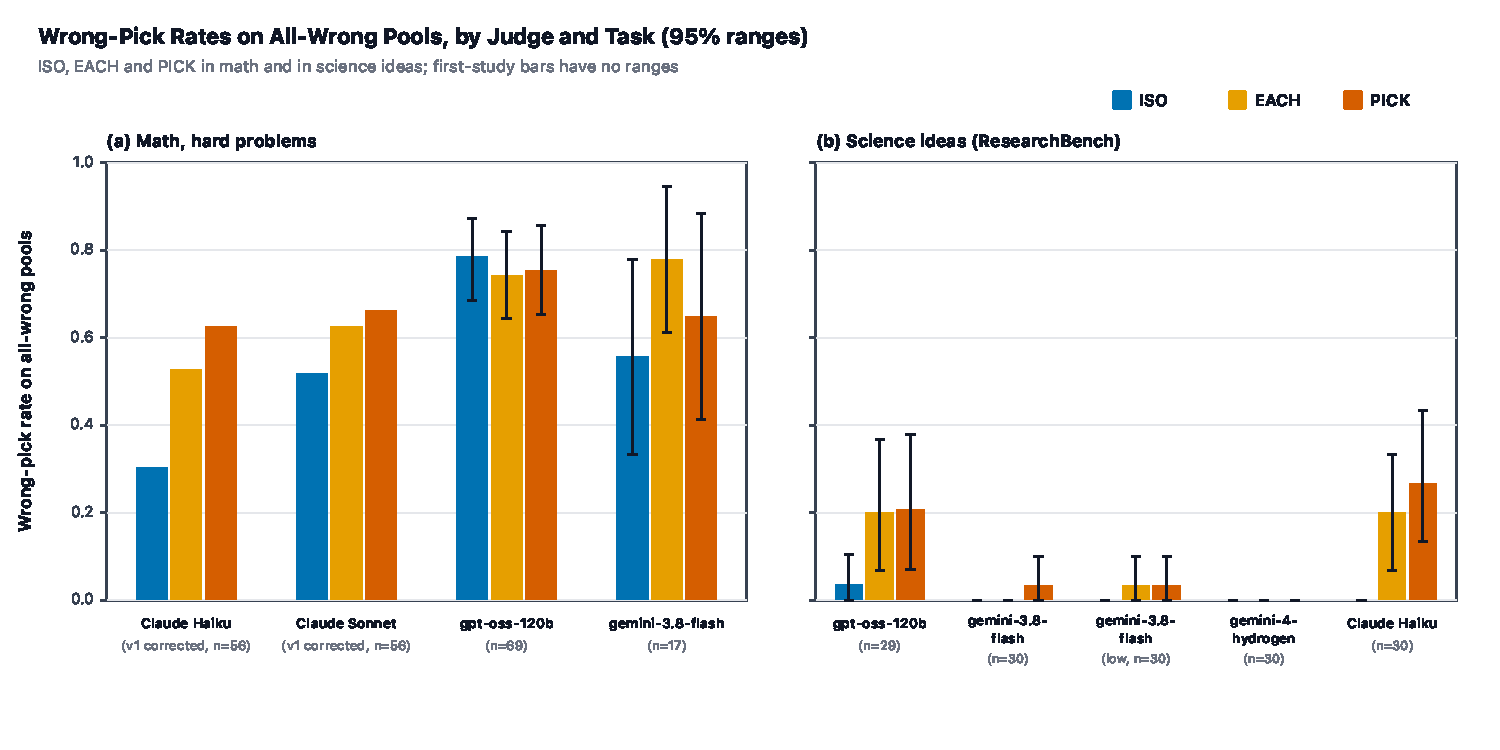
\includegraphics[width=0.95\textwidth]{figures/fig3_crossvendor_domains}
\caption{TA false-choice rates under \texttt{ISO}, \texttt{EACH} and \texttt{PICK} with \res{lvl95} item-bootstrap intervals. (a) Mathematics, UNSOLVED stratum of each judge: the Claude bars are v1 pools (not family-excluded, shown without intervals), the other two are the family-excluded C6 pools. (b) ResearchBench hypothesis lineups, five judge configurations.}
\label{fig:crossvendor}
\end{figure*}

\subsection{Judge-Family-Excluded Math (C6)}
\label{sec:c6}
Table~\ref{tab:c6math} reports the family-excluded MathArena and arXivMath replication (1,000 calls per judge; \res{c6_gptoss_parse_pct} parsed for \texttt{gpt-oss-120b-medium} and \res{c6_gemini_parse_pct} for \texttt{gemini-3.8-flash-medium}; no own-family candidate in any pool). The strata are unbalanced in opposite directions: \texttt{gpt-oss-120b-medium} has $N_{\mathrm{UNSOLVED}}=\res{c6_gptoss_n_u}$ (\res{c6_gptoss_n_u_contest} contest, \res{c6_gptoss_n_u_arxiv} arXivMath) and $N_{\mathrm{SOLVED}}=\res{c6_gptoss_n_s}$, while \texttt{gemini-3.8-flash-medium} has $N_{\mathrm{UNSOLVED}}=\res{c6_gemini_n_u}$ (\res{c6_gemini_n_u_contest} contest, \res{c6_gemini_n_u_arxiv} arXivMath) and $N_{\mathrm{SOLVED}}=\res{c6_gemini_n_s}$. Neither judge has 25 problems in both strata, so both miss our stratum-size gate and the per-stratum rows are descriptive. The $N$ column of Table~\ref{tab:c6math} counts the problems that enter the paired \texttt{PICK} minus \texttt{ISO} contrast, which is one fewer than the stratum size in three rows and 98 of 100 overall.

\paragraph{The planned primary test is not supported.} The plan's primary C6 test was a higher TA false-choice rate under \texttt{PICK} than under \texttt{ISO} on \texttt{UNSOLVED\_M}. For \texttt{gpt-oss-120b-medium} the difference is \res{c6_gptoss_u_pi_df} (\res{c6_gptoss_u_pi_df_ci}), with \texttt{ISO} at \res{c6_gptoss_u_ta_iso} and \texttt{PICK} at \res{c6_gptoss_u_ta_pick}; over all problems it is \res{c6_gptoss_all_pi_df} (\res{c6_gptoss_all_pi_df_ci}). For \texttt{gemini-3.8-flash-medium} it is \res{c6_gemini_u_pi_df} (\res{c6_gemini_u_pi_df_ci}) on \texttt{UNSOLVED\_M} and \res{c6_gemini_all_pi_df} (\res{c6_gemini_all_pi_df_ci}) over all problems. On \texttt{UNSOLVED\_M}, where the test was planned, neither interval excludes zero. Only the all-problem difference for \texttt{gemini-3.8-flash-medium} is borderline (lower bound at zero), and for \texttt{gpt-oss-120b-medium} the sign is reversed. The raw false-choice excess seen for Claude judges in v1 is at most weakly present here.

\paragraph{The criterion shift is negative overall.} Over all problems $\Delta c$ is \res{c6_gptoss_all_pi_dc} (\res{c6_gptoss_all_pi_dc_ci}) for \texttt{gpt-oss-120b-medium} and \res{c6_gemini_all_pi_dc} (\res{c6_gemini_all_pi_dc_ci}) for \texttt{gemini-3.8-flash-medium}. In both cases the shift shows up mostly as more correct selections on TP pools (\res{c6_gptoss_all_tp_iso} to \res{c6_gptoss_all_tp_pick}, and \res{c6_gemini_all_tp_iso} to \res{c6_gemini_all_tp_pick}). By stratum the picture is uneven: for \texttt{gpt-oss-120b-medium}, $\Delta c$ is \res{c6_gptoss_u_pi_dc} (\res{c6_gptoss_u_pi_dc_ci}) on \texttt{UNSOLVED\_M} and \res{c6_gptoss_s_pi_dc} (\res{c6_gptoss_s_pi_dc_ci}, $N=\res{c6_gptoss_s_pi_n}$) on \texttt{SOLVED\_M}; for \texttt{gemini-3.8-flash-medium} it is \res{c6_gemini_s_pi_dc} (\res{c6_gemini_s_pi_dc_ci}) on \texttt{SOLVED\_M} and \res{c6_gemini_u_pi_dc} (\res{c6_gemini_u_pi_dc_ci}, $N=\res{c6_gemini_u_pi_n}$) on \texttt{UNSOLVED\_M}, where the interval is wide and centered near zero. \texttt{gpt-oss-120b-medium} is a credulous isolated verifier (it accepts \res{c6_gptoss_cal_w} of wrong candidates one at a time, against \res{c6_gemini_cal_w} for \texttt{gemini-3.8-flash-medium}), so its 3-call \texttt{ISO} already accepts some wrong candidate in most all-wrong pools and has little room to look better than \texttt{PICK}.

\paragraph{Out-of-sample prediction.} Our plan included a quantitative test: take $\Delta c$ from a judge's SOLVED stratum, add it to that judge's \texttt{ISO} criterion on UNSOLVED, and predict the UNSOLVED \texttt{PICK} false-choice rate from $F = 1 - \Phi(d'/2 + c)$. For \texttt{gpt-oss-120b-medium} the prediction is \res{x_h3_gptoss_pred} against an observed \res{c6_gptoss_u_pick_f} (\res{c6_gptoss_u_pick_f_ci}), outside the interval. For \texttt{gemini-3.8-flash-medium} it is \res{x_h3_gemini_pred} against \res{c6_gemini_u_pick_f} (\res{c6_gemini_u_pick_f_ci}), inside an interval too wide to be informative at $N=\res{c6_gemini_u_pi_n}$. Both use a SOLVED or UNSOLVED stratum below the gate. We read this as no support yet for a constant shift across strata outside the Claude judges. We computed this check at finalisation with a separate script.

\begin{table*}[t]
\centering\footnotesize
\setlength{\tabcolsep}{4.5pt}
\begin{tabular}{llrrrrrr}
\toprule
Judge (C6 math, family-excluded) & Stratum & $N$ & TA \texttt{ISO} & TA \texttt{PICK} & TP \texttt{ISO} & TP \texttt{PICK} & $\Delta c$ [\res{lvl95} CI] \\
\midrule
\texttt{gpt-oss-120b-medium} & ALL & \res{c6_gptoss_all_pi_n} & \res{c6_gptoss_all_ta_iso} & \res{c6_gptoss_all_ta_pick} & \res{c6_gptoss_all_tp_iso} & \res{c6_gptoss_all_tp_pick} & \res{c6_gptoss_all_pi_dc} \res{c6_gptoss_all_pi_dc_ci} \\
\texttt{gpt-oss-120b-medium} & UNSOLVED\_M & \res{c6_gptoss_u_pi_n} & \res{c6_gptoss_u_ta_iso} & \res{c6_gptoss_u_ta_pick} & \res{c6_gptoss_u_tp_iso} & \res{c6_gptoss_u_tp_pick} & \res{c6_gptoss_u_pi_dc} \res{c6_gptoss_u_pi_dc_ci} \\
\texttt{gpt-oss-120b-medium} & SOLVED\_M & \res{c6_gptoss_s_pi_n} & \res{c6_gptoss_s_ta_iso} & \res{c6_gptoss_s_ta_pick} & \res{c6_gptoss_s_tp_iso} & \res{c6_gptoss_s_tp_pick} & \res{c6_gptoss_s_pi_dc} \res{c6_gptoss_s_pi_dc_ci} \\
\midrule
\texttt{gemini-3.8-flash-medium} & ALL & \res{c6_gemini_all_pi_n} & \res{c6_gemini_all_ta_iso} & \res{c6_gemini_all_ta_pick} & \res{c6_gemini_all_tp_iso} & \res{c6_gemini_all_tp_pick} & \res{c6_gemini_all_pi_dc} \res{c6_gemini_all_pi_dc_ci} \\
\texttt{gemini-3.8-flash-medium} & UNSOLVED\_M & \res{c6_gemini_u_pi_n} & \res{c6_gemini_u_ta_iso} & \res{c6_gemini_u_ta_pick} & \res{c6_gemini_u_tp_iso} & \res{c6_gemini_u_tp_pick} & \res{c6_gemini_u_pi_dc} \res{c6_gemini_u_pi_dc_ci} \\
\texttt{gemini-3.8-flash-medium} & SOLVED\_M & \res{c6_gemini_s_pi_n} & \res{c6_gemini_s_ta_iso} & \res{c6_gemini_s_ta_pick} & \res{c6_gemini_s_tp_iso} & \res{c6_gemini_s_tp_pick} & \res{c6_gemini_s_pi_dc} \res{c6_gemini_s_pi_dc_ci} \\
\bottomrule
\end{tabular}
\caption{C6 judge-family-excluded math ($N=\res{c6_n_problems}$ problems, half contest and half arXivMath; no own-family candidate in any pool). Per-stratum rows are descriptive because both judges miss the stratum-size gate.}
\label{tab:c6math}
\end{table*}

\subsection{Mitigations (C7)}
Table~\ref{tab:mitigation} and Figure~\ref{fig:mitigation} compare the three mitigation arms on the same $N=\res{c7_m1_n}$ corrected UNSOLVED \texttt{claude-haiku-5-5} math problems, alongside M2 on C6 math and ResearchBench pools. One caution applies to every Haiku math number in this section. The 40 problems were drawn by a seeded shuffle that does not look at outcomes, but the draw happened to be favorable to \texttt{ISO}: stored \texttt{ISO} verdicts accept some wrong candidate in \res{x_c7_sub_k} of the 40 selected TA pools against \res{x_c7_rest_k} of the \res{x_c7_rest_n} left out (\res{x_c7_full_k} of \res{x_c7_full_n}, or \res{x_c7_full_f}, on the full paired stratum; a draw this low has hypergeometric probability \res{x_c7_tail}), while the \texttt{PICK} rate on the subset matches the full stratum. The gap between \texttt{PICK} and anything built on \texttt{ISO} is therefore probably overstated here; the C4 contrast on the full stratum (\res{c4_d_maj3_iso}) is the better guide to its size.

\begin{figure*}[t]
\centering
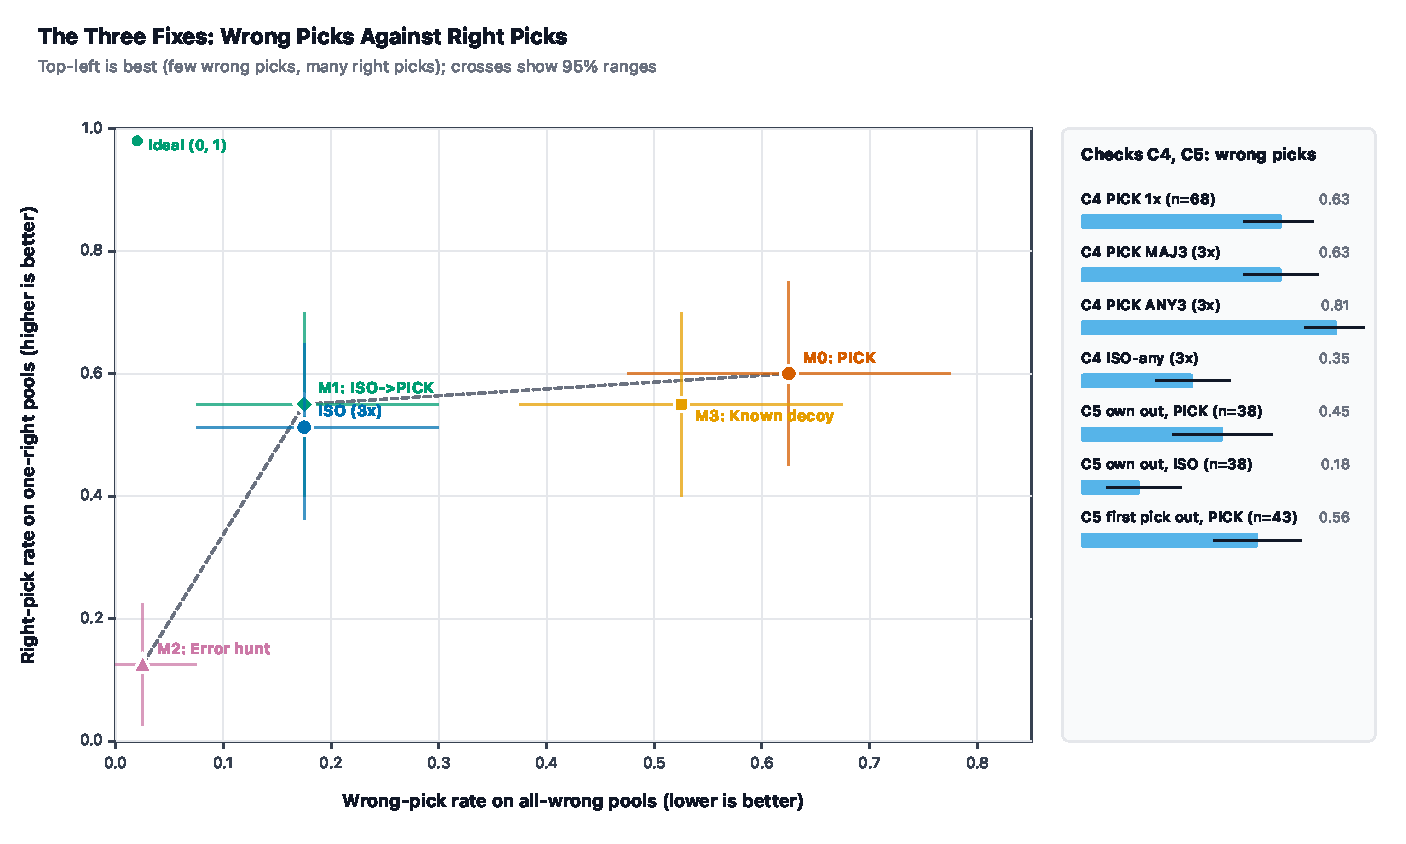
\includegraphics[width=0.94\textwidth]{figures/fig4_mitigation_frontier}
\caption{Operating points on the 40 problem UNSOLVED \texttt{claude-haiku-5-5} math subset: TA false-choice rate against TP correct selection rate, with \res{lvl95} bootstrap crosshairs. M1 and \texttt{ISO} share the same false-choice rate. Right panel: TA false-choice rates in the C4 and C5 controls.}
\label{fig:mitigation}
\end{figure*}

\begin{table*}[t]
\centering\footnotesize
\setlength{\tabcolsep}{3.5pt}
\resizebox{\textwidth}{!}{%
\begin{tabular}{llrrrrr}
\toprule
Domain / Judge & Arm & $N$ & TA $F$ & TP $H$ & $d'$ [\res{lvl95} CI] & $c$ [\res{lvl95} CI] \\
\midrule
Math UNSOLVED, \texttt{claude-haiku-5-5} & M0 (\texttt{PICK}) & \res{c7_m1_n} & \res{c7_m1_pick_f} & \res{c7_m1_pick_h} & \res{c7_m1_pick_dp} \res{c7_m1_pick_dp_ci} & \res{c7_m1_pick_c} \res{c7_m1_pick_c_ci} \\
Math UNSOLVED, \texttt{claude-haiku-5-5} & \texttt{ISO} (3x) & \res{c7_m1_n} & \res{c7_m1_iso_f} & \res{c7_m1_iso_h} & \res{c7_m1_iso_dp} \res{c7_m1_iso_dp_ci} & \res{c7_m1_iso_c} \res{c7_m1_iso_c_ci} \\
Math UNSOLVED, \texttt{claude-haiku-5-5} & \textbf{M1 (\texttt{ISO}$\to$\texttt{PICK})} & \res{c7_m1_n} & \res{c7_m1_m1_f} & \res{c7_m1_m1_h} & \res{c7_m1_m1_dp} \res{c7_m1_m1_dp_ci} & \res{c7_m1_m1_c} \res{c7_m1_m1_c_ci} \\
Math UNSOLVED, \texttt{claude-haiku-5-5} & M2 (Falsify Gate) & \res{c7_m2h_n} & \res{c7_m2h_g4_f} & \res{c7_m2h_g4_h} & \res{c7_m2h_g4_dp} \res{c7_m2h_g4_dp_ci} & \res{c7_m2h_g4_c} \res{c7_m2h_g4_c_ci} \\
Math UNSOLVED, \texttt{claude-haiku-5-5} & M3 (Known Foil) & \res{c7_m3_n} & \res{c7_m3_f} & \res{c7_m3_h} & \res{c7_m3_dp} \res{c7_m3_dp_ci} & \res{c7_m3_c} \res{c7_m3_c_ci} \\
\midrule
Math C6, \texttt{gpt-oss-120b-medium} & M2 (Falsify Gate) & \res{c7_m2m_gptoss_n} & \res{c7_m2m_gptoss_g4_f} & \res{c7_m2m_gptoss_g4_h} & \res{c7_m2m_gptoss_g4_dp} \res{c7_m2m_gptoss_g4_dp_ci} & \res{c7_m2m_gptoss_g4_c} \res{c7_m2m_gptoss_g4_c_ci} \\
Math C6, \texttt{gemini-3.8-flash-medium} & M2 (Falsify Gate) & \res{c7_m2m_gemini_n} & \res{c7_m2m_gemini_g4_f} & \res{c7_m2m_gemini_g4_h} & \res{c7_m2m_gemini_g4_dp} \res{c7_m2m_gemini_g4_dp_ci} & \res{c7_m2m_gemini_g4_c} \res{c7_m2m_gemini_g4_c_ci} \\
\midrule
Science C9, \texttt{claude-haiku-5-5} & M2 (Falsify Gate) & \res{c9_n_items} & \res{c7_m2s_haiku_g4_f} & \res{c7_m2s_haiku_g4_h} & \res{c7_m2s_haiku_g4_dp} \res{c7_m2s_haiku_g4_dp_ci} & \res{c7_m2s_haiku_g4_c} \res{c7_m2s_haiku_g4_c_ci} \\
Science C9, \texttt{gpt-oss-120b-medium} & M2 (Falsify Gate) & \res{c9_n_items} & \res{c7_m2s_gptoss_g4_f} & \res{c7_m2s_gptoss_g4_h} & \res{c7_m2s_gptoss_g4_dp} \res{c7_m2s_gptoss_g4_dp_ci} & \res{c7_m2s_gptoss_g4_c} \res{c7_m2s_gptoss_g4_c_ci} \\
Science C9, \texttt{gemini-3.8-flash-medium} & M2 (Falsify Gate) & \res{c9_n_items} & \res{c7_m2s_gemini_g4_f} & \res{c7_m2s_gemini_g4_h} & \res{c7_m2s_gemini_g4_dp} \res{c7_m2s_gemini_g4_dp_ci} & \res{c7_m2s_gemini_g4_c} \res{c7_m2s_gemini_g4_c_ci} \\
Science C9, \texttt{gemini-3.8-flash-low} & M2 (Falsify Gate) & \res{c9_n_items} & \res{c7_m2s_gemlow_g4_f} & \res{c7_m2s_gemlow_g4_h} & \res{c7_m2s_gemlow_g4_dp} \res{c7_m2s_gemlow_g4_dp_ci} & \res{c7_m2s_gemlow_g4_c} \res{c7_m2s_gemlow_g4_c_ci} \\
Science C9, \texttt{gemini-4-hydrogen-medium} & M2 (Falsify Gate) & \res{c9_n_items} & \res{c7_m2s_hydro_g4_f} & \res{c7_m2s_hydro_g4_h} & \res{c7_m2s_hydro_g4_dp} \res{c7_m2s_hydro_g4_dp_ci} & \res{c7_m2s_hydro_g4_c} \res{c7_m2s_hydro_g4_c_ci} \\
\bottomrule
\end{tabular}%
}
\caption{C7 mitigation results (TA false-choice rate $F$ and TP hit rate $H$). On the Haiku math subset, M1 and \texttt{ISO} have the same false-choice rate; M1 differs from \texttt{ISO} only in how it breaks ties among accepted candidates.}
\label{tab:mitigation}
\end{table*}

On the Haiku math subset ($N=\res{c7_m1_n}$) the three arms behave differently:
\begin{itemize}\setlength{\itemsep}{2pt}
\item \textbf{M1 (\texttt{ISO}-filter-then-\texttt{PICK}) equals \texttt{ISO} on false choices.} Stage 1 resolves 72 of 80 pools without a further call (48 with $k=0$, 24 with $k=1$), and \res{c7_m1_tb_ok} pools need a tie-break. M1 therefore costs the three \texttt{ISO} calls plus \res{c7_m1_extra_calls} calls per pool, against one call for \texttt{PICK}. Its TA false-choice rate is \res{c7_m1_m1_f}, identical to \texttt{ISO} (\res{c7_m1_iso_f}) and below \texttt{PICK} (\res{c7_m1_pick_f}; paired difference \res{c7_m1_mp_df}, \res{c7_m1_mp_df_ci}). Against \texttt{PICK} it moves the criterion by \res{c7_m1_mp_dc} (\res{c7_m1_crec} of the \texttt{PICK} minus \texttt{ISO} shift) and raises $d'$ from \res{c7_m1_pick_dp} to \res{c7_m1_m1_dp} (difference \res{c7_m1_mp_ddp}, \res{c7_m1_mp_ddp_ci}). Against \texttt{ISO} its only gain is the tie-break: TP hits \res{c7_m1_m1_h} vs \res{c7_m1_iso_h} (difference \res{c7_m1_mi_dh}, \res{c7_m1_mi_dh_ci}) and $d'$ difference \res{c7_m1_mi_ddp} (\res{c7_m1_mi_ddp_ci}), based on 8 pools. So M1 is best described as \texttt{ISO} with a sensible tie-break, and its advantage over \texttt{PICK} is the advantage of \texttt{ISO}.
\item \textbf{M2 (falsification-first gate) over-corrects on hard math.} On the Haiku math subset M2 drops TA false choices to \res{c7_m2h_g4_f} but TP hits fall to \res{c7_m2h_g4_h} (from \res{c7_m1_iso_h} under \texttt{ISO} and \res{c7_m1_pick_h} under \texttt{PICK}), with $c = \res{c7_m2h_g4_c}$. Its $d'$ (\res{c7_m2h_g4_dp}) is above \texttt{PICK} but not above \texttt{ISO}, so it buys nothing that \texttt{ISO} does not give at a far better hit rate. On ResearchBench pools it also removes Haiku's TA false choices (\res{c9_haiku_ta_pick} to \res{c7_m2s_haiku_g4_f}) at the cost of TP hits (\res{c9_haiku_tp_pick} to \res{c7_m2s_haiku_g4_h}). For \texttt{gpt-oss-120b-medium} on ResearchBench it roughly halves TA false choices (\res{c9_gptoss_ta_pick} to \res{c7_m2s_gptoss_g4_f}) with TP hits at \res{c7_m2s_gptoss_g4_h} (\res{c9_gptoss_tp_pick} under \texttt{PICK}), and the Gemini configurations were already near the floor. On the C6 math subset M2 gives \res{c7_m2m_gptoss_g4_f} false choices and \res{c7_m2m_gptoss_g4_h} hits for \texttt{gpt-oss-120b-medium} and \res{c7_m2m_gemini_g4_f} and \res{c7_m2m_gemini_g4_h} for \texttt{gemini-3.8-flash-medium}. The gate's effect depends strongly on judge and domain.
\item \textbf{M3 (known-foil lineup) does not help.} Haiku never selected the inserted decoy (\res{c7_m3_foil_all} across 80 pools), so the prompt was read. TA false choices on the three real wrong candidates stayed at \res{c7_m3_f} (difference from \texttt{PICK} \res{c7_m3_mp_df}, \res{c7_m3_mp_df_ci}, interval includes zero), with the criterion still well below \texttt{ISO} ($\Delta c$ vs \texttt{ISO} \res{c7_m3_mi_dc}). Rejecting an obvious decoy did not make the judge stricter about plausible wrong solutions.
\end{itemize}

\section{Limitations}
\begin{enumerate}\setlength{\itemsep}{2pt}
\item \textbf{Post hoc account.} The criterion-shift account was formed after seeing v1 data. In v2 its sign prediction holds in most cells, its constancy across strata is not established outside the Claude judges, and the one planned quantitative prediction is unsupported (Section~\ref{sec:c6}).
\item \textbf{One judge carries the mechanism controls.} C4, C5 and the M1 and M3 arms use only \texttt{claude-haiku-5-5}, on pools inherited from v1 in which most candidate sets include a Claude solution. The zero-Claude subgroup in C5 is small ($N=\res{c5o_all_cl0_n}$) and its interval touches zero.
\item \textbf{Small and clustered science sample.} C9 has 30 pools per type from 10 papers, with each ground-truth hypothesis verified once per judge. Item-level intervals understate uncertainty; Table~\ref{tab:science} adds paper-clustered intervals.
\item \textbf{Unbalanced C6 strata.} Neither non-Anthropic judge has enough problems in both solvability strata, and \texttt{UNSOLVED\_M} for \texttt{gemini-3.8-flash-medium} is almost entirely arXivMath.
\item \textbf{A favorable subset in C7.} The seeded 40 problem subset has an unusually low \texttt{ISO} false-acceptance rate, which inflates every Haiku math contrast against \texttt{PICK} in C7.
\item \textbf{Final-answer line shown to judges.} Each math candidate was shown with a line ``Final answer:'' taken from MathArena's parsed answer field. In some pools that field does not match the boxed answer in the solution text (evaluated floats, stray digits, parser artifacts): 68 of 543 v1 pools, 17 of 200 C6 pools, 9 of 124 C4 pools and 6 of 81 C5 pools. Labels are unaffected in our audit (no wrong-labelled candidate has a boxed answer equal to the reference), but judges saw an inconsistent line in those pools, the same in every arm. We have not rerun the analyses without them.
\item \textbf{Labels.} The v1 label corrections were adjudicated by AI agents. A blind human audit tool is prepared but the audit has not been done. A scripted 120 file audit found no parser errors on C6, C9 and C7 M2 replies after the extension described in Section~\ref{sec:design}.
\item \textbf{Client scaffolding.} Subscription clients add their own system prompts. C4 matches output and thinking tokens, not total context, and we could not run a bare API control.
\item \textbf{Scope.} Results are for the named model versions and effort settings, in November 2026, on short-answer math and abstract-level hypothesis selection.
\end{enumerate}

\section{Conclusion}
For \texttt{claude-haiku-5-5} on hard math, asking the judge to pick among candidates produces more false choices on all-wrong pools than verifying candidates one at a time, and this survives matched compute, removal of the judge's own answer and removal of its first choice. A more liberal criterion under pooling describes those data well. Beyond that judge the picture is mixed: the estimated criterion shift is negative overall for two other model families on family-excluded math and for all five configurations on scientific hypotheses, but the raw false-choice excess does not appear for \texttt{gpt-oss-120b-medium} on math, and for Gemini judges on hypotheses pooling mostly helps. Among the mitigations we tried, only verifying candidates in isolation before any pooled choice reduced false choices without a clear loss of correct ones on hard math, and it costs about three times the calls. Whether to pool or isolate therefore depends on how often a pool is likely to contain no correct candidate and on how discriminating the judge is in isolation; measuring both on target-absent pools is cheap and, in our view, worth doing before trusting a selection stage.

\section*{Data and code availability}
The v1 archive (plans, prompts, raw replies, grading code and analysis scripts) is public at \url{https://github.com/chaitshar/when-no-candidate-is-correct/tree/v1.0}. The v2 banks, plan documents, lock files, raw replies, both analysis scripts and the finalisation script (\texttt{scripts/final\_sensitivity.py}) are in the \texttt{v2/} folder of the same archive, release v2.0 (\url{https://github.com/chaitshar/when-no-candidate-is-correct/tree/v2.0/v2}). MathArena data carry a CC BY-NC-SA licence.

\section*{AI assistance}
The author set the research direction and constraints. AI coding agents (Google Antigravity and Claude Code) wrote the harness, ran the experiments and analyses, and drafted the paper under those constraints; an AI agent also audited the draft against the raw replies and the plan documents, which led to the deviations paragraph and several of the limitations above. ``Independent'' scripts or checks in this paper are separate AI-written programs, not human checks. The author is responsible for the content.

\bibliographystyle{plainnat}
\bibliography{refs}

\end{document}
